% ============================================================================
%  experimental_database.tex
%
%  A manuscript section on the experimental irradiated-microstructure database
%  for ferritic / ferritic-martensitic steels, and the temperature trends fitted
%  to it with neutron and ion irradiation treated as separate populations.
%
%  Meant to be \input{} into a manuscript.  Required packages:
%      \usepackage{graphicx}
%      \usepackage{booktabs}
%      \usepackage{amsmath,amssymb}
%  Figures are expected at  figures/experiments/*.png  (300 dpi) relative to the
%  main file.
%
%  Source data : FerriticSteels_RadiationDatabase.xlsx
%  Analysis    : FerriticSteelsMicroData.ipynb  (parsing, T-shift, fitting)
%  Figures     : make_experiment_figures.py -> figures/experiments/
%  Numbers     : figures/experiments/fit_summary.txt
% ============================================================================

\section{The experimental microstructure database and its temperature trends}
\label{sec:expdb}

\subsection{Data sources and trend analysis}
\label{sec:expdb:sources}

\subsubsection*{The database}

The comparison data are collected in a single workbook,
\texttt{FerriticSteels\_RadiationDatabase.xlsx}. Its five defect-population sheets
(\texttt{Neutron\_DislocLoops}, \texttt{Ion\_DislocLoops},
\texttt{Neutron\_Voids\_Swelling}, \texttt{Ion\_Voids\_Swelling} and
\texttt{Ion\_He\_Bubbles}) contribute $68$ measurement rows drawn from $38$
publications; a sixth sheet, \texttt{Loop\_fractions}, adds measurements of the
$\langle 100\rangle$ share of the loop population from a further thirteen sources
and is treated separately in Section~\ref{sec:expdb:fraction}. The alloys span the reduced-activation ferritic/martensitic (RAFM)
grades EUROFER97 and EUROFER-ODS, F82H, CLAM and RUSFER\hbox{-}EK\hbox{-}181; the
conventional ferritic/martensitic grades T91, T92, NF616/Gr.\,92, HT9 and HCM12A;
the oxide-dispersion-strengthened variants 14YWT, 14.5Cr-ODS,
14.5Cr-3.5Al(Zr)-ODS and the Y--Ti/Y--Al/Y--Al--Zr ODS series; and the model
alloys Fe-9Cr, Fe-9Cr-C, Fe-12Cr and pure iron. Each row carries a mean feature
diameter, a feature number density, a dose, an irradiation temperature, the
irradiation source and, for loops, the dominant Burgers vector.

Every point plotted in this section is labelled with the number of the paper it
was measured in (Table~\ref{tab:refs}), so points sharing a source share a label
across every panel. Those numbers are properties of the source, not of the row:
a paper contributing four rows carries the same number four times.

\subsubsection*{Reduction of the free-text cells}

The workbook records what the papers report, which is frequently not a single
number: cells such as \verb|~10-15|, \verb|<5 (black dots)|, \verb|High (>1.4)|,
\verb|~5x10^20| or \verb|~0.5 (small); <0.1 (large)| occur throughout. They are
reduced to numbers by fixed, declared rules (Table~\ref{tab:parse}); no cell is
edited by hand and no value is invented. Cells with no numeric content at all
(\texttt{N/R}, \texttt{Reported}, \texttt{Wide scatter}, \texttt{High},
\texttt{Higher than CLAM}) contribute no value for that quantity and the row is
dropped from that panel only. This is why the four panels of a given irradiation
type do not all have the same $n$: a paper may report a size but only a
qualitative density.

A row is assigned to the neutron or ion population by the irradiation source it
reports, not by the sheet it is stored in. One entry in the neutron cavity sheet
(source 17, EUROFER97 at $26$~dpa) is in fact a dual-beam Fe$^{3+}$ experiment
included there for comparison, and is treated throughout as an ion irradiation.

\begin{table}[htbp]
\centering
\caption{Rules by which a free-text database cell is reduced to a number.
Ranges are reduced geometrically for doses and number densities, which are
log-distributed, and arithmetically for sizes and temperatures.}
\label{tab:parse}
\begin{tabular}{ll}
\toprule
Cell pattern & Rule \\
\midrule
$a$--$b$ (range)               & arithmetic mean for sizes and temperatures, \\
                               & geometric mean for doses and number densities \\
\verb|~x|, $\approx x$         & value taken as $x$ \\
$<x$, $>x$                     & value taken as $x$; the row is flagged \texttt{bound} \\
\verb|(x10^22 est.)|           & recognised as a unit annotation and stripped \\
$A\times10^{k}$, $10^{k}$      & absolute scientific notation; overrides the column unit \\
$p$; $q$ (bimodal)             & the two populations are summed to a total density \\
\texttt{N/R}, \texttt{High}, \dots & no numeric content $\Rightarrow$ row dropped for that quantity \\
\bottomrule
\end{tabular}
\end{table}

\subsubsection*{Neutron-equivalent temperature}

Charged-particle irradiations run at damage rates two to four orders of magnitude
above a fission or fusion neutron spectrum. At a fixed temperature the higher
rate leaves less time per dpa for thermally activated evolution, so an ion
experiment reproduces the microstructure of a neutron experiment carried out at a
\emph{lower} temperature. Following the standard temperature-shift argument, all
ion-irradiation temperatures are moved onto a neutron-equivalent axis,
\begin{equation}
  T_{\rm eq} = T + \Delta T, \qquad \Delta T = -60~^{\circ}\mathrm{C}
  \quad\text{(ion irradiations only)},
  \label{eq:tshift}
\end{equation}
and neutron and spallation temperatures are left unshifted. Every abscissa in
this section is the $T_{\rm eq}$ of Eq.~\eqref{eq:tshift}. The shift is a single declared constant
(\texttt{T\_SHIFT\_ION}); setting it to zero recovers the raw temperatures and
changes no conclusion below, because neutron and ion data are never fitted
together.

\subsubsection*{The fitted model and the meaning of its uncertainties}

Both number densities and mean diameters are positive, span decades, and scatter
multiplicatively. The model used throughout is therefore log-linear with a
group-dependent intercept and a slope shared by the groups of a panel,
\begin{equation}
  \ln y \;=\; a \;+\; \sum_{g} c_g\,\delta_g \;+\; b\,x,
  \qquad x = T_{\rm eq}~\text{(K)} \quad\text{or}\quad x = 1000/T_{\rm eq}~(\mathrm{K}^{-1}),
  \label{eq:model}
\end{equation}
where $y$ is a number density $N$ (m$^{-3}$) or a mean diameter $\bar d$ (nm),
$\delta_g$ is the indicator of group $g$ and $c_g$ its intercept offset relative
to the reference group ($c_g = 0$ for the reference). The corresponding
probability model is log-normal with a temperature-dependent median,
\begin{equation}
  y \mid x \;\sim\; \mathrm{Lognormal}\!\left(a + \textstyle\sum_g c_g\delta_g + bx,\; s^{2}\right),
  \qquad \mathrm{GSD} = e^{s},
  \label{eq:lognormal}
\end{equation}
so that a factor $e^{2s}$ either side of the fitted line is an approximate 95\,\%
prediction interval. That band, not $R^{2}$, is the quantity to compare a
simulation against: it is drawn as the shaded region on every panel. Reported for
each fit are the coefficients with their standard errors, the residual variance
$s^{2}$ in $\ln y$ and the multiplicative scatter $\mathrm{GSD}=e^{s}$ about the
fit, $R^{2}$ and adjusted $R^{2}$, the small-sample information criterion
AIC$_{\rm c}$, the leave-one-out (LOO) root-mean-square prediction error in
$\ln y$, and --- on the $1000/T_{\rm eq}$ panels --- the effective activation
energy obtained from $y = y_0\exp(-E_{\rm eff}/k_{\rm B}T)$, i.e.
$E_{\rm eff} = -1000\,b\,k_{\rm B}$.

\subsubsection*{Grouping, and why the pooled fit is not reported}

Pooling every irradiation type into one fit is not defensible for this database.
The alloy set, the dose range, the damage rate and the He/dpa ratio all differ
systematically between neutron and ion experiments, and Figure~\ref{fig:coverage}
shows the consequence: the two populations occupy different and only partially
overlapping regions of the $(T_{\rm eq}, \text{dose})$ plane. Neutron data reach
down to $333$~K but stop at $35$~dpa; ion data start at $513$~K and reach
$650$~dpa. A slope fitted across both is a slope fitted partly across the
difference between them. Sections~\ref{sec:expdb:neutron}
and~\ref{sec:expdb:ion} therefore fit the two separately and never pool them.

Within each irradiation type, further groupings are treated as hypotheses and
tested rather than assumed. The candidates are the He-bubble/void distinction,
dose thresholds at $10$, $15$, $20$ and $30$~dpa, $\ln(\text{dose})$ as a
continuous covariate, an ODS flag, the coarse alloy family (9Cr F/M, 12Cr F/M,
ODS, pure Fe) and the nominal Cr content. Each is compared with the plain
$T_{\rm eq}$-only model by (i) the LOO prediction error, which cannot be lowered
by fitting noise, (ii) AIC$_{\rm c}$, and (iii) a nested $F$ test. A grouping is
adopted in a figure only if it lowers the LOO error; where nothing does, a single
line is fitted and the grouping is used for marker colour alone. The full ranking
for all eight panels is given in Table~\ref{tab:selection}.

One drawing convention applies throughout. A group's fitted line is solid where
that group's own points span an appreciable part of the panel's temperature range,
and dashed where they do not: a group confined to one temperature, or to a narrow
interval, determines its intercept but says nothing about the slope, which it
borrows from the other groups of the common-slope model. A dashed line therefore
marks an offset that is measured and a trend that is not.

Two exclusions apply to every fit. Rows without a reported dose cannot enter a
dose-grouped model without inventing a value, so they are plotted in grey and
excluded from the fit. Spallation rows (SINQ, mixed $n+p+\alpha$) are plotted on
the neutron panels because spallation is a neutron-spectrum irradiation, but
never fitted: there are at most two per panel and their He/dpa ratio,
$\sim\!90$~appm\,He/dpa, is an order of magnitude above any fission spectrum.

\begin{figure}[htbp]
  \centering
  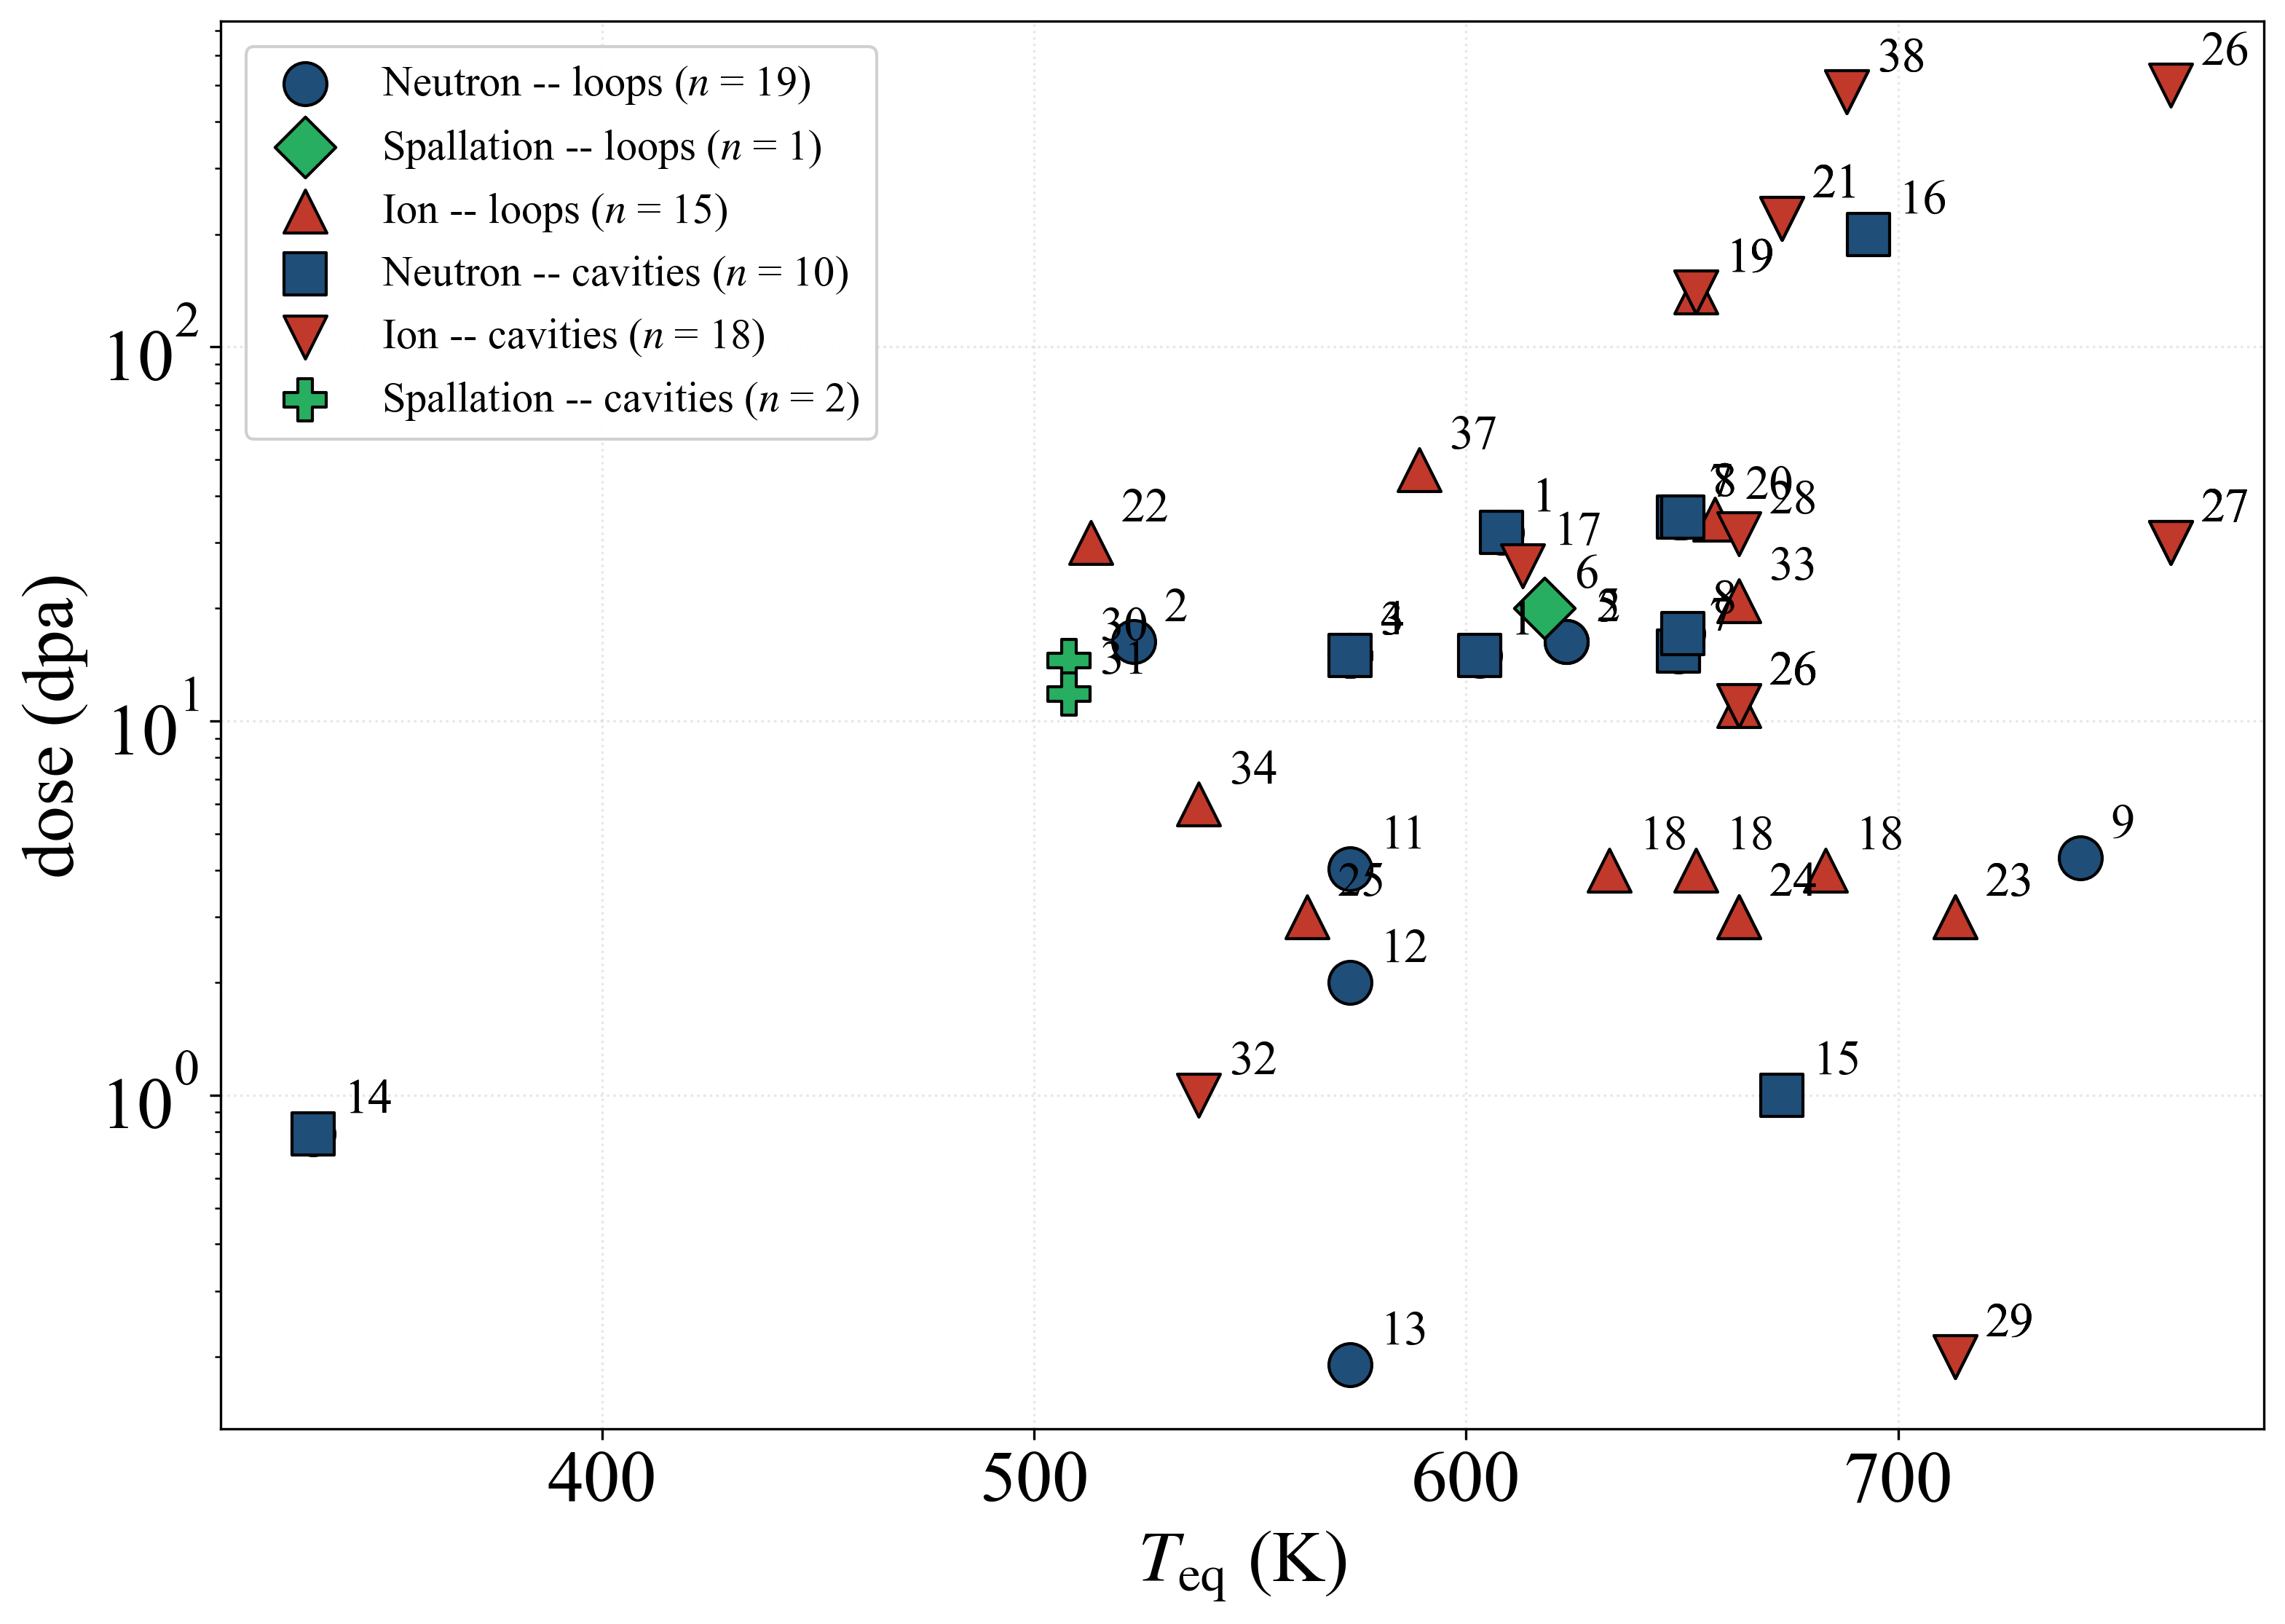
\includegraphics[width=\linewidth]{figures/experiments/coverage_dose_temperature.png}
  \caption{Coverage of the $(T_{\rm eq}, \text{dose})$ plane by the database.
  Colour encodes the irradiation class and marker shape the defect population;
  each point carries the number of the paper it was measured in
  (Table~\ref{tab:refs}). Neutron and ion data occupy different regions --- the
  neutron set extends to $333$~K but only to $35$~dpa, the ion set begins at
  $513$~K and reaches $650$~dpa --- which is why the two are fitted separately
  throughout this section.}
  \label{fig:coverage}
\end{figure}

\begin{table}[htbp]
\centering\small
\caption{Sources of the database rows. The number in the first column is the
label carried by every point measured in that paper, in every figure of this
section. A dagger marks an entry whose first author differs from the workbook's
author--year key (the key is retained because the database is indexed on it);
an asterisk marks an entry for which no published paper could be matched, and
for which no citation is therefore given. Sources 39--51, introduced by the
\texttt{Loop\_fractions} sheet, are listed separately in
Table~\ref{tab:lf-refs}.}
\label{tab:refs}
\begin{tabular}{rllrll}
\toprule
\# & Source & Reference & \# & Source & Reference \\
\midrule
 1 & Klimenkov 2012$^{\dagger}$    & JNM 426 (2012) 52      & 20 & Toloczko 2024$^{*}$        & --- \\
 2 & Gaganidze 2011                & JNM 417 (2011) 93      & 21 & Getto 2015                 & JNM 465 (2015) 116 \\
 3 & Gaganidze 2016$^{\dagger}$    & NME 9 (2016) 471       & 22 & Ando 2018$^{*}$            & --- \\
 4 & Dethloff 2016                 & NME 9 (2016) 471       & 23 & Swenson \& Wharry 2018     & JNM 502 (2018) 30 \\
 5 & Klimenkov 2017                & JNM 493 (2017) 426     & 24 & Jiang 2024$^{*}$           & --- \\
 6 & Wan 2010$^{*}$                & ---                    & 25 & Boulanger \& Serruys 2009  & JNM 386--388 (2009) 441 \\
 7 & Gao 2018$^{\dagger}$          & JNM 504 (2018) 122     & 26 & Liu 2023$^{*}$             & --- \\
 8 & Gao 2019$^{\dagger}$          & JNM 523 (2019) 421     & 27 & Song 2018                  & JNM 502 (2018) 76 \\
 9 & Zhong 2021                    & JNM 552 (2021) 153001  & 28 & Wakai 2002                 & JNM 307--311 (2002) 278 \\
10 & Zhong 2024                    & JNM 593 (2024) 154990  & 29 & Yutani 2007                & J. ASTM Int. 4 (2007) JAI100701 \\
11 & Yan 2021                      & JNM 557 (2021) 153207  & 30 & Dai 2004$^{*}$             & --- \\
12 & Lambrecht 2014$^{\dagger}$    & JNM 533 (2020) 152130  & 31 & Jia 2005                   & JNM 343 (2005) 212 \\
13 & Lambrecht 2009                & JNM 385 (2009) 334     & 32 & Schroeder \& Trinkaus 1986$^{\dagger}$ & JNM 141--143 (1986) 723 \\
14 & Eldrup 1999                   & JNM 271--272 (1999) 97 & 33 & Auger 2019$^{\dagger}$     & JNM 528 (2020) 151852 \\
15 & English 1982                  & JNM 108--109 (1982) 222& 34 & Rogozhkin 2020             & Inorg. Mater. Appl. Res. 11 (2020) 359 \\
16 & Gelles 1990s$^{*}$            & ---                    & 35 & Gilbon 1988                & JNM 155--157 (1988) 1268 \\
17 & Rouffi\'e 2014                & HAL cea-02383837       & 36 & Konstantinovic 2021$^{\dagger}$ & JNM 545 (2021) 152724 \\
18 & Zheng 2018                    & Phil.\ Mag.\ 98 (2018) 2440 & 37 & Was 2025              & JNM 616 (2025) 156065 \\
19 & Toloczko 2015$^{\dagger}$     & JNM 462 (2015) 458     & 38 & Lee 2021$^{*}$             & --- \\
\bottomrule
\end{tabular}
\end{table}


\subsection{Neutron irradiation}
\label{sec:expdb:neutron}

The neutron set comprises $19$ loop rows and $7$ fitted cavity rows (plus one
loop and two cavity rows from spallation, plotted but not fitted), covering
$T_{\rm eq} = 333$--$742$~K and $0.19$--$35.1$~dpa, in EUROFER97, EUROFER-ODS,
F82H, T91, HT9, Fe-9Cr and pure Fe.

\subsubsection{Loop number density}

Figure~\ref{fig:n-ld-T} shows the loop number density against $T_{\rm eq}$ and
Figure~\ref{fig:n-ld-invT} the same data on the Arrhenius axis. The result is a
negative one: over $400$~K of temperature the fitted slope is
$b = -9.3\times10^{-4} \pm 3.6\times10^{-3}$~K$^{-1}$
($t = -0.26$, $R^{2} = 0.004$), and the Arrhenius form gives
$E_{\rm eff} = -0.044 \pm 0.074$~eV --- consistent with zero on both axes. None
of the eight candidate groupings lowers the LOO error meaningfully: the best,
a dose threshold at $15$~dpa, reaches $\mathrm{LOO} = 1.318$ against $1.368$ for
the temperature-only model at $p = 0.09$, and the alloy family, ODS flag and Cr
content are all worse than doing nothing (Table~\ref{tab:selection}). Markers in
Figure~\ref{fig:n-ld-T} are coloured by alloy family for information only; a
single line is fitted.

The honest summary of this panel is therefore a distribution rather than a trend:
\begin{equation}
  N_{\ell}^{\rm (n)} \;=\; 5.2\times10^{21}~\mathrm{m^{-3}}, \qquad
  \mathrm{GSD} = 3.3,
  \label{eq:nld}
\end{equation}
i.e.\ two thirds of all reported neutron loop densities lie between
$1.6\times10^{21}$ and $1.7\times10^{22}$~m$^{-3}$, and $95\,\%$ within a
factor $\mathrm{GSD}^{2} = 10.9$ of it. The spread is real and physical: it mixes
alloys, doses from $0.19$ to $35$~dpa, four reactors and a range of TEM
visibility thresholds, and the last of these alone can move a reported loop
density by an order of magnitude. A cluster-dynamics calculation that lands
anywhere inside Eq.~\eqref{eq:nld} is consistent with the neutron database; the
database cannot discriminate more finely than that.

\begin{figure}[htbp]
  \centering
  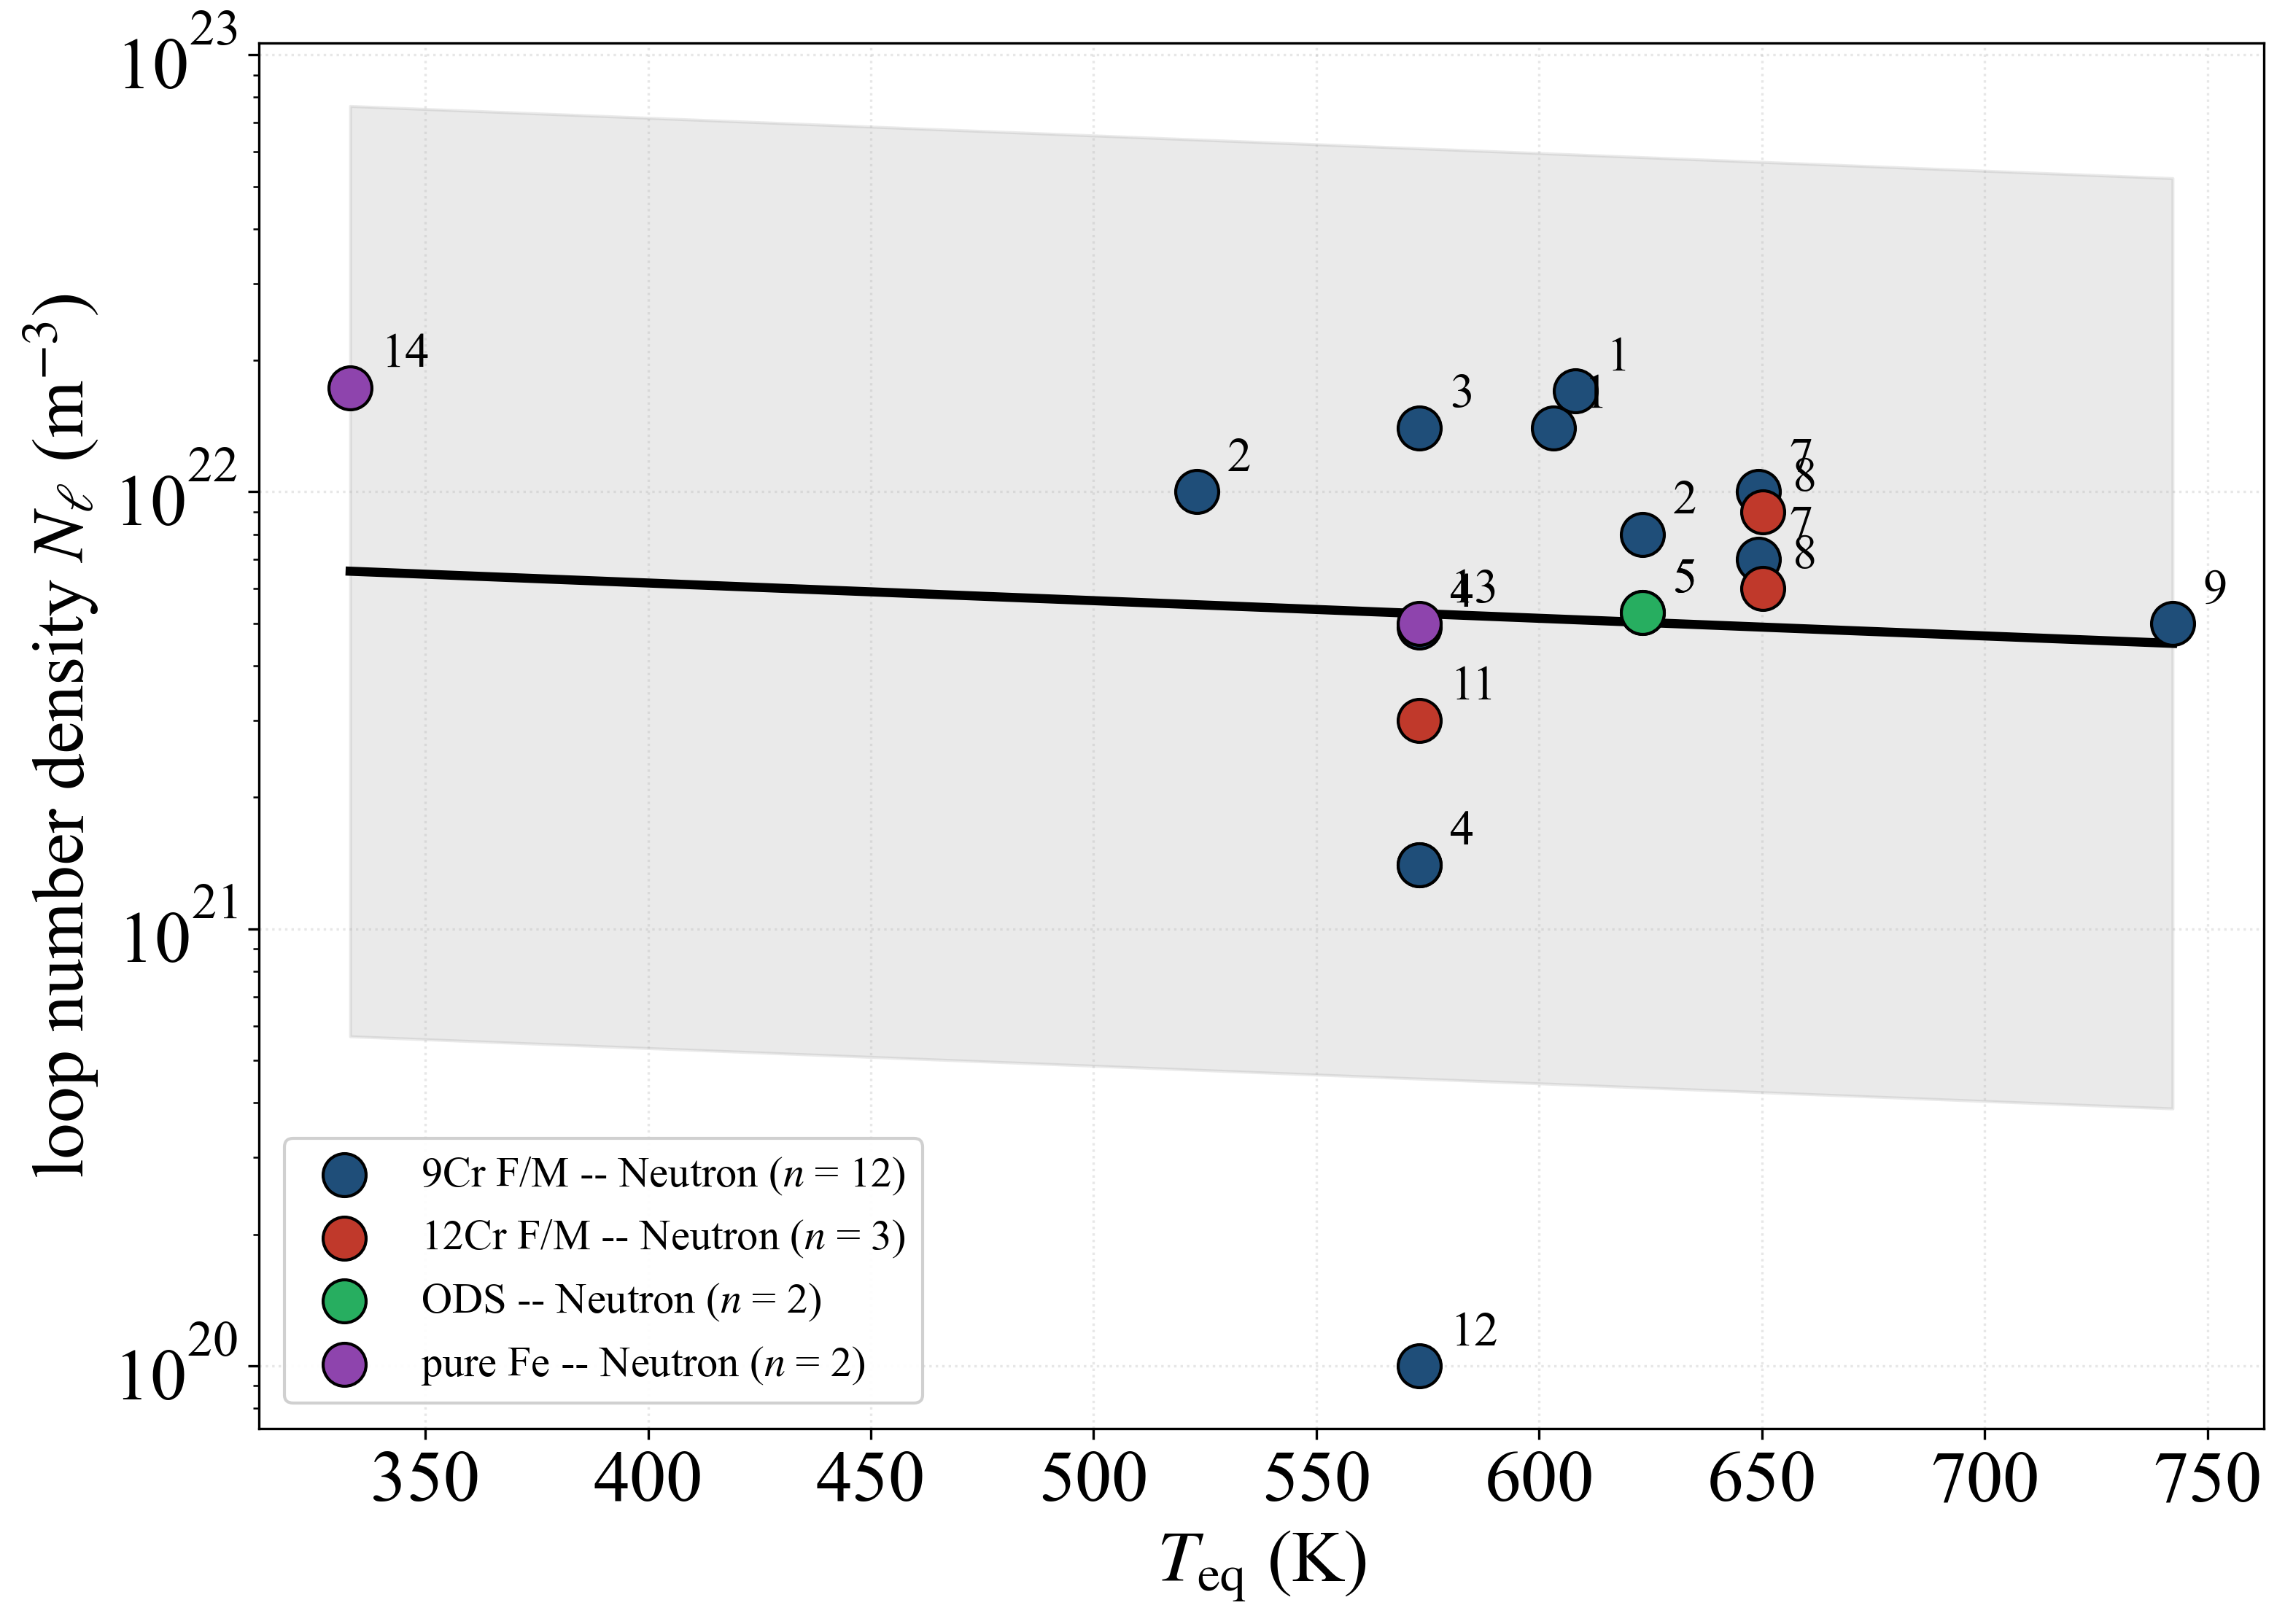
\includegraphics[width=\linewidth]{figures/experiments/neutron_loop_density_T.png}
  \caption{Neutron-irradiation loop number density against equivalent
  temperature. Marker colour is the alloy family and marker shape the irradiation
  class ($\bullet$ neutron, $\blacklozenge$ spallation); labels are the source
  numbers of Table~\ref{tab:refs}. The solid line is the log-linear fit to the
  $19$ neutron rows and the grey band the $\pm 2s$ ($\approx\!95\,\%$)
  log-normal prediction band. The fitted slope is not distinguishable from zero;
  the colouring by alloy family is descriptive, since no grouping tested reduces
  the leave-one-out error (Table~\ref{tab:selection}).}
  \label{fig:n-ld-T}
\end{figure}

\begin{figure}[htbp]
  \centering
  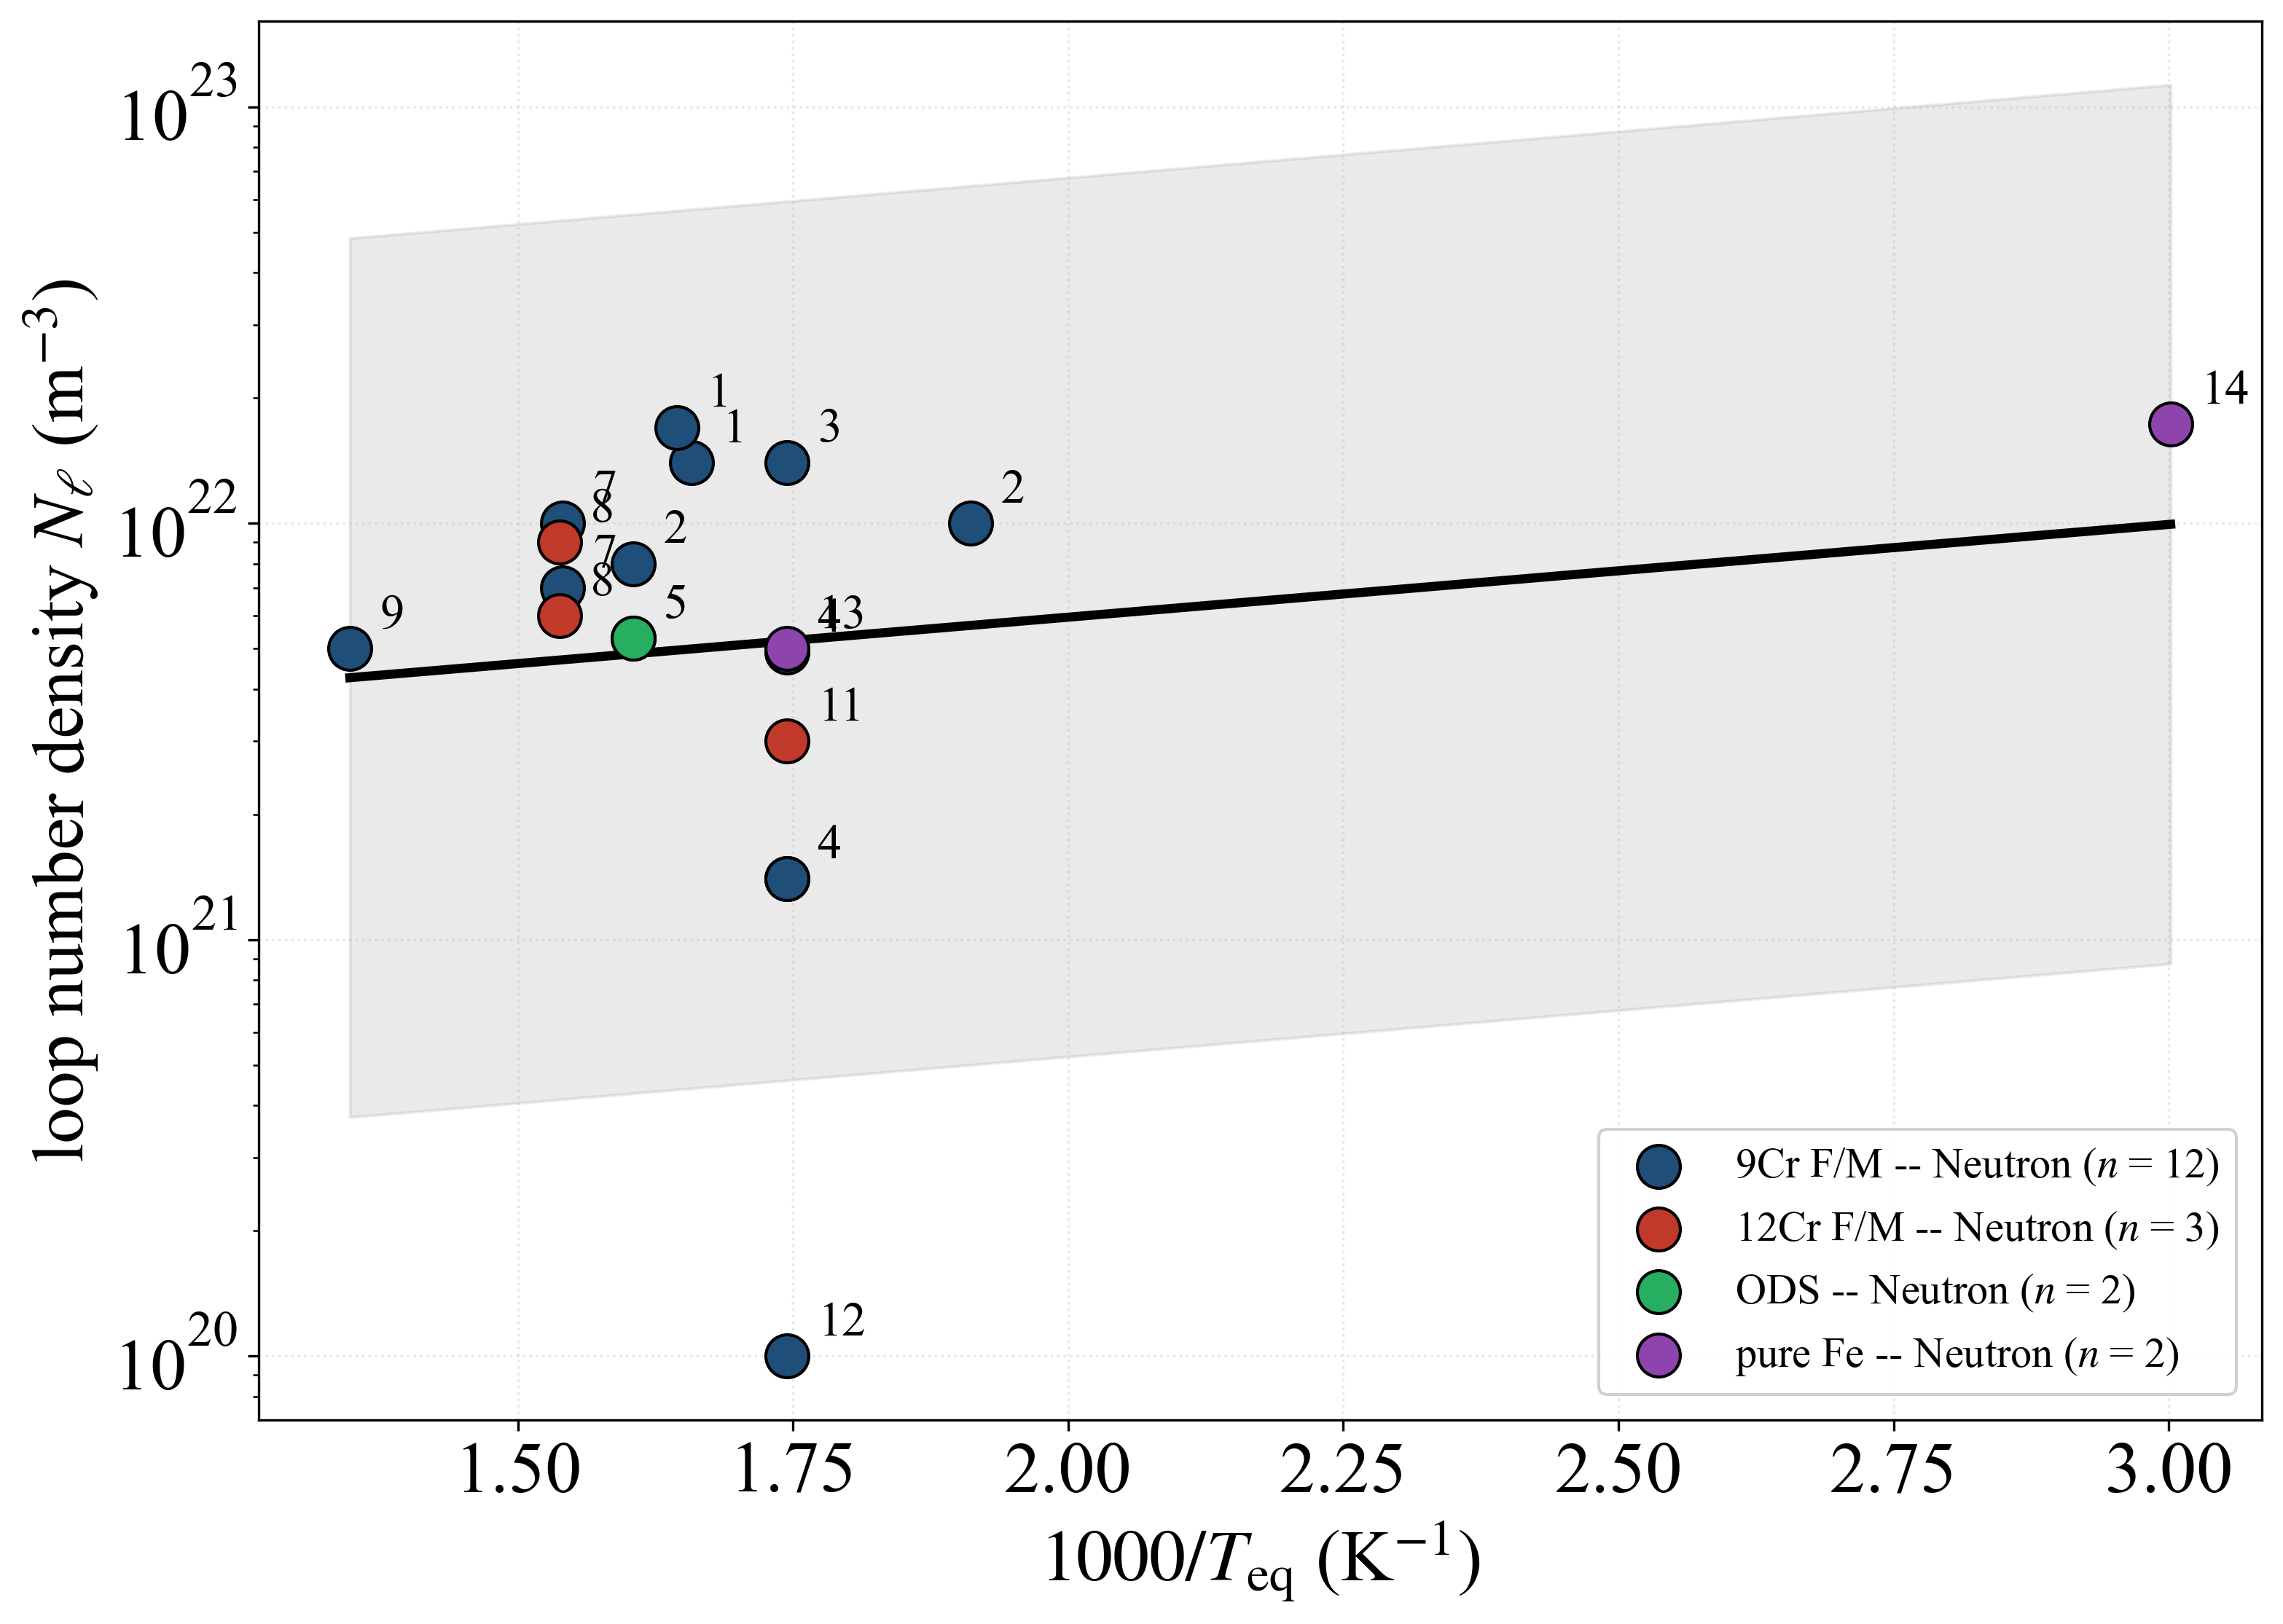
\includegraphics[width=\linewidth]{figures/experiments/neutron_loop_density_invT.png}
  \caption{The data of Figure~\ref{fig:n-ld-T} on the Arrhenius axis. The
  effective activation energy, $E_{\rm eff} = -0.044 \pm 0.074$~eV, is consistent
  with zero: within the scatter of the pooled neutron database the loop number
  density carries no measurable thermal activation.}
  \label{fig:n-ld-invT}
\end{figure}

\subsubsection{Mean loop diameter}

The loop size panel is the one place in the neutron data where a grouping is
clearly justified. The coarse alloy family lowers the LOO error from $0.746$ to
$0.569$ and the residual variance from $s^{2} = 0.394$ to $0.178$ --- $55\,\%$
of the variance in $\ln \bar d$ removed --- at a nested-$F$ probability of
$p = 0.0025$ (Table~\ref{tab:selection}). With a common slope
$b = 2.82\times10^{-3} \pm 1.62\times10^{-3}$~K$^{-1}$ the group offsets relative
to 9Cr F/M are, in Figure~\ref{fig:n-ls-T},
\begin{equation}
  \begin{aligned}
    c_{\rm 12Cr\ F/M} &= +0.87 \pm 0.27 \quad (\times 2.4,\ t = +3.2), \\
    c_{\rm ODS}       &= +1.19 \pm 0.32 \quad (\times 3.3,\ t = +3.7), \\
    c_{\rm pure\ Fe}  &= +0.92 \pm 0.41 \quad (\times 2.5,\ t = +2.3),
  \end{aligned}
  \label{eq:nls}
\end{equation}
so at $600$~K the fit predicts $\bar d_{\ell} \approx 6$~nm in 9Cr F/M steels
against $\approx 14$~nm in 12Cr grades, $\approx 15$~nm in pure Fe and
$\approx 20$~nm in the ODS variants, with a residual scatter of
$\mathrm{GSD} = 1.53$ about each line.

The ordering is physically coherent. In the 9Cr RAFM grades the high density of
Cr, C and N solutes and of $\rm M_{23}C_6$ interfaces traps migrating self-
interstitial clusters and truncates their growth, giving a dense population of
small loops; pure Fe, with none of that trapping, grows the same number of loops
to larger size. The offsets should nevertheless be read with the confounding in
mind: the ODS group is only two rows (EUROFER-ODS at $16.3$~dpa, both at
$623$~K), and both were imaged in one study, so $c_{\rm ODS}$ carries the
between-laboratory difference as well as the alloy effect. The slope itself is
only $1.7\sigma$ from zero, so the temperature dependence of the mean loop
diameter remains weakly determined even after grouping --- what the grouping
buys is a much tighter prediction band, not a better-resolved trend.

\begin{figure}[htbp]
  \centering
  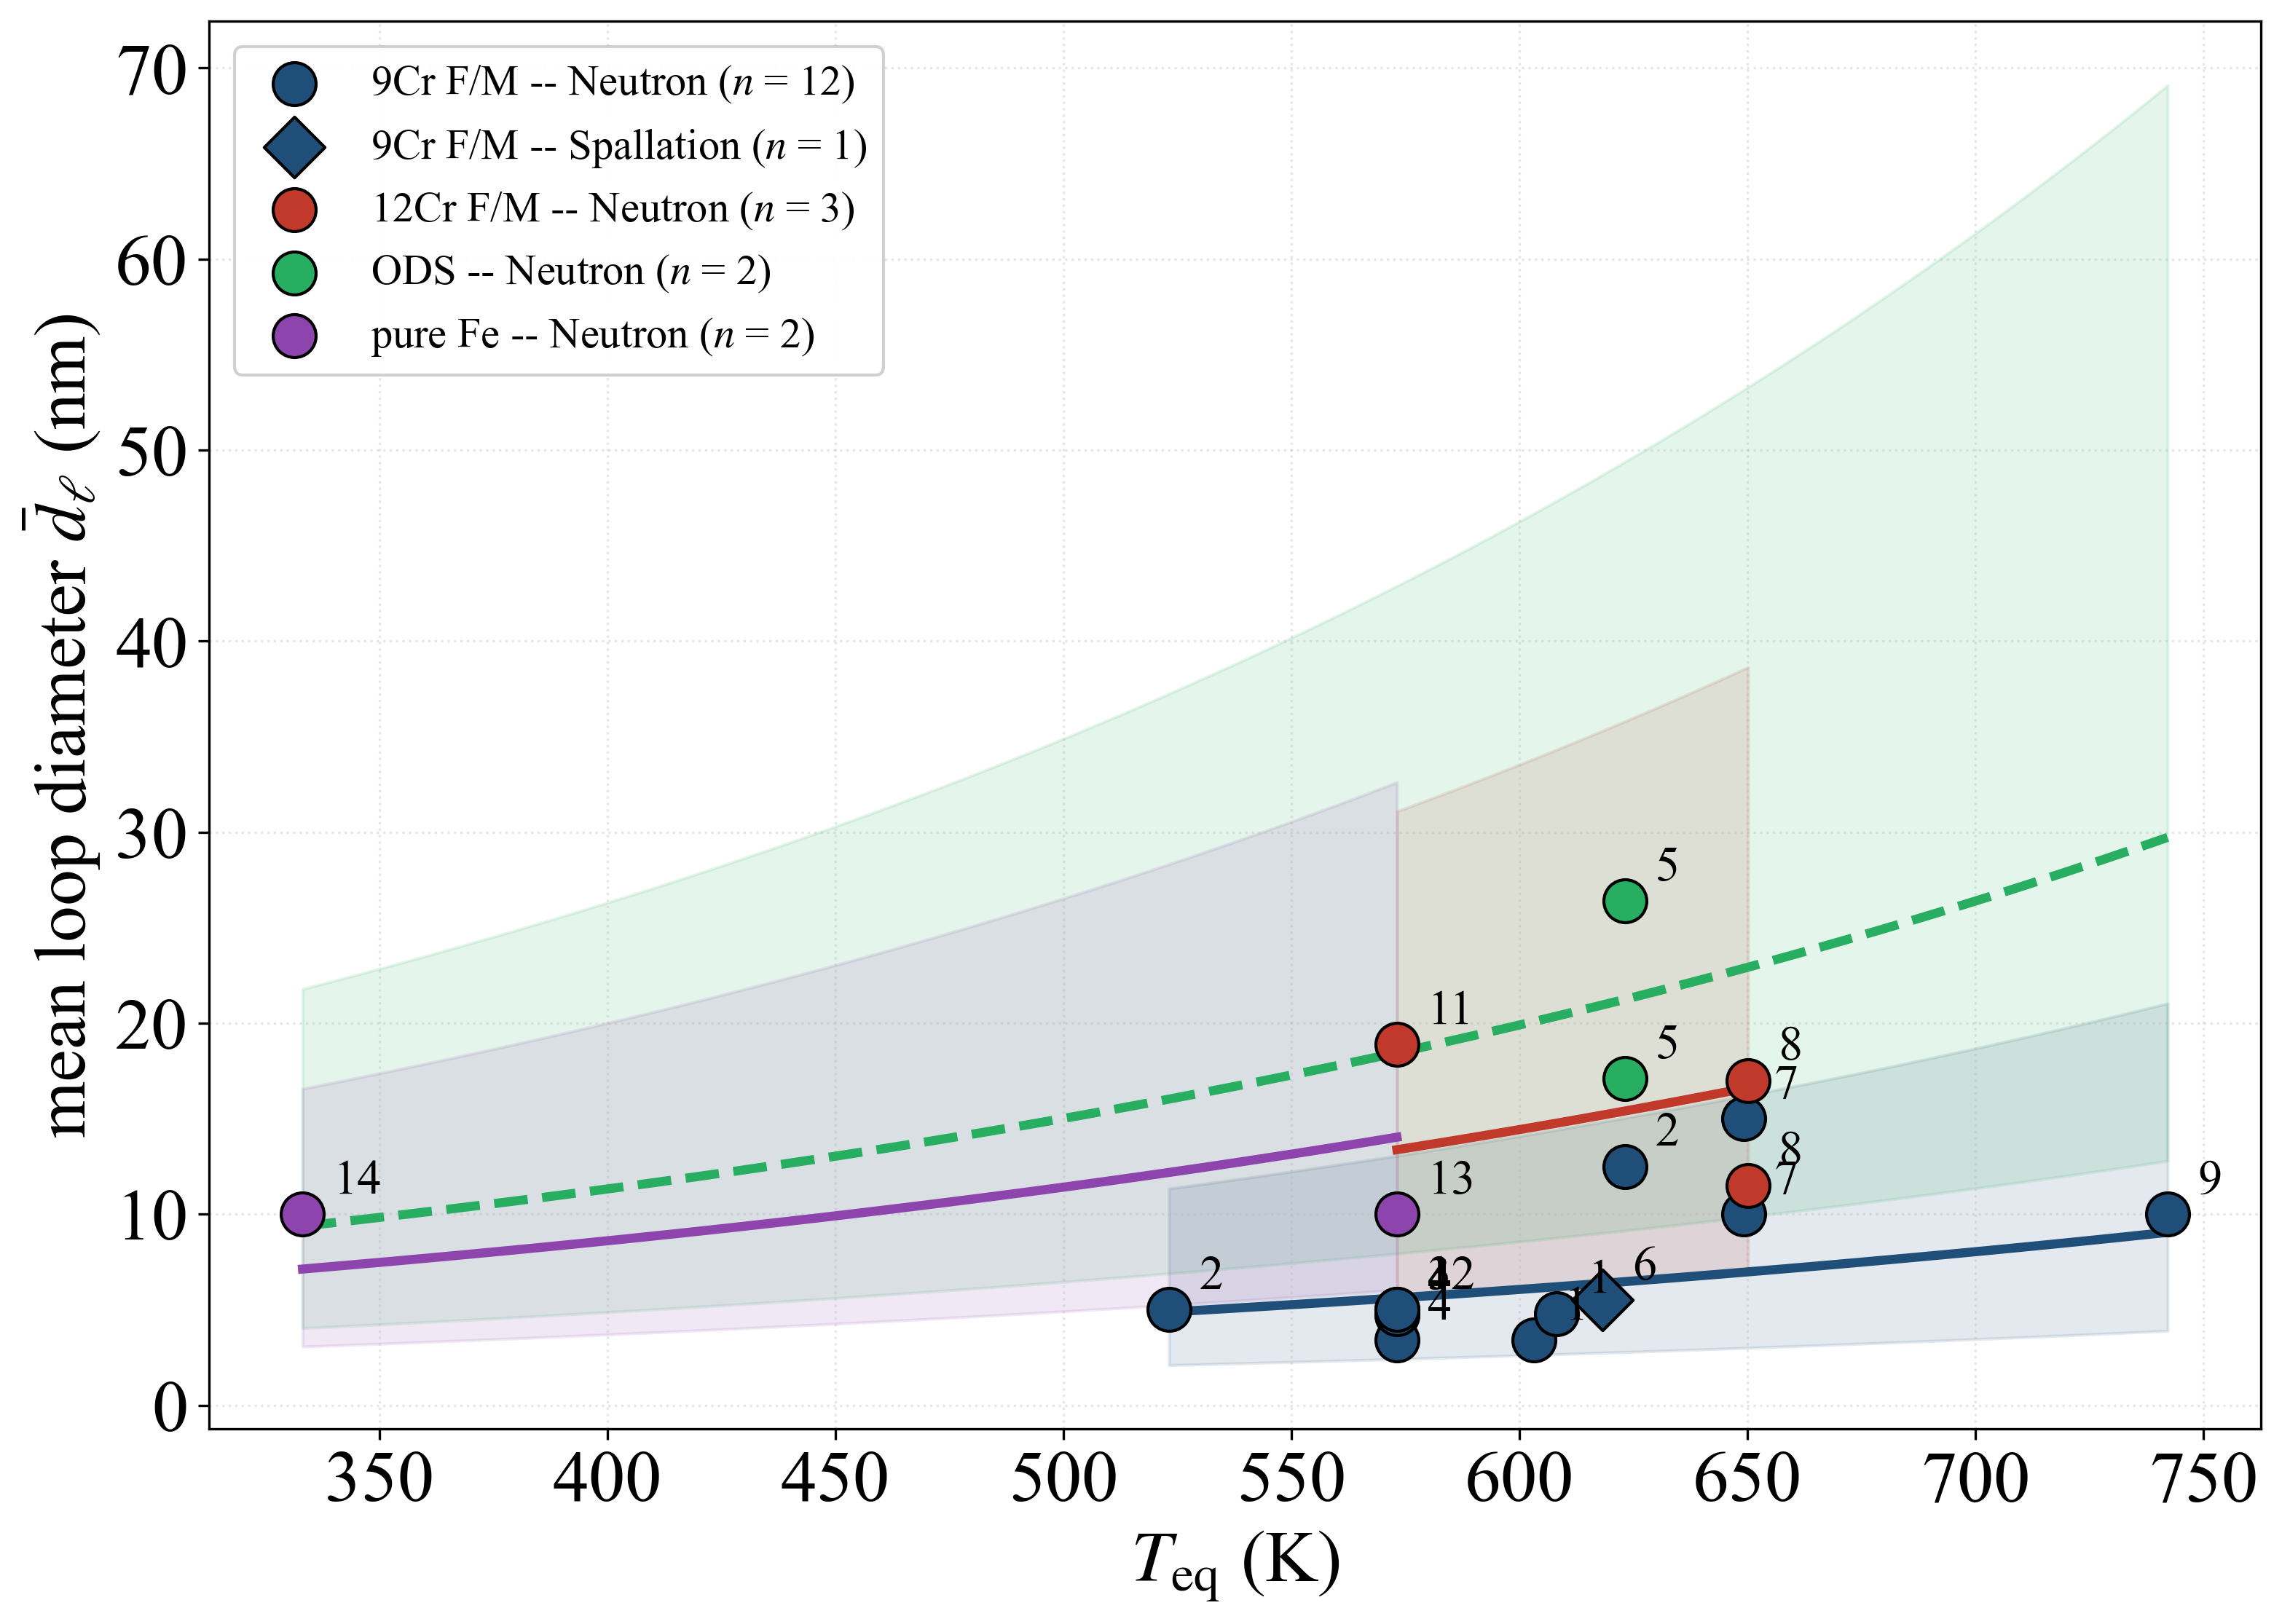
\includegraphics[width=\linewidth]{figures/experiments/neutron_loop_size_T.png}
  \caption{Neutron-irradiation mean loop diameter against equivalent temperature,
  grouped by alloy family with a common temperature slope and group-specific
  intercepts. Bands are the $\pm 2s$ prediction bands of the common-slope model.
  The ODS line is dashed because both ODS rows were measured at the same
  temperature. The spallation point (source 6, diamond) is plotted but not
  fitted. Grouping by family removes $55\,\%$ of
  the variance in $\ln \bar d$ ($p = 0.0025$).}
  \label{fig:n-ls-T}
\end{figure}

\subsubsection{Cavity number density}

The neutron cavity data are the sparsest panel in the database --- seven fitted
rows --- and they produce the steepest apparent trend anywhere in this section:
$b = -1.91\times10^{-2} \pm 3.4\times10^{-3}$~K$^{-1}$ ($t = -5.6$,
$R^{2} = 0.863$), equivalently $E_{\rm eff} = -0.364 \pm 0.053$~eV on the
Arrhenius axis (Figures~\ref{fig:n-cd-T} and~\ref{fig:n-cd-invT}). The fit
predicts $5\times10^{23}$~m$^{-3}$ at $350$~K falling to $4\times10^{21}$~m$^{-3}$
at $600$~K.

That trend must not be quoted without its leverage caveat. Two of the seven rows
are pure iron --- Eldrup 1999 at $333$~K, $0.79$~dpa
($1\times10^{24}$~m$^{-3}$, a positron-annihilation measurement of nanovoids) and
English 1982 at $673$~K, $1$~dpa --- and they alone span $340$~K of the
$400$~K lever arm. The remaining five rows are all F/M steels confined to
$603$--$650$~K, and fitted on their own they give
$b = +2.3\times10^{-2}$~K$^{-1}$: the slope \emph{reverses sign}. The apparent
strong temperature dependence of the neutron cavity density is thus a statement
about the difference between low-temperature pure iron and F/M steel at
$600$--$650$~K, not a temperature trend measured within either. Used as a
validation target it constrains only the endpoints; within the F/M steel window
the data support no more than a constant $\approx 2\times10^{21}$--$6\times10^{21}$~m$^{-3}$.

\begin{figure}[htbp]
  \centering
  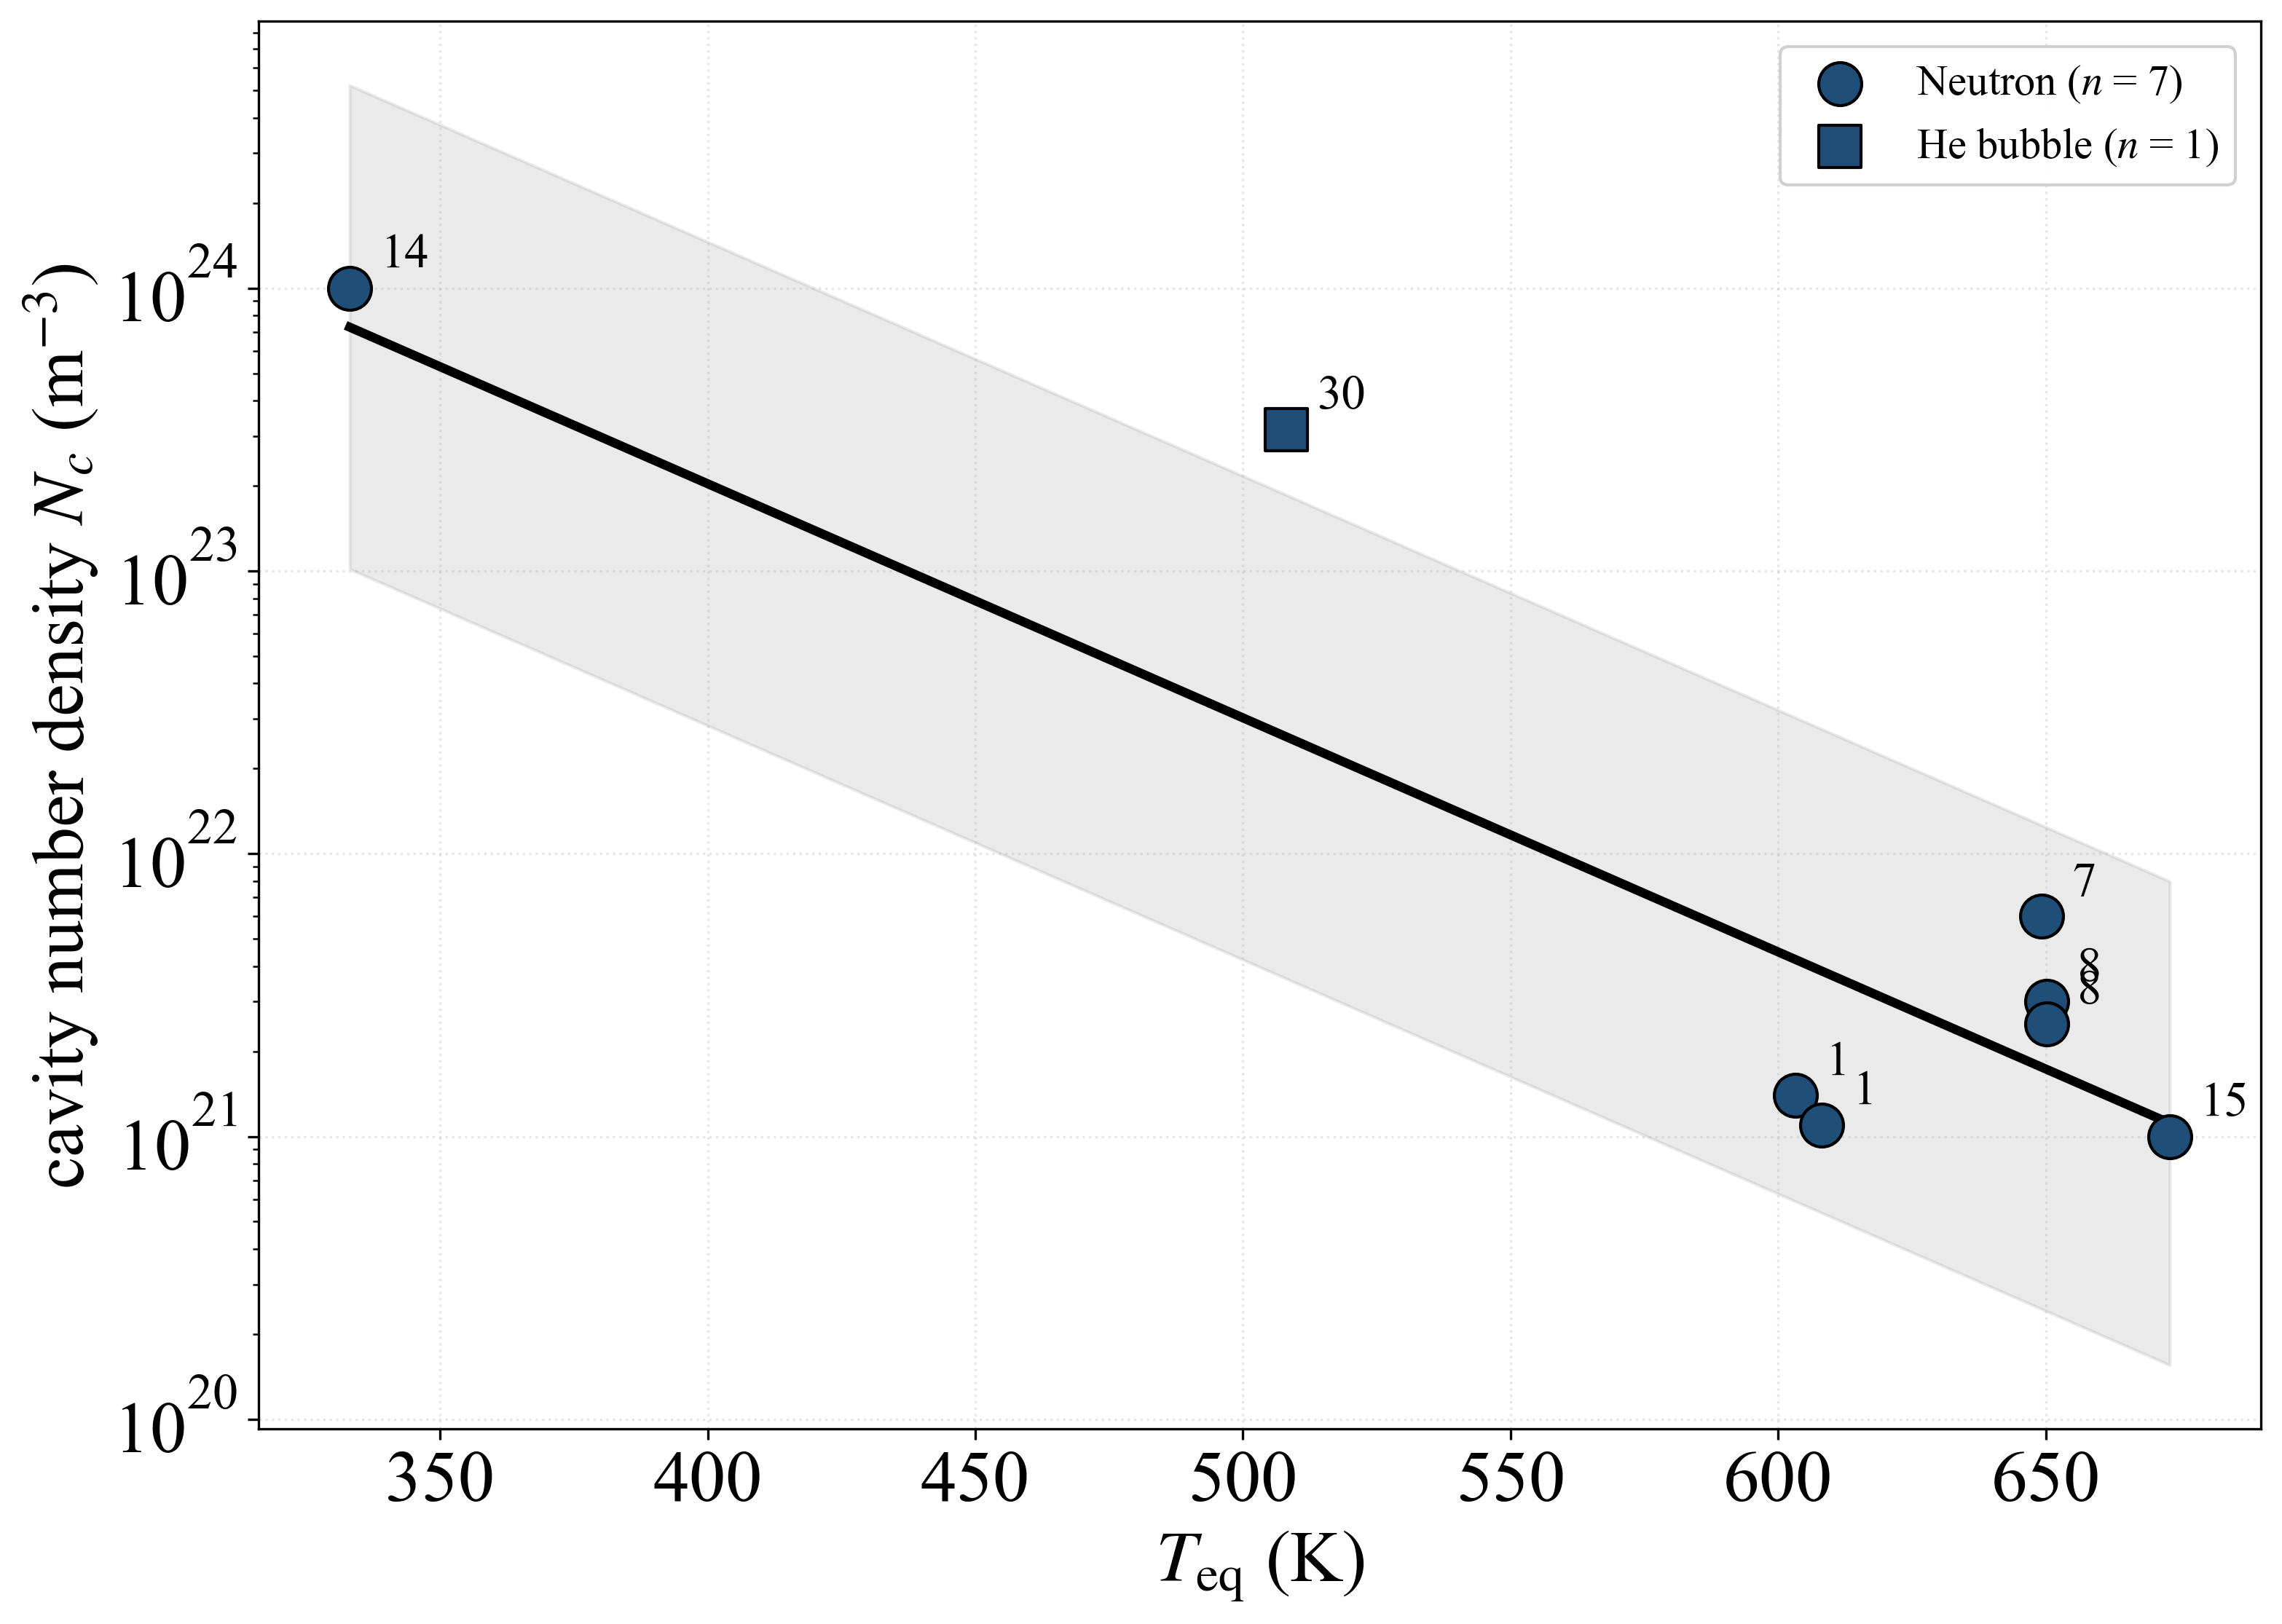
\includegraphics[width=\linewidth]{figures/experiments/neutron_cavity_density_T.png}
  \caption{Neutron-irradiation cavity number density against equivalent
  temperature, with the log-linear fit and its $\pm 2s$ prediction band. The
  spallation point (source 30) is plotted but not fitted. The steep negative
  slope rests on the two pure-Fe rows (sources 14 and 15) at the extremes of the
  temperature range; the five F/M-steel rows alone, spanning only $603$--$650$~K,
  give a slope of the opposite sign.}
  \label{fig:n-cd-T}
\end{figure}

\begin{figure}[htbp]
  \centering
  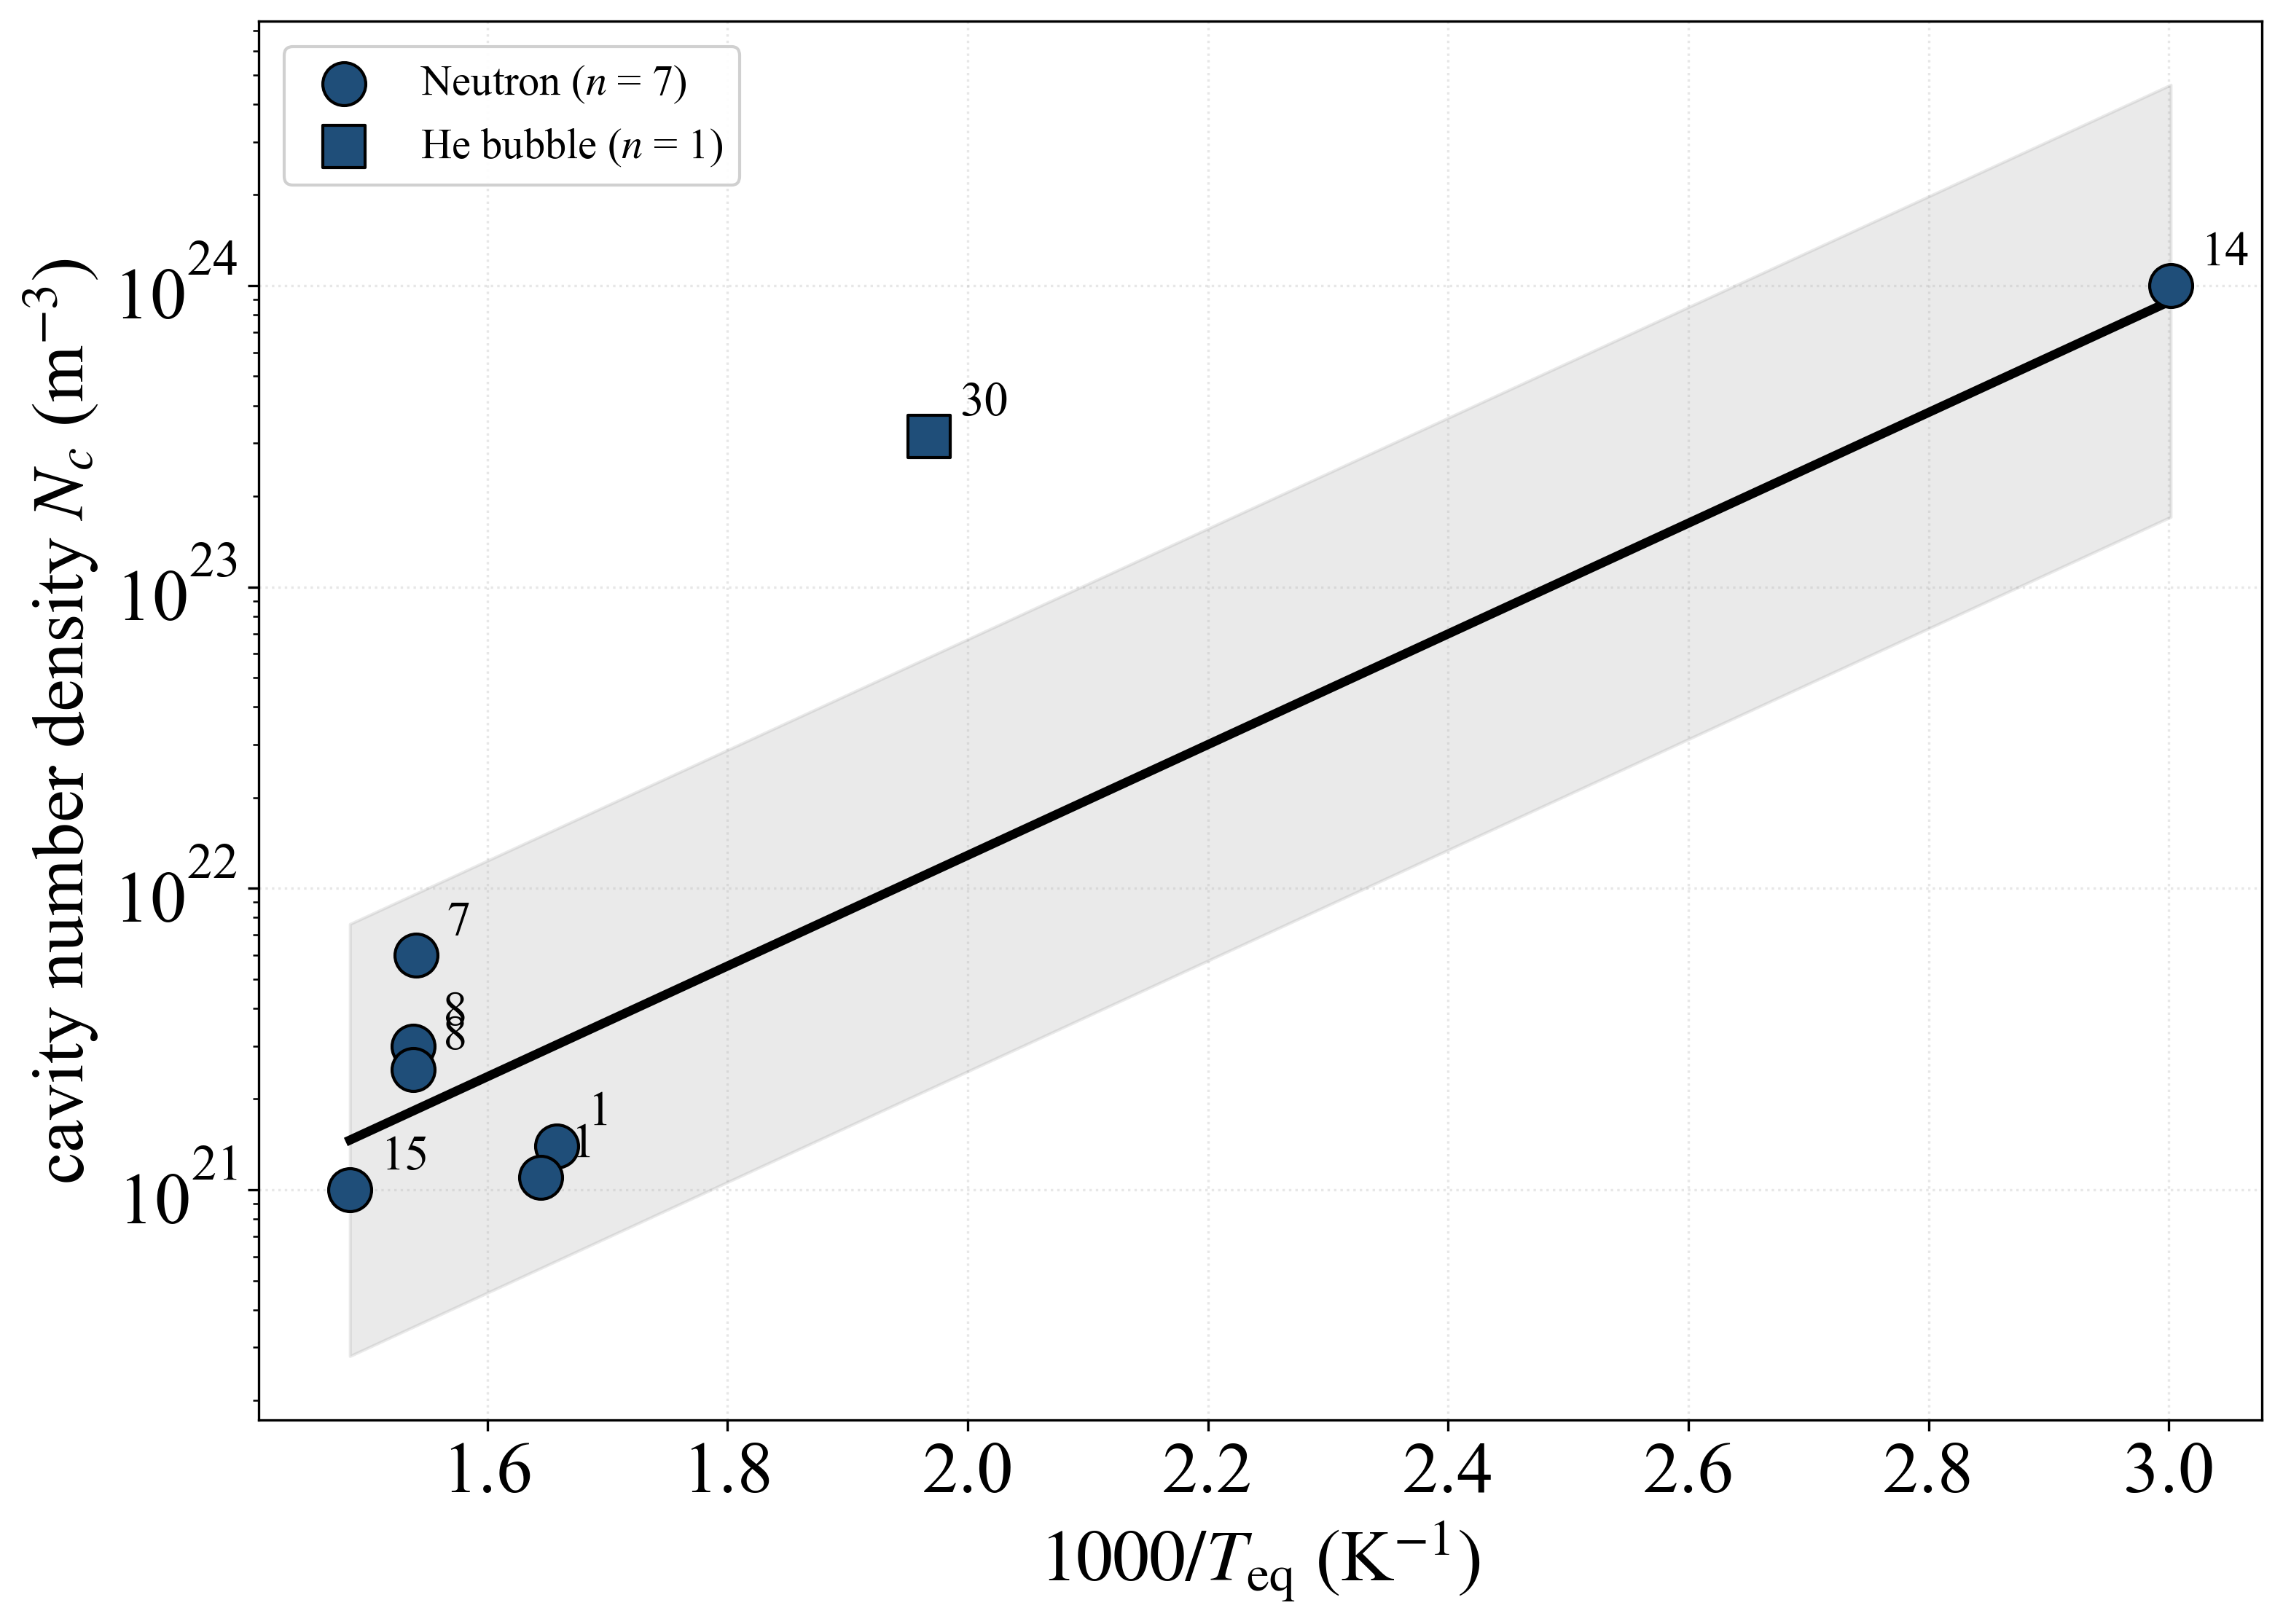
\includegraphics[width=\linewidth]{figures/experiments/neutron_cavity_density_invT.png}
  \caption{The data of Figure~\ref{fig:n-cd-T} on the Arrhenius axis,
  $E_{\rm eff} = -0.364 \pm 0.053$~eV. The same leverage caveat applies: the
  activation energy is set by the two pure-Fe endpoints.}
  \label{fig:n-cd-invT}
\end{figure}

\subsubsection{Mean cavity diameter}

The mean cavity diameter (Figure~\ref{fig:n-cs-T}) rises weakly with temperature,
$b = 3.14\times10^{-3} \pm 1.28\times10^{-3}$~K$^{-1}$ ($t = +2.5$,
$R^{2} = 0.545$, $\mathrm{GSD} = 1.44$), giving $\bar d_c \approx 2.3$~nm at
$600$~K. Cavities in neutron-irradiated F/M steel below $\sim\!700$~K are small
and dense: every EUROFER97, T91 and HT9 entry is at or below $2.6$~nm, several
reported only as $<2$~nm, and the bimodal T91 and HT9 rows at $35$~dpa report a
dominant small population plus a sparse large one. A dose split at $15$~dpa
appears to fit this panel spectacularly ($s^{2} = 0.018$, $R^{2} = 0.951$), but
it is not reported as a result: with seven points and the split falling between
rows at $15.0$ and $15.4$~dpa, the threshold was chosen by scanning and the
apparent gain is selection, not signal. As for the density, the trend is anchored
by the pure-Fe rows --- the five F/M rows alone give $R^{2} = 0.194$ with a slope
of opposite sign.

\begin{figure}[htbp]
  \centering
  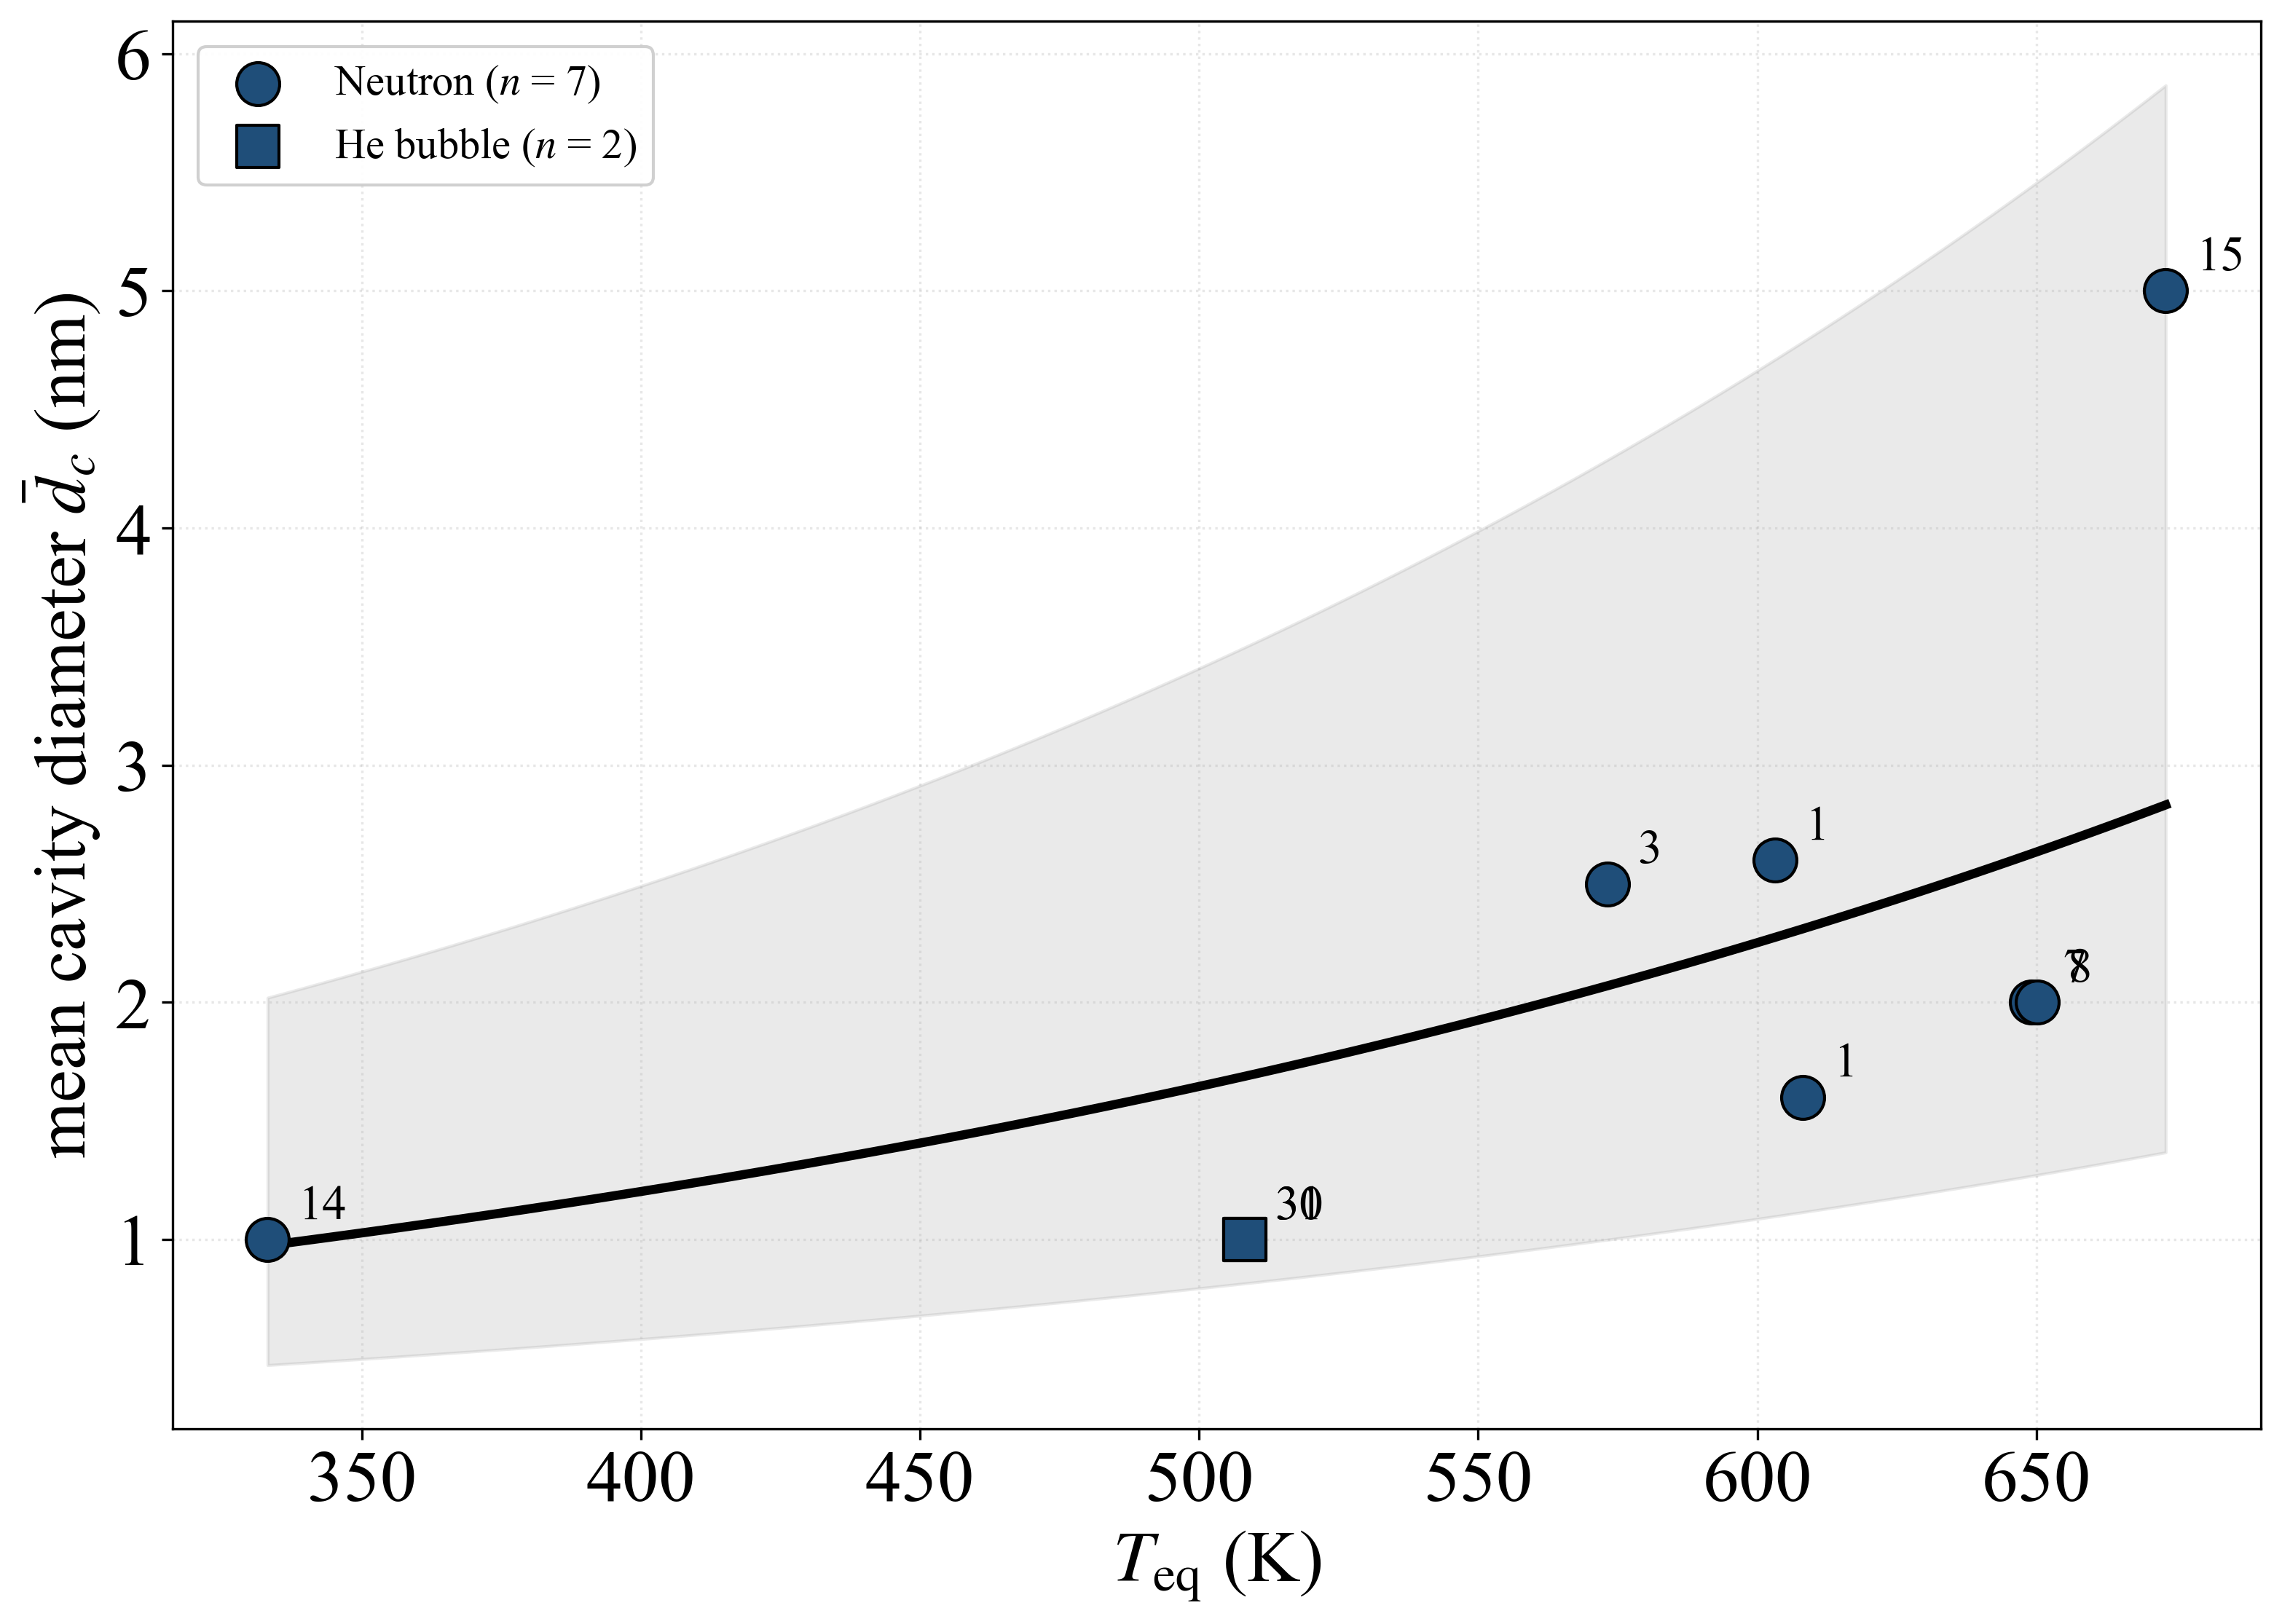
\includegraphics[width=\linewidth]{figures/experiments/neutron_cavity_size_T.png}
  \caption{Neutron-irradiation mean cavity diameter against equivalent
  temperature, with the log-linear fit and its $\pm 2s$ band. Spallation points
  (sources 30, 31) are plotted but not fitted. Cavities remain below $\sim 3$~nm
  throughout the F/M-steel window.}
  \label{fig:n-cs-T}
\end{figure}


\subsection{Ion irradiation}
\label{sec:expdb:ion}

The ion set comprises $10$ loop-density, $14$ loop-size, $12$ cavity-density and
$16$ fitted cavity-size rows over $T_{\rm eq} = 513$--$763$~K and
$0.2$--$650$~dpa. Its composition differs from the neutron set in three ways that
matter for the fits: the temperature range is narrower and higher, the dose range
is far wider, and roughly half the cavity rows are dual-beam or He-implantation
experiments in which the measured feature is a helium bubble, not a void.

\subsubsection{Loop number density}

Unlike the neutron panel, the ion loop density does respond to a grouping --- but
to dose, not to alloy. Splitting at $15$~dpa
(Figures~\ref{fig:i-ld-T} and~\ref{fig:i-ld-invT}) gives a common slope
$b = -2.32\times10^{-3} \pm 3.19\times10^{-3}$~K$^{-1}$, again indistinguishable
from zero, and an intercept offset
\begin{equation}
  c_{>15~\rm dpa} = -0.80 \pm 0.37 \quad (\times 0.45,\ t = -2.2),
  \label{eq:ild}
\end{equation}
so the loop density above $15$~dpa is about half that below it. This removes
$32\,\%$ of the variance at $p = 0.067$ and lowers the LOO error from $0.545$ to
$0.454$. Treating dose as a continuous covariate is marginally better still
($\mathrm{LOO} = 0.405$, $p = 0.024$, $s^{2} = 0.147$); the discrete split is
shown in the figure because it is directly comparable with the other panels of
this section, and both are reported in Table~\ref{tab:selection}.

A decreasing loop density with accumulated dose, at essentially constant loop
size, is the signature of loop coarsening and of loop absorption into the
dislocation network --- exactly the saturation mechanism that the loop--network
loss channel is intended to reproduce. It is worth noting how much tighter this
panel is than its neutron counterpart: $\mathrm{GSD} = 1.55$ about the fit
against $3.4$. Single-laboratory ion campaigns with consistent TEM protocols
scatter far less than a database assembled from twenty neutron studies, which is
an argument for using ion data to test trends and neutron data to test absolute
levels.

\begin{figure}[htbp]
  \centering
  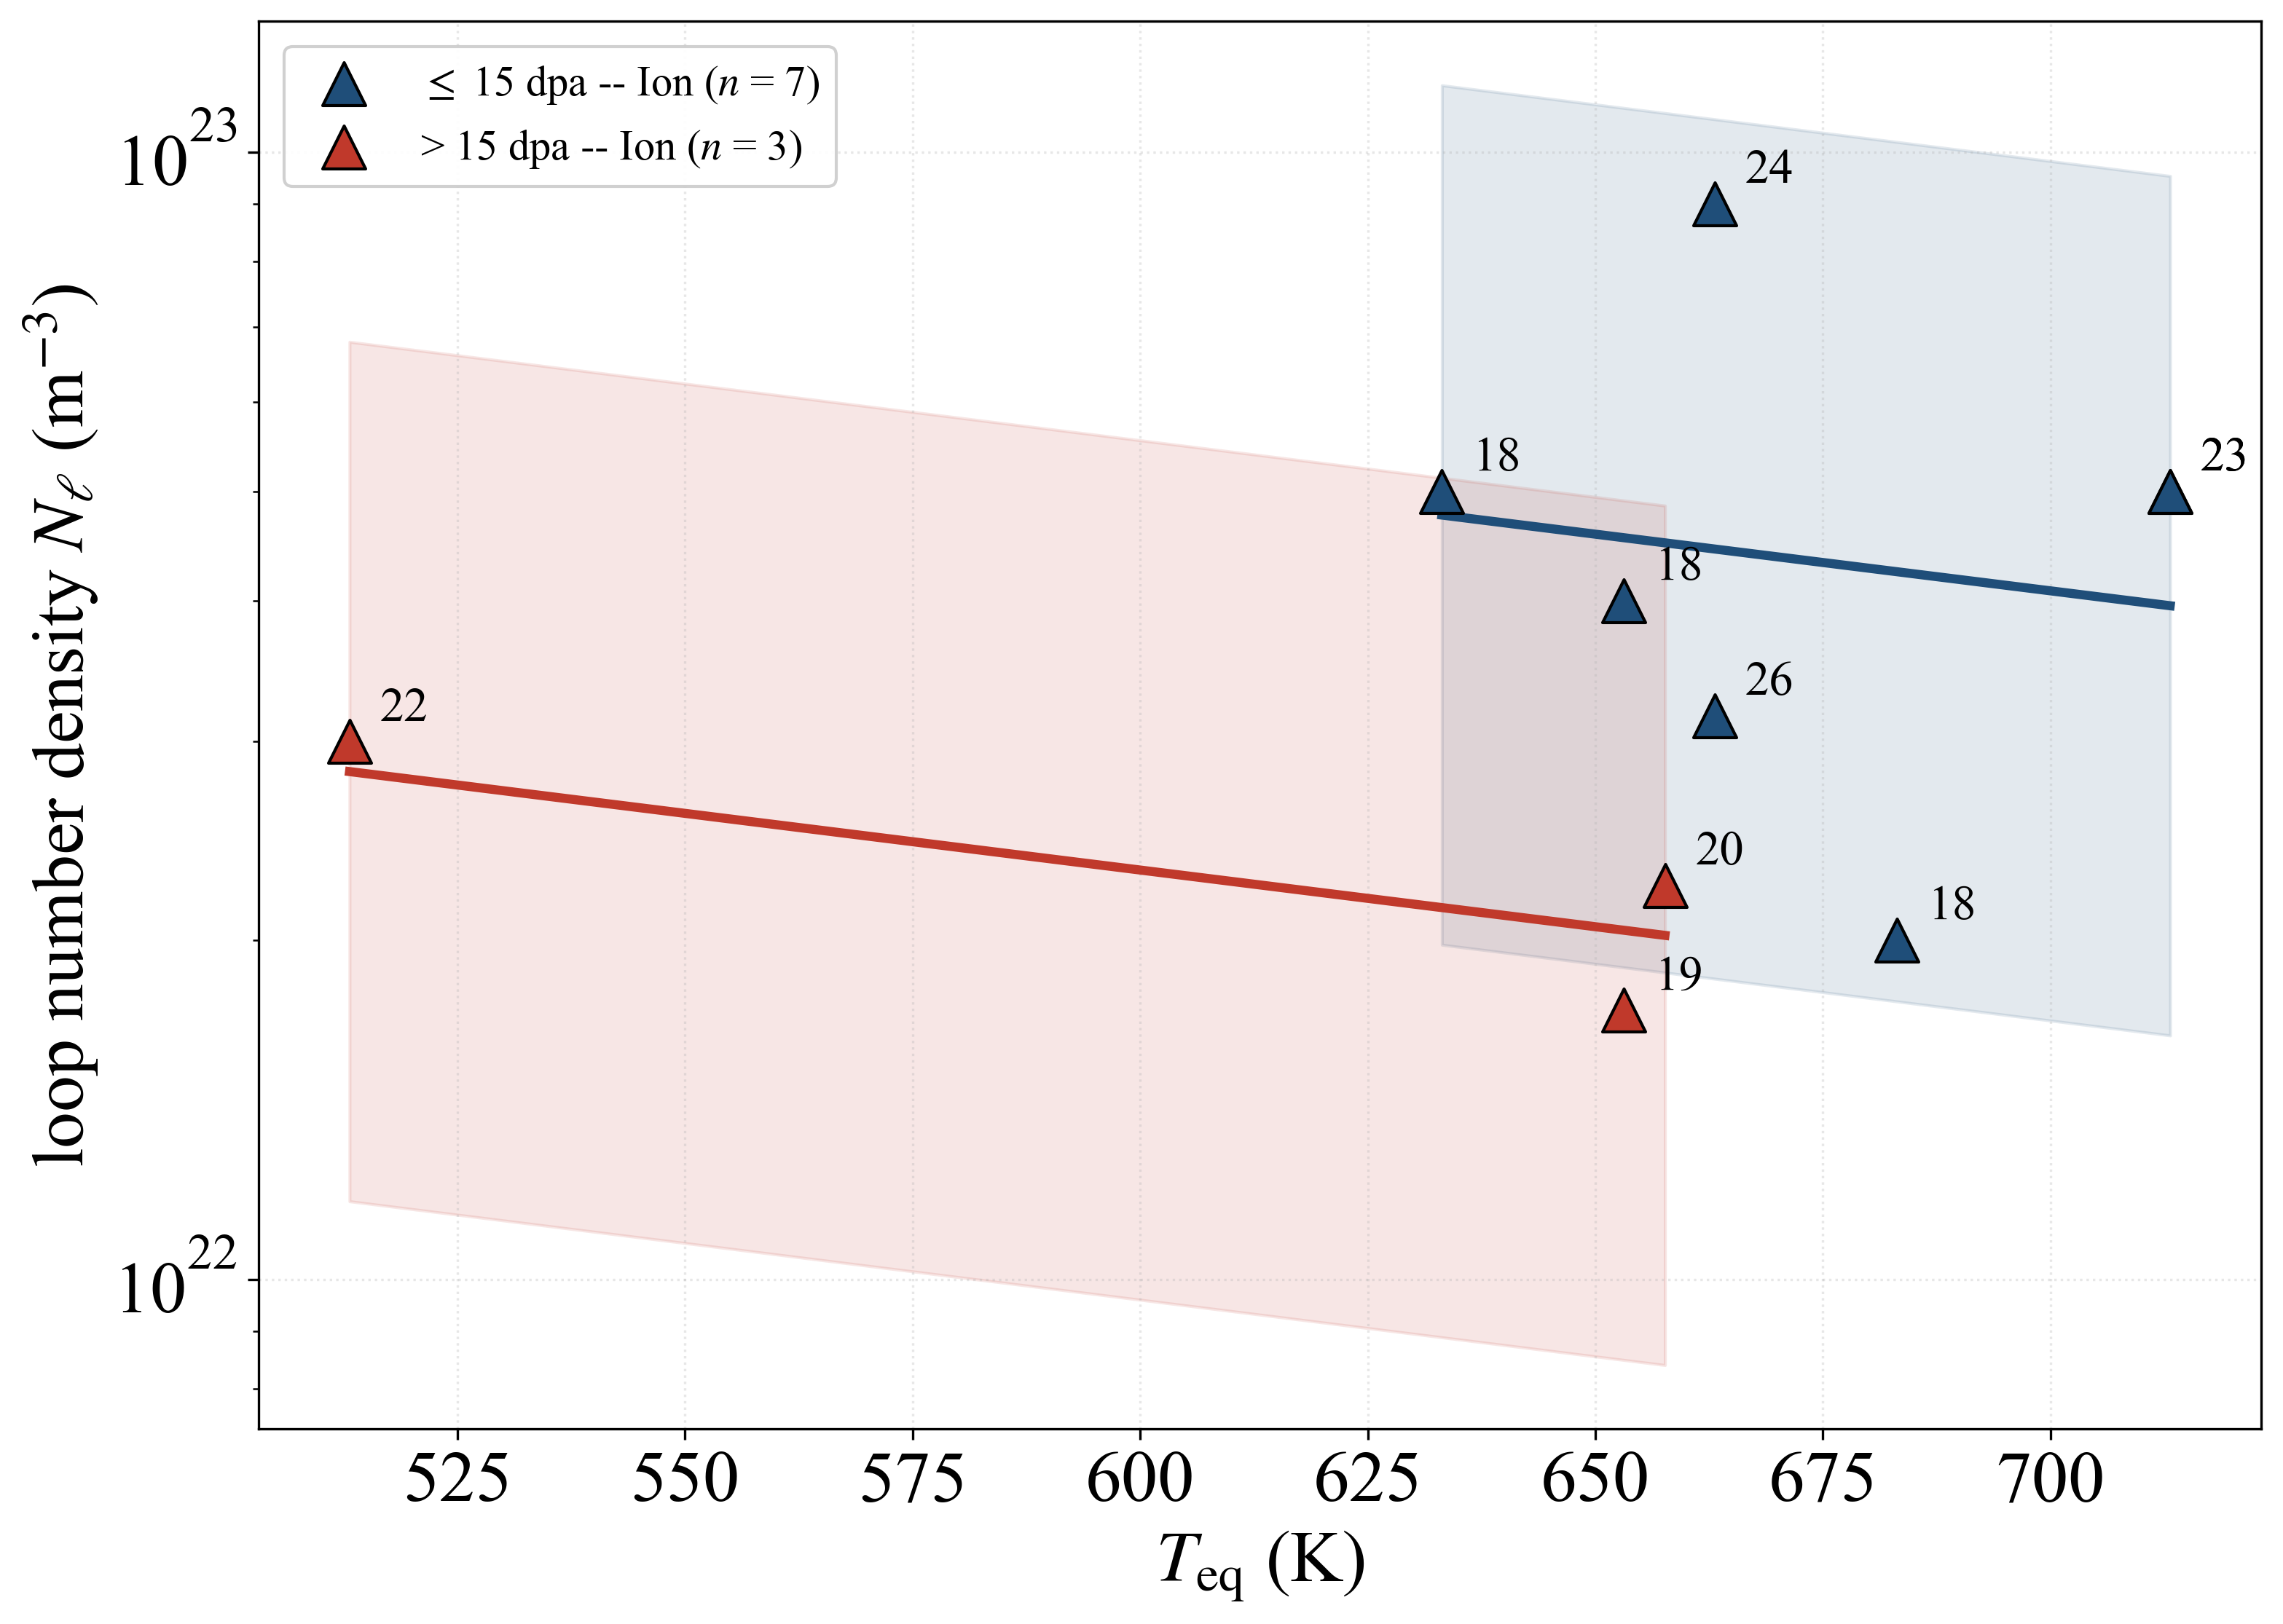
\includegraphics[width=\linewidth]{figures/experiments/ion_loop_density_T.png}
  \caption{Ion-irradiation loop number density against equivalent temperature,
  grouped at $15$~dpa with a common temperature slope. Bands are the $\pm 2s$
  prediction bands. Above $15$~dpa the loop density is a factor $\approx 0.45$
  below the low-dose group; the temperature slope itself is not resolved.}
  \label{fig:i-ld-T}
\end{figure}

\begin{figure}[htbp]
  \centering
  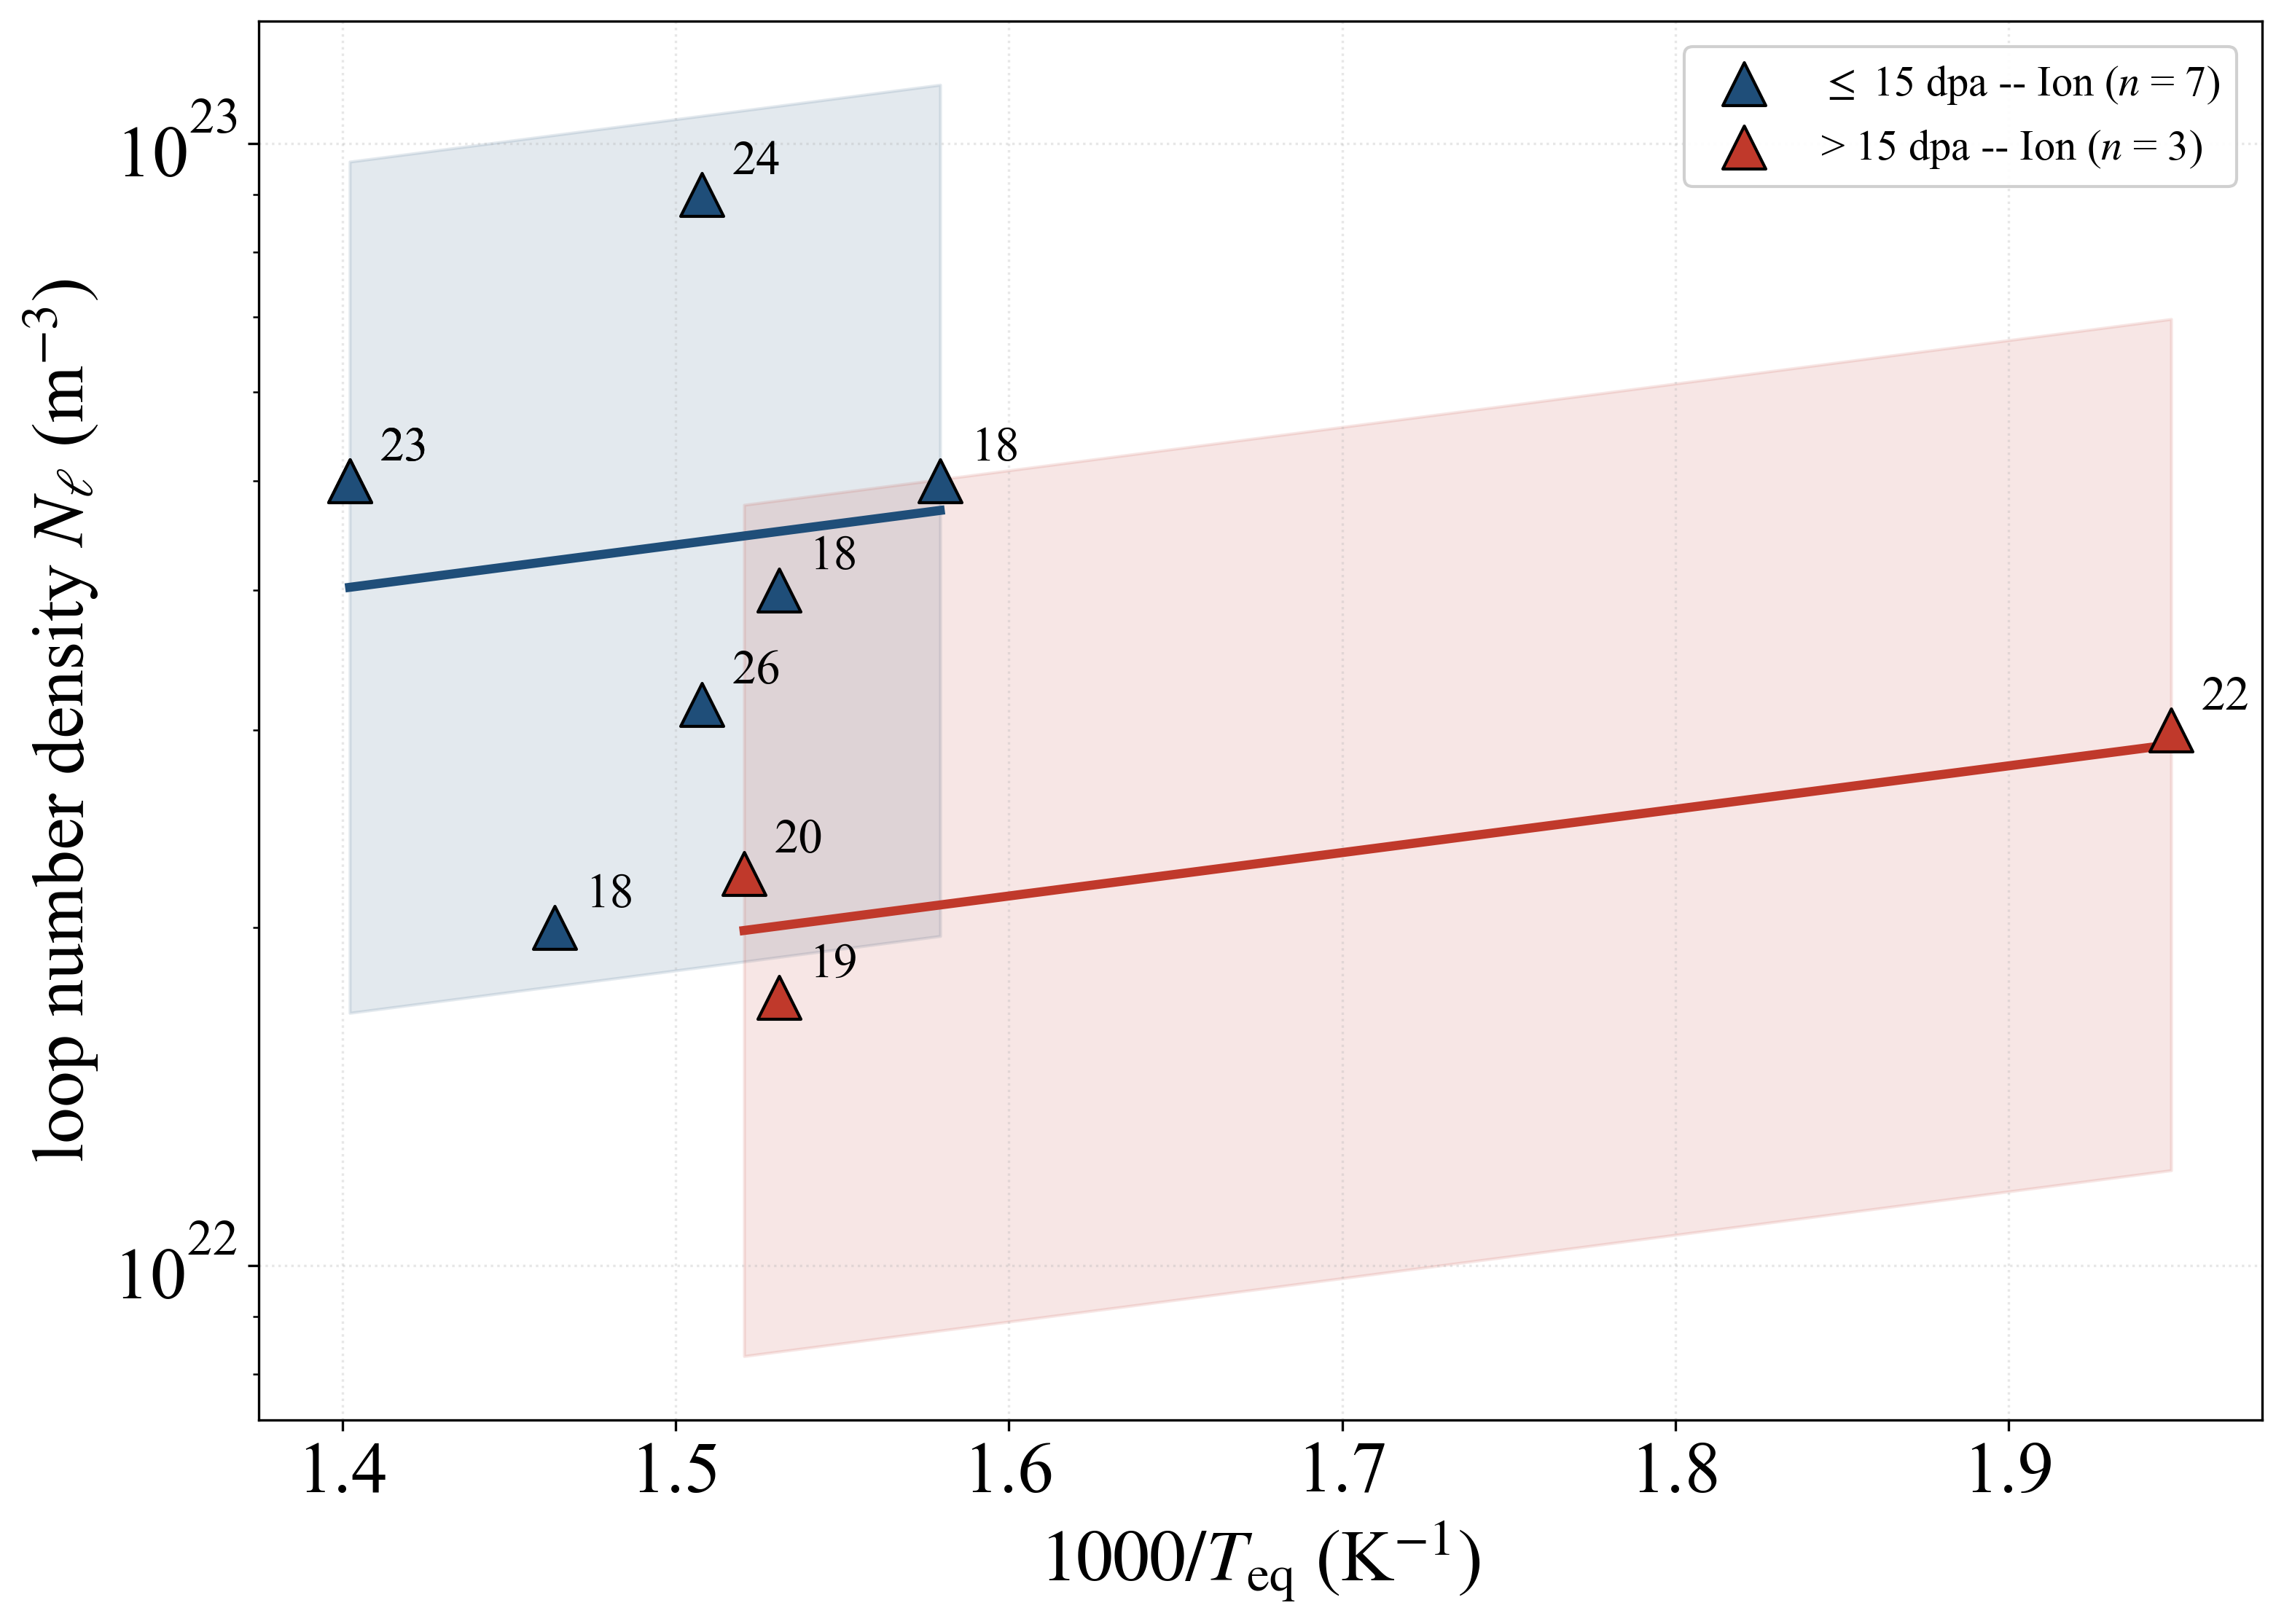
\includegraphics[width=\linewidth]{figures/experiments/ion_loop_density_invT.png}
  \caption{The data of Figure~\ref{fig:i-ld-T} on the Arrhenius axis,
  $E_{\rm eff} = -0.077 \pm 0.099$~eV. The dose offset is unchanged
  ($\times 0.45$); the thermal activation is again consistent with zero.}
  \label{fig:i-ld-invT}
\end{figure}

\subsubsection{Mean loop diameter}

The ion loop size shows the complementary behaviour: no temperature dependence at
all ($b = -8.3\times10^{-5} \pm 1.78\times10^{-3}$~K$^{-1}$, $t = -0.05$) but a
clear dose dependence, with a split at $30$~dpa giving
\begin{equation}
  c_{>30~\rm dpa} = +0.84 \pm 0.30 \quad (\times 2.3,\ t = +2.8),
  \label{eq:ils}
\end{equation}
$37\,\%$ of the variance removed at $p = 0.016$ (Figure~\ref{fig:i-ls-T}). At
$650$~K the fit gives $\bar d_{\ell} \approx 5.6$~nm below $30$~dpa and
$\approx 13$~nm above it, with $\mathrm{GSD} = 1.47$.

Taken with Eq.~\eqref{eq:ild}, the two ion loop panels describe a coarsening
population: between the low- and high-dose groups the mean diameter roughly
doubles while the number density roughly halves, so the loop line length
$\sim N_{\ell}\bar d_{\ell}$ is approximately conserved. That is the quantitative
statement a dose-resolved cluster-dynamics calculation should be asked to
reproduce, and it is considerably more discriminating than either panel alone.
The ODS flag, alloy family and Cr content are all rejected on this panel
($p \geq 0.16$).

\begin{figure}[htbp]
  \centering
  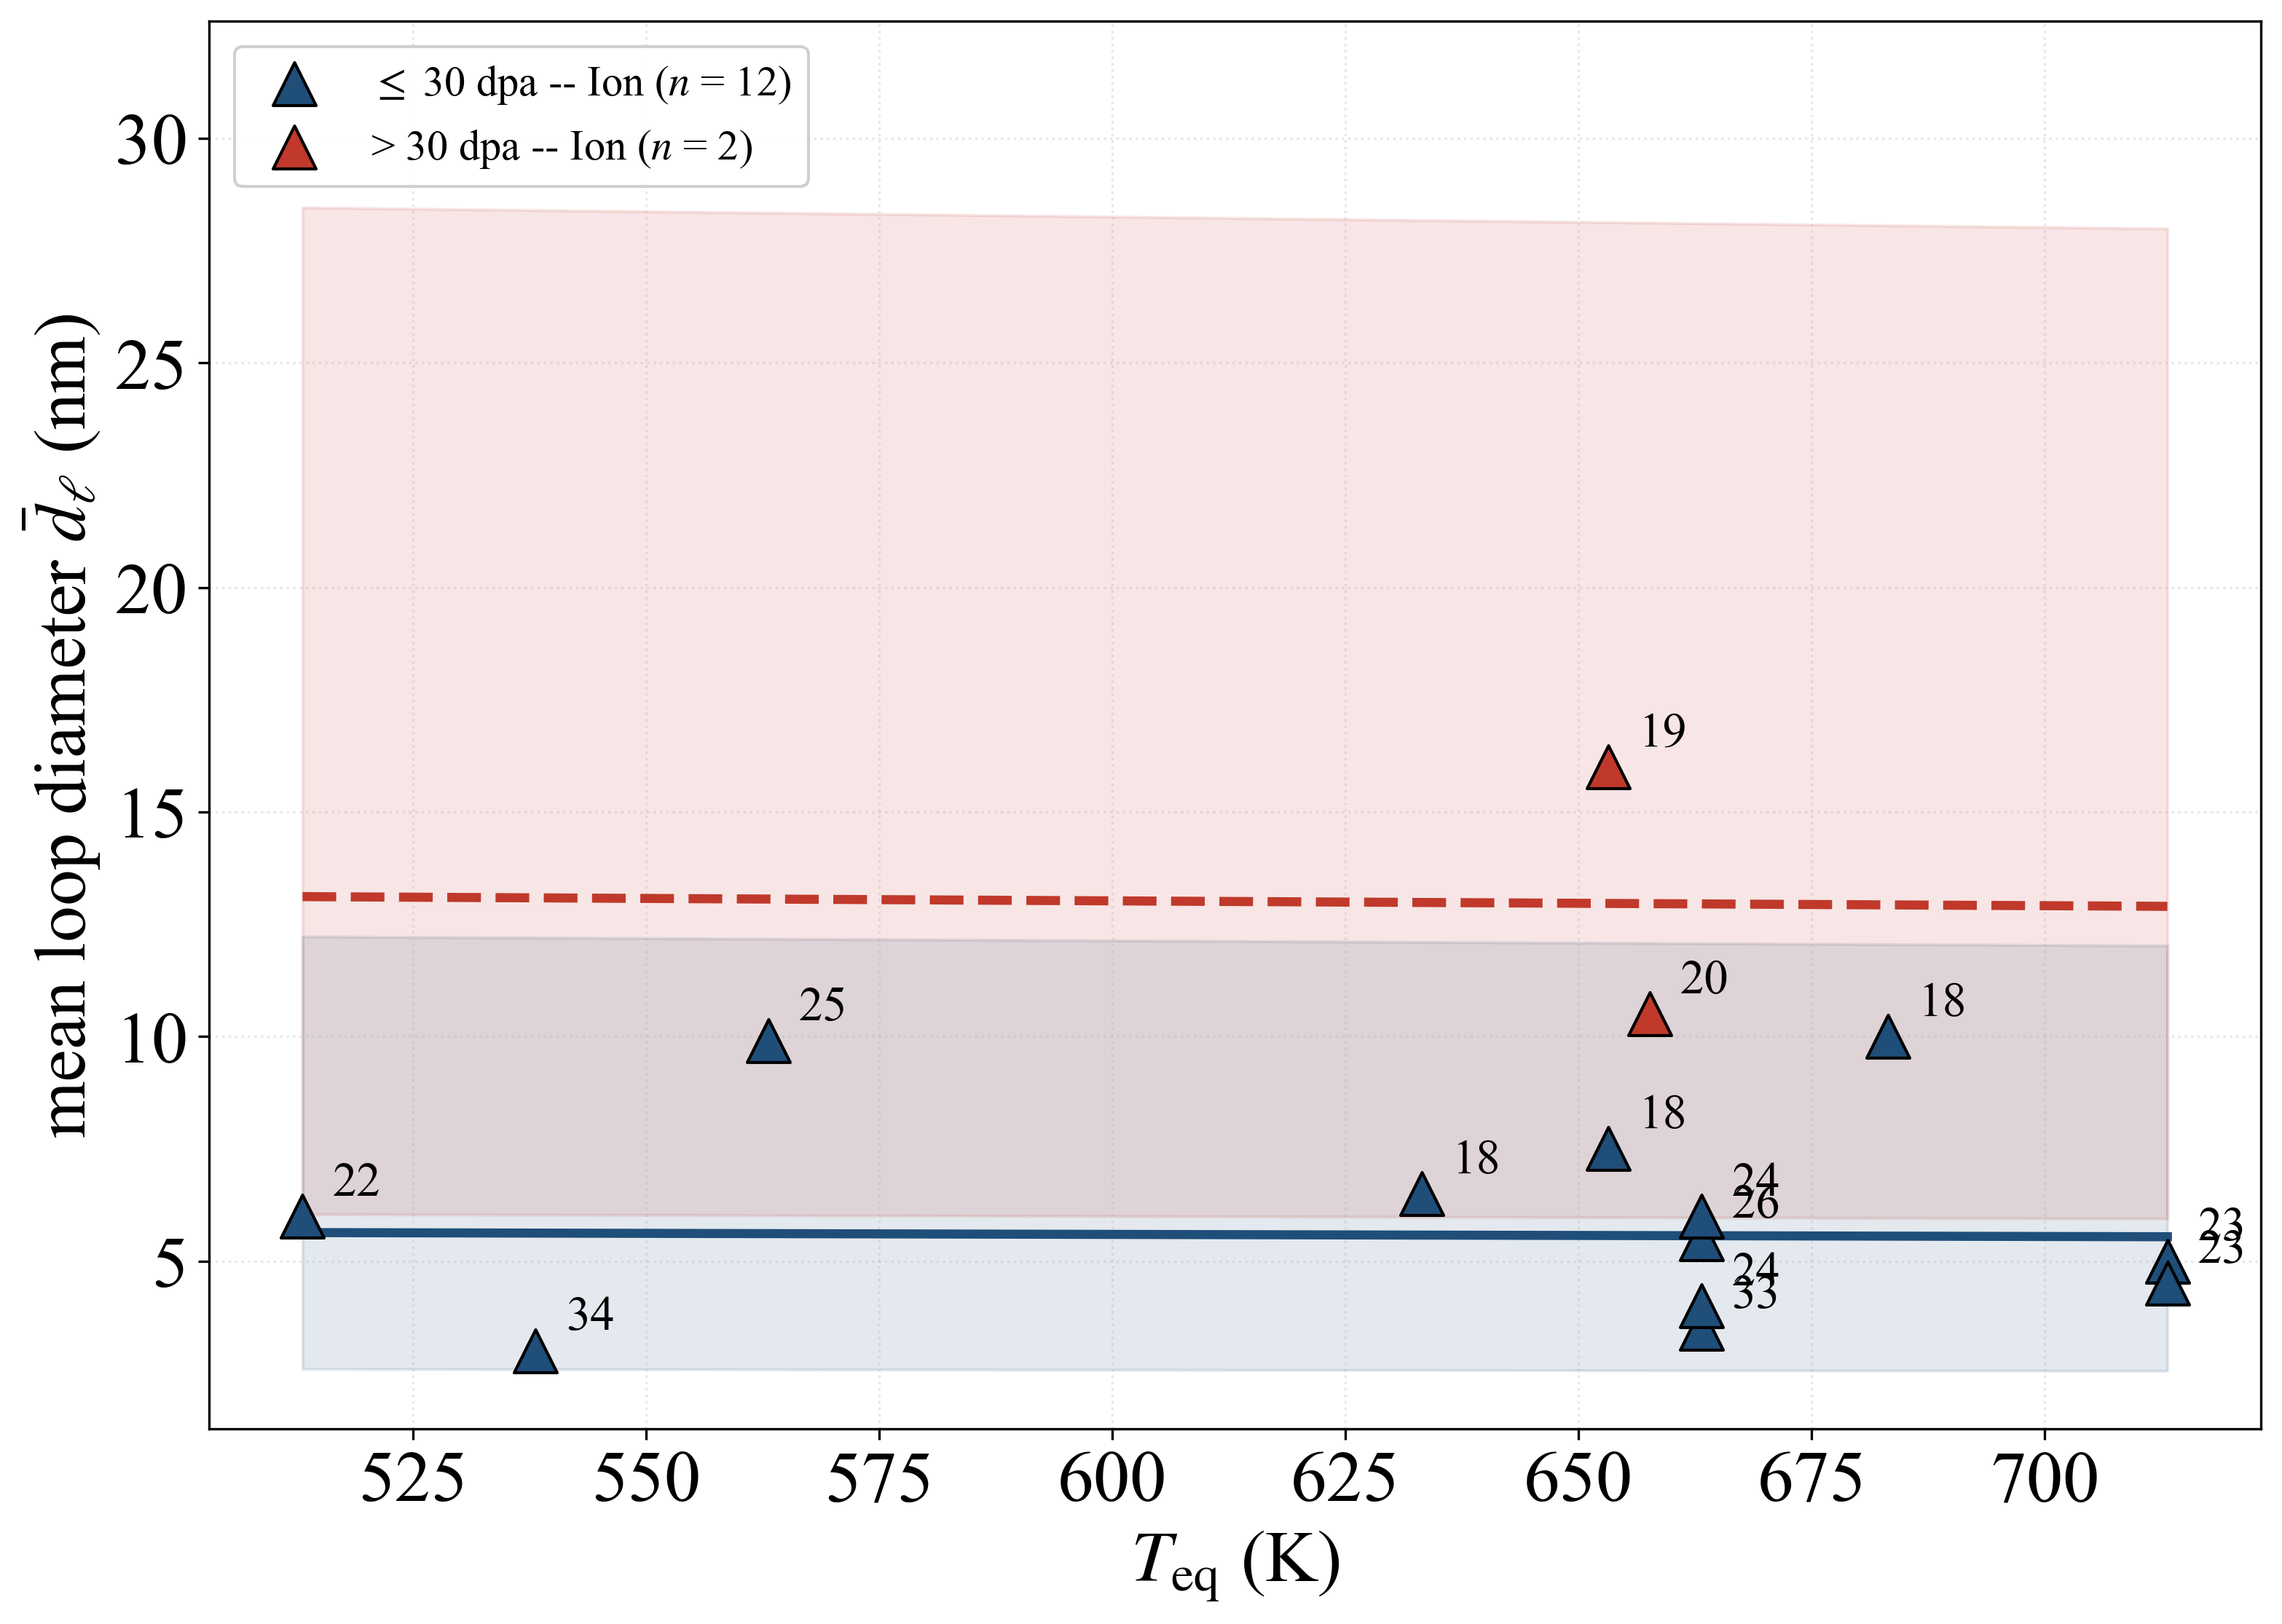
\includegraphics[width=\linewidth]{figures/experiments/ion_loop_size_T.png}
  \caption{Ion-irradiation mean loop diameter against equivalent temperature,
  grouped at $30$~dpa. The mean diameter is a factor $\approx 2.3$ larger above
  $30$~dpa while the density (Figure~\ref{fig:i-ld-T}) is about half, i.e.\ the
  population coarsens at roughly conserved loop line length. The high-dose line is
  dashed: its two rows lie $6$~K apart, so the offset is measured but the slope is
  borrowed from the low-dose group.}
  \label{fig:i-ls-T}
\end{figure}

\subsubsection{Cavity number density}

This is the largest single reduction of scatter anywhere in the database, and it
is a classification result rather than a fitting result. Separating helium
bubbles from voids (Figure~\ref{fig:i-cd-T}) removes $78\,\%$ of the variance in
$\ln N_c$ at $p = 0.0002$, taking $s^{2}$ from $3.08$ to $0.665$ and the LOO
error from $1.846$ to $0.918$. The offset is enormous,
\begin{equation}
  c_{\rm He\ bubble} = +4.49 \pm 0.74 \quad (\times 89,\ t = +6.1),
  \label{eq:icd}
\end{equation}
and the common slope is again indistinguishable from zero
($b = 1.49\times10^{-3} \pm 8.7\times10^{-3}$~K$^{-1}$; on the Arrhenius axis,
Figure~\ref{fig:i-cd-invT}, $E_{\rm eff} = +0.066 \pm 0.380$~eV). Bubbles in the
dual-beam and
He-implantation experiments sit near $3\times10^{22}$--$1\times10^{23}$~m$^{-3}$;
voids in single-beam self-ion experiments sit near
$1\times10^{20}$--$1\times10^{21}$~m$^{-3}$. Nothing else --- not the ODS flag,
not the alloy family, not $\ln(\text{dose})$ alone --- comes close.

The interpretation must be stated with its confounding. In this panel the six
He-bubble rows are at $0.2$, $0.2$, $11$, $30$, $30$ and $30$~dpa and the six
void rows are at $31.6$, $140$, $140$, $220.8$, $220.8$ and $220.8$~dpa: the
partition ``He bubble versus void'' and the partition ``dose $\leq 30$~dpa versus
$>30$~dpa'' are the \emph{same six rows}, and the two models are numerically
identical ($s^{2} = 0.665$, LOO $=0.918$ for both). This database therefore cannot
separate the effect of helium from the effect of dose on the ion cavity density.
Both readings are physically sensible --- helium stabilises a dense population of
small bubbles against thermal dissociation, and the void number density falls as
voids coarsen at high dose --- and the two-order-of-magnitude offset is almost
certainly both effects at once. A calculation reproducing the offset for the
wrong reason would be indistinguishable here; disentangling them requires
dose-matched bubble/void pairs that the database does not contain.

\begin{figure}[htbp]
  \centering
  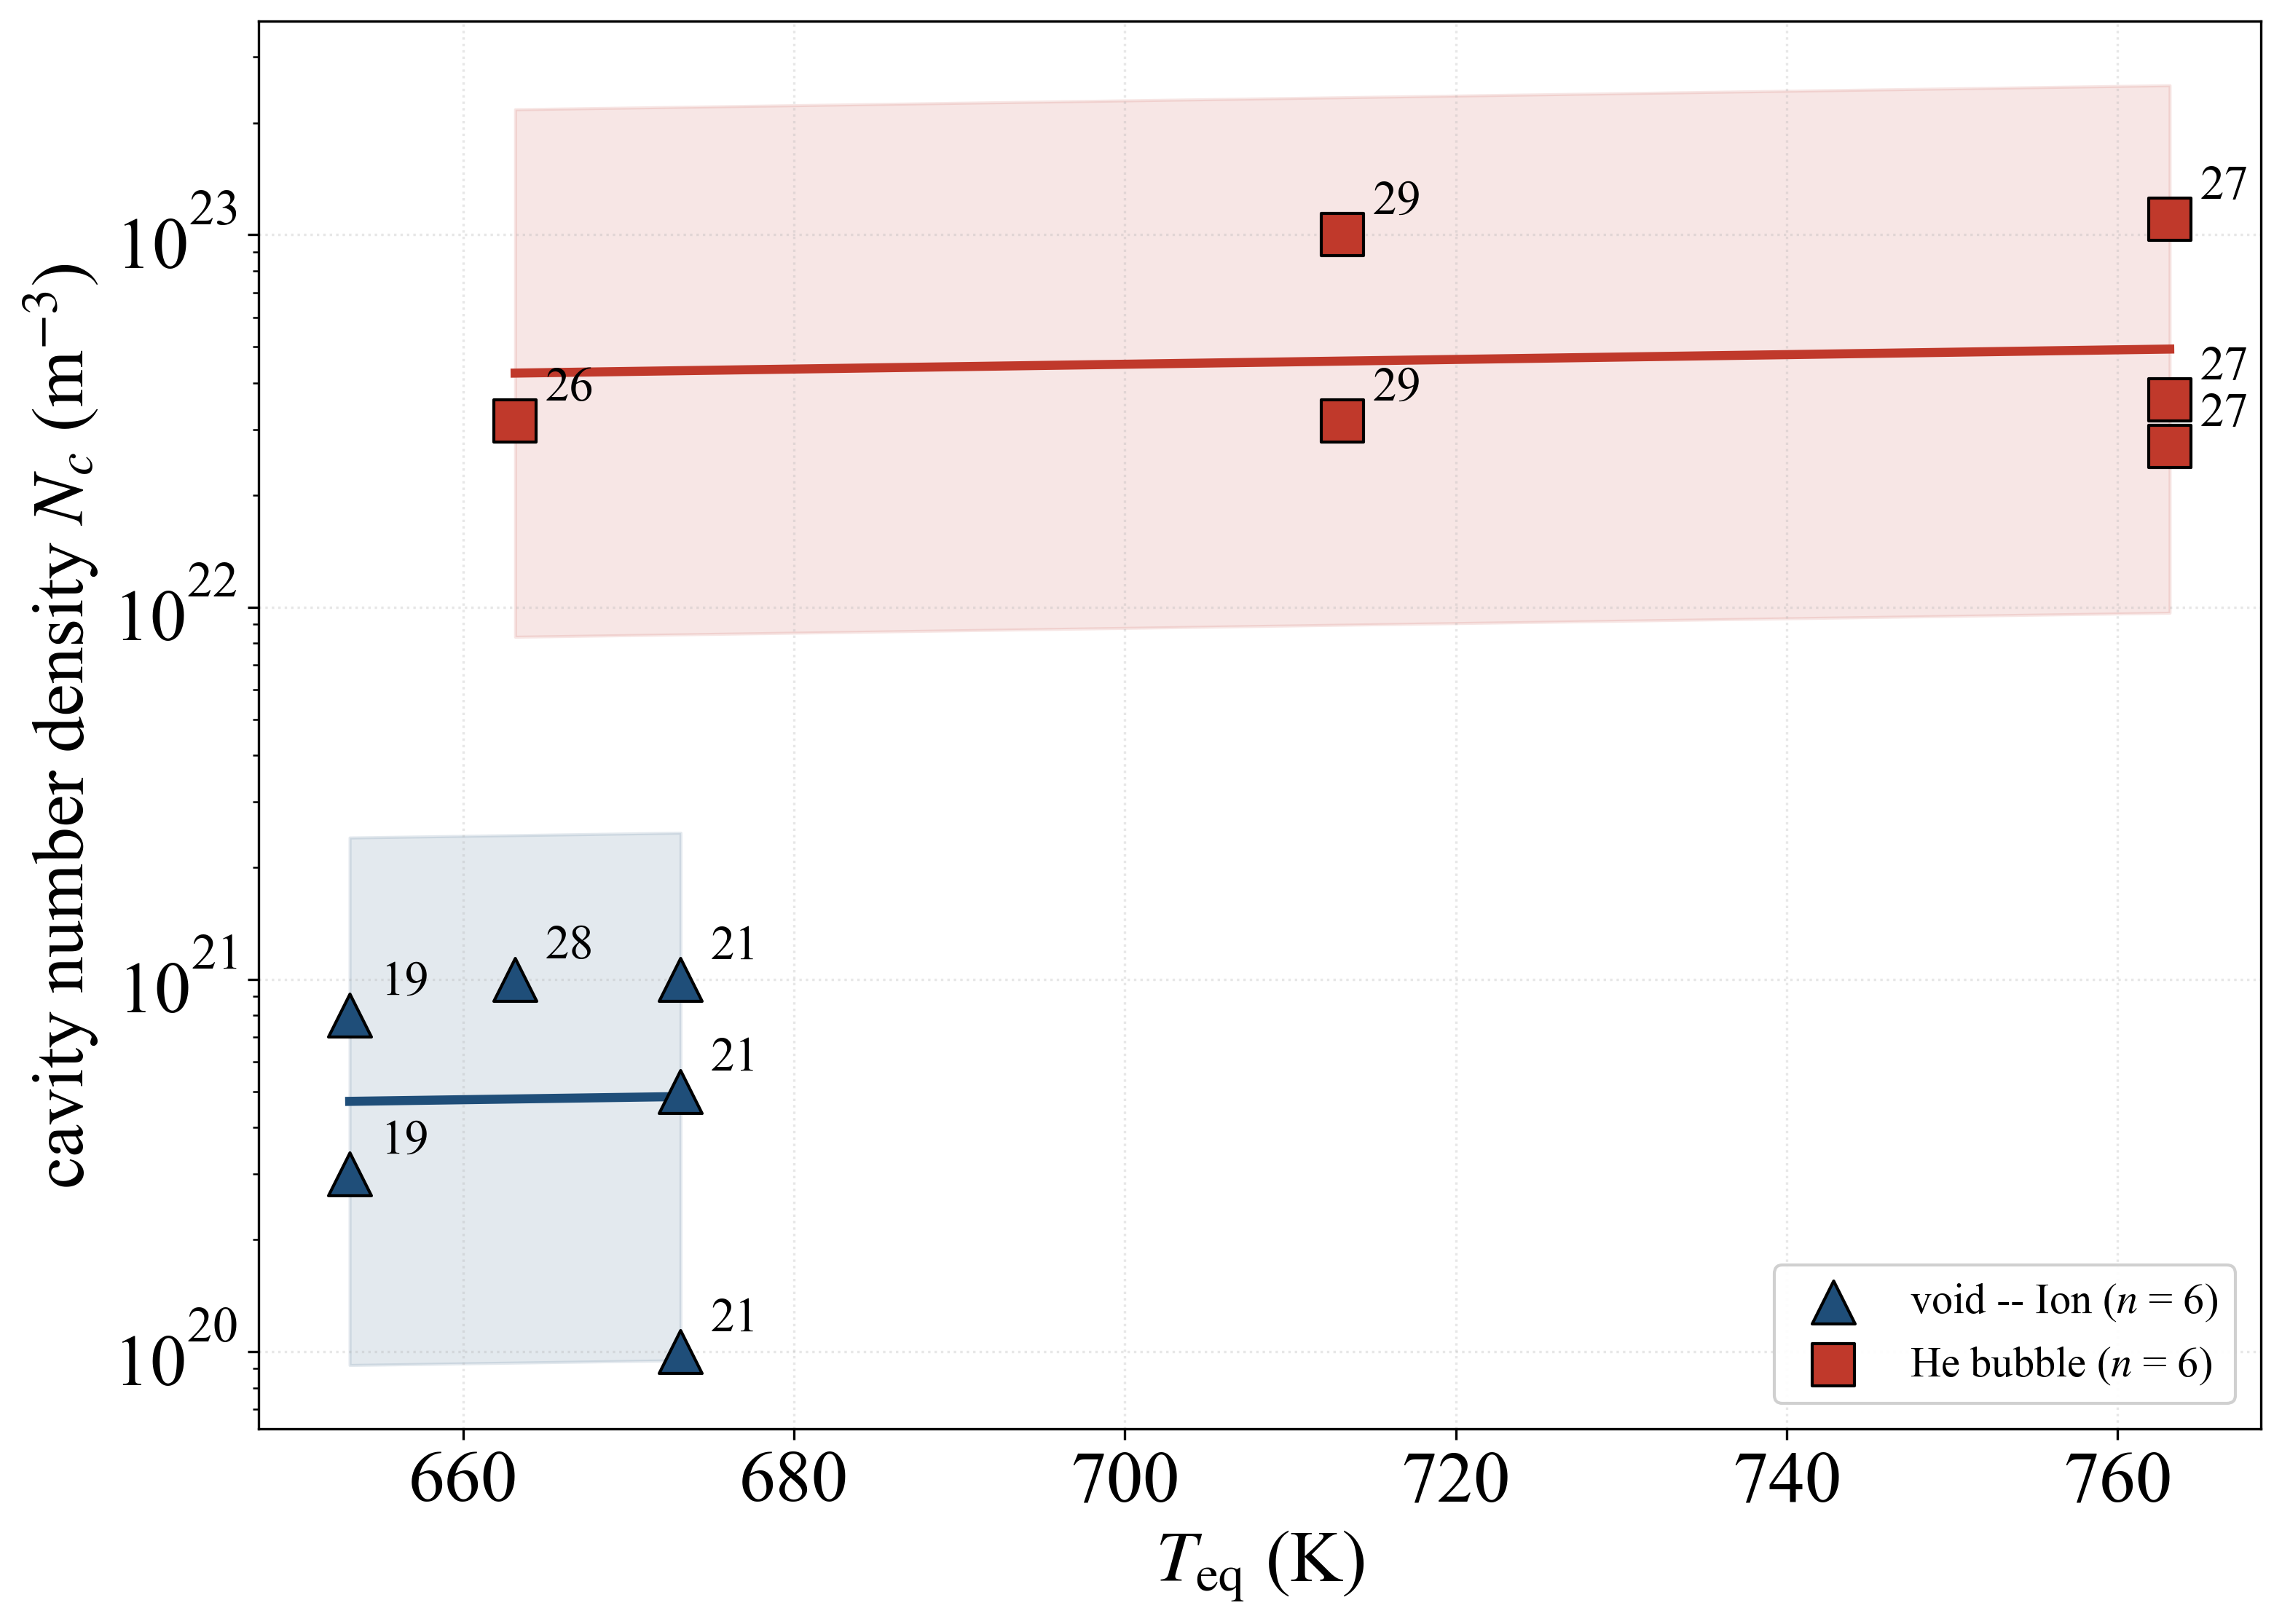
\includegraphics[width=\linewidth]{figures/experiments/ion_cavity_density_T.png}
  \caption{Ion-irradiation cavity number density against equivalent temperature,
  with helium bubbles and voids fitted as separate populations sharing a common
  temperature slope. The offset is a factor $\approx 89$. \emph{Caveat:} the six
  bubble rows are exactly the six rows at dose $\leq 30$~dpa, so this figure
  equally supports a pure dose interpretation --- the two models are numerically
  identical.}
  \label{fig:i-cd-T}
\end{figure}

\begin{figure}[htbp]
  \centering
  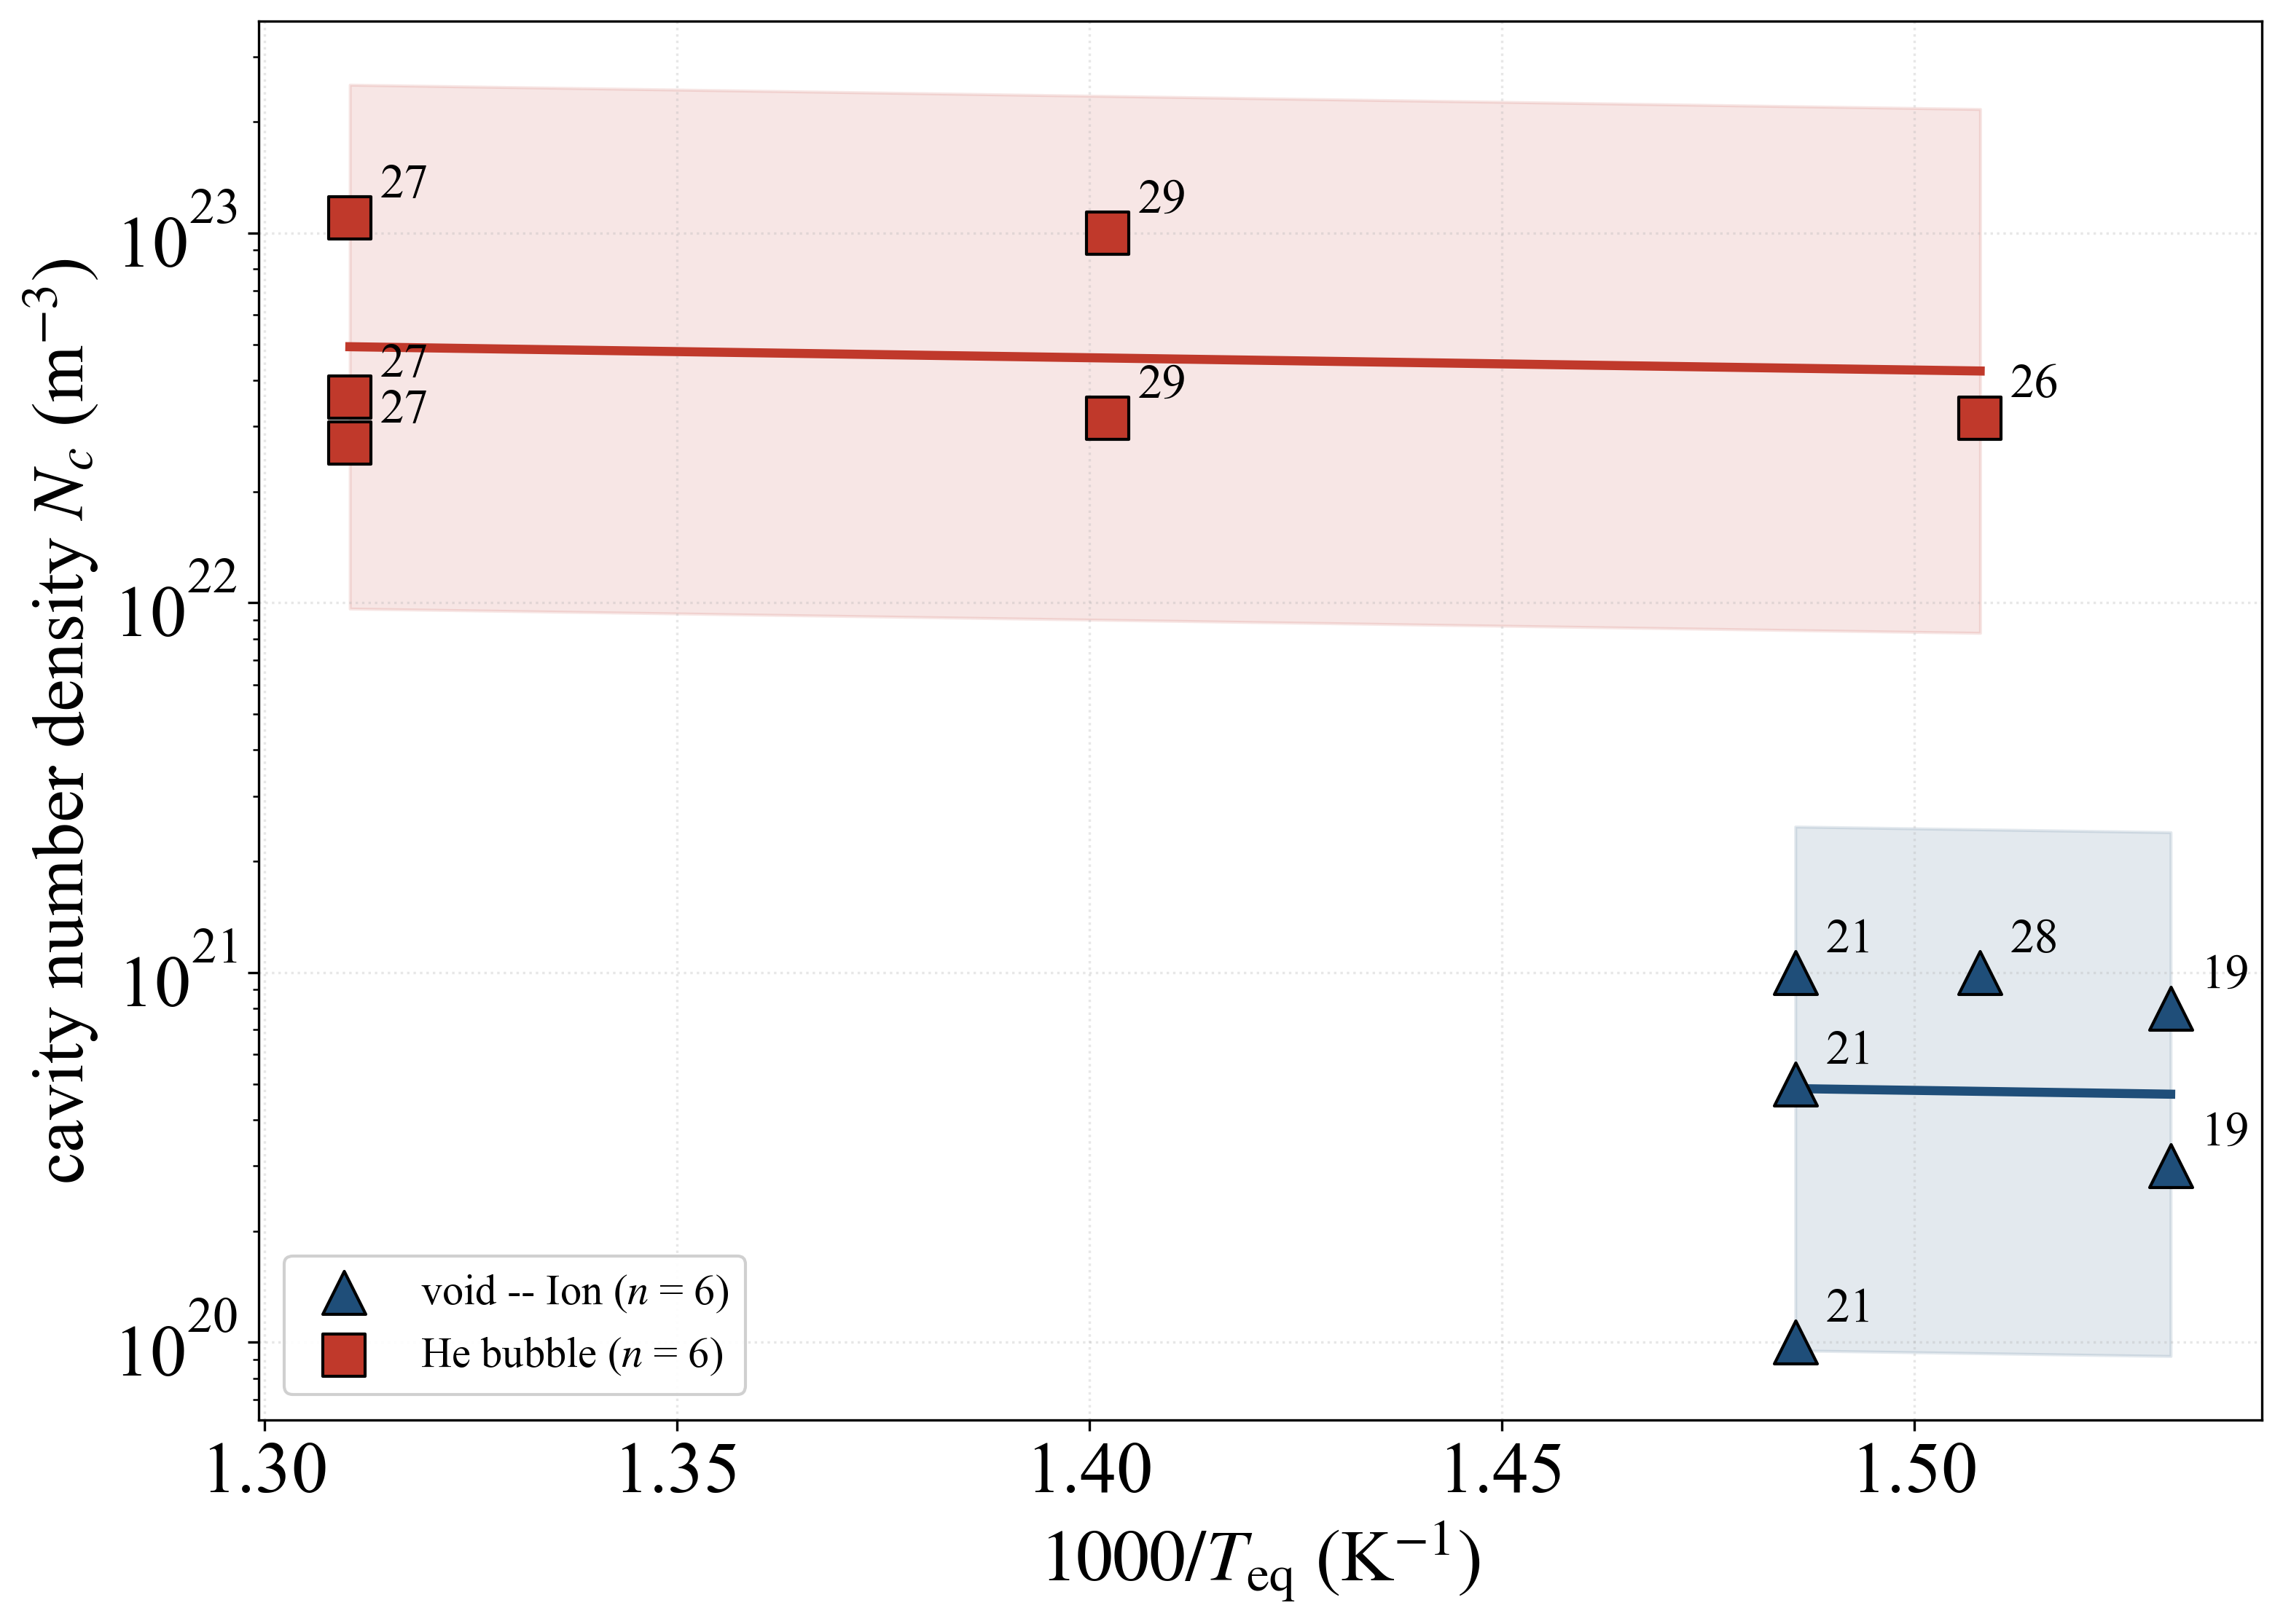
\includegraphics[width=\linewidth]{figures/experiments/ion_cavity_density_invT.png}
  \caption{The data of Figure~\ref{fig:i-cd-T} on the Arrhenius axis. The
  bubble/void offset is unchanged; the effective activation energy,
  $E_{\rm eff} = +0.066 \pm 0.380$~eV, is entirely undetermined over the
  $110$~K spanned by the ion cavity data.}
  \label{fig:i-cd-invT}
\end{figure}

\subsubsection{Mean cavity diameter}

The ion cavity size panel contains $17$ rows, one of which (source 35) reports no
dose and is plotted but not fitted. Here the dose split and the bubble/void split
are \emph{not} the same partition, and the dose split is decisively better: at
$30$~dpa it removes $67\,\%$ of the variance ($s^{2}: 0.735 \to 0.240$,
$\mathrm{LOO}\ 0.946 \to 0.528$, $p = 0.0001$) against $45\,\%$ for the
bubble/void split ($s^{2} = 0.380$, $\mathrm{LOO} = 0.669$, $p = 0.0027$). The
dose-grouped fit (Figure~\ref{fig:i-cs-T}) gives a resolved positive slope
$b = 4.01\times10^{-3} \pm 2.07\times10^{-3}$~K$^{-1}$ and
\begin{equation}
  c_{>30~\rm dpa} = +1.35 \pm 0.25 \quad (\times 3.9,\ t = +5.5),
  \label{eq:ics}
\end{equation}
i.e.\ $\bar d_c \approx 3.5$~nm below $30$~dpa and $\approx 13.5$~nm above it at
$700$~K. The bubble/void version of the same panel is shown in
Figure~\ref{fig:i-cs-bub} for comparison: bubbles are a factor $0.33$ smaller
than voids, but the split leaves twice as much residual variance as the dose
split, so on \emph{size} the dominant variable is dose.

That asymmetry is itself informative. Cavity number density is controlled by
whatever sets the nucleation site density --- helium is the natural candidate ---
whereas cavity size is controlled by accumulated vacancy flux, i.e.\ by dose.
The two ion cavity panels are therefore best used as a pair of independent
constraints rather than as one.

\begin{figure}[htbp]
  \centering
  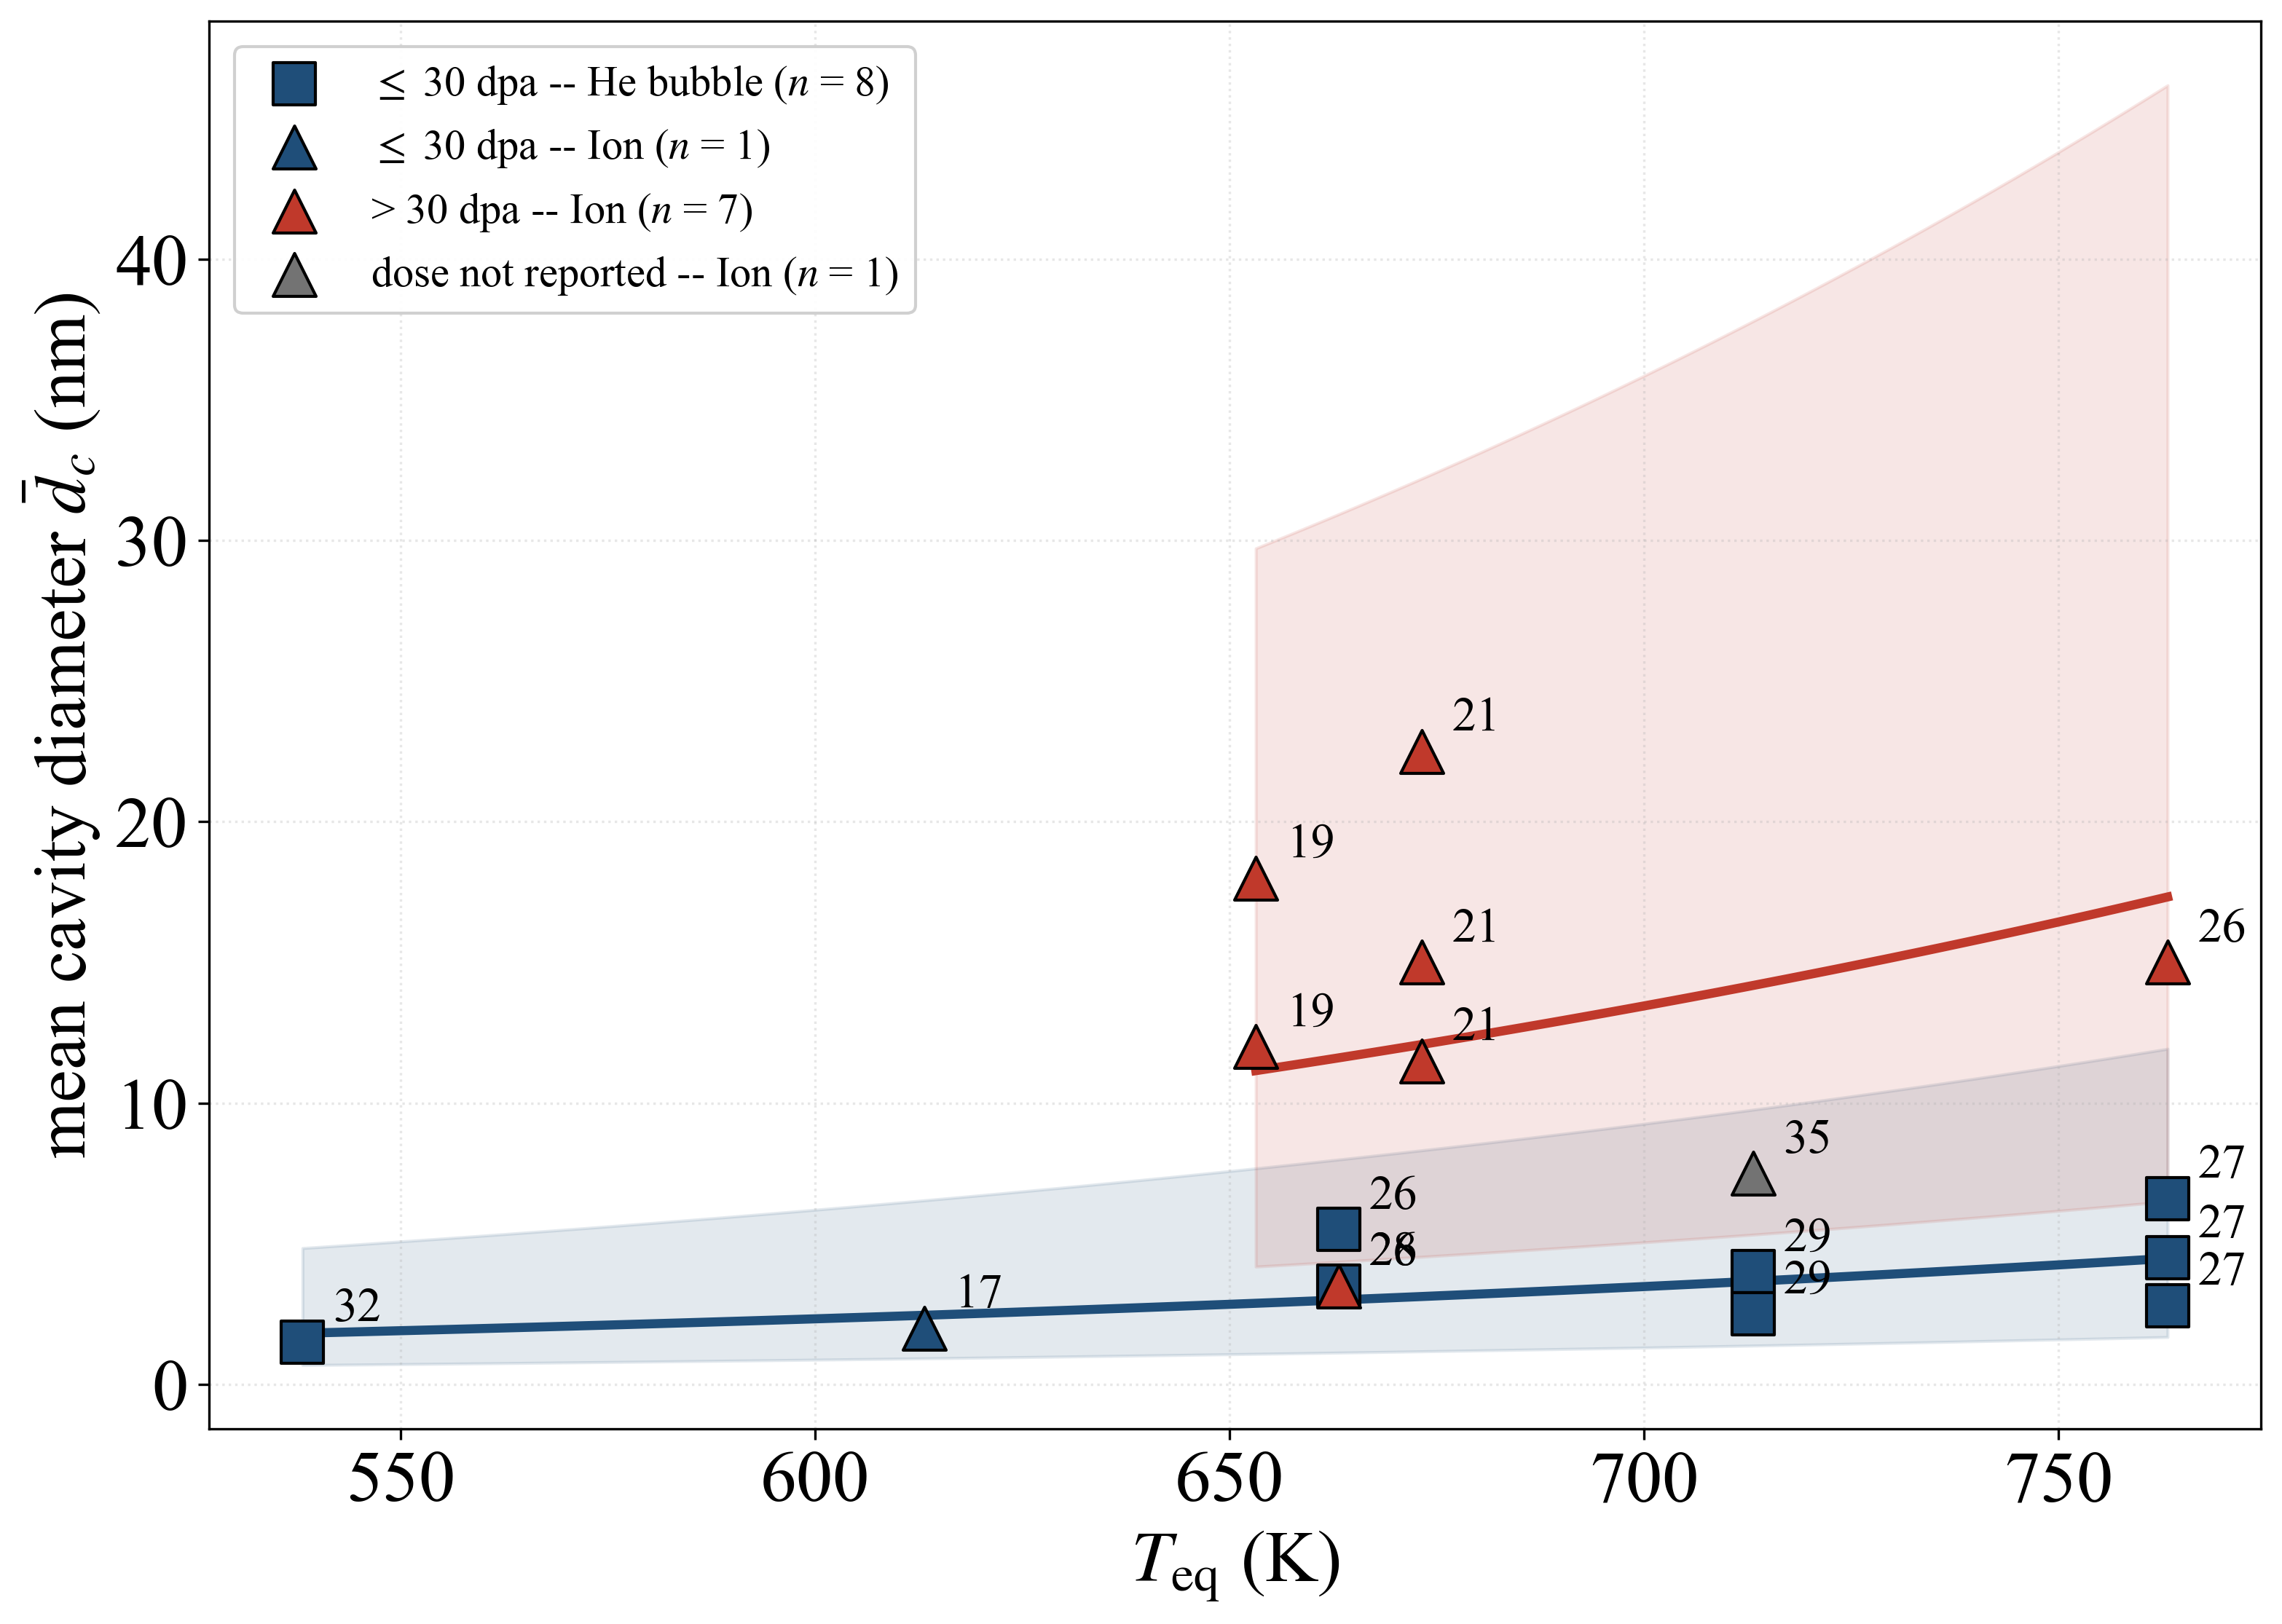
\includegraphics[width=\linewidth]{figures/experiments/ion_cavity_size_T.png}
  \caption{Ion-irradiation mean cavity diameter against equivalent temperature,
  grouped at $30$~dpa with a common slope. The grey point (source 35) reports no
  dose and is excluded from the fit. Unlike the density panel, the dose split and
  the bubble/void split are different partitions here, and the dose split is the
  better model.}
  \label{fig:i-cs-T}
\end{figure}

\begin{figure}[htbp]
  \centering
  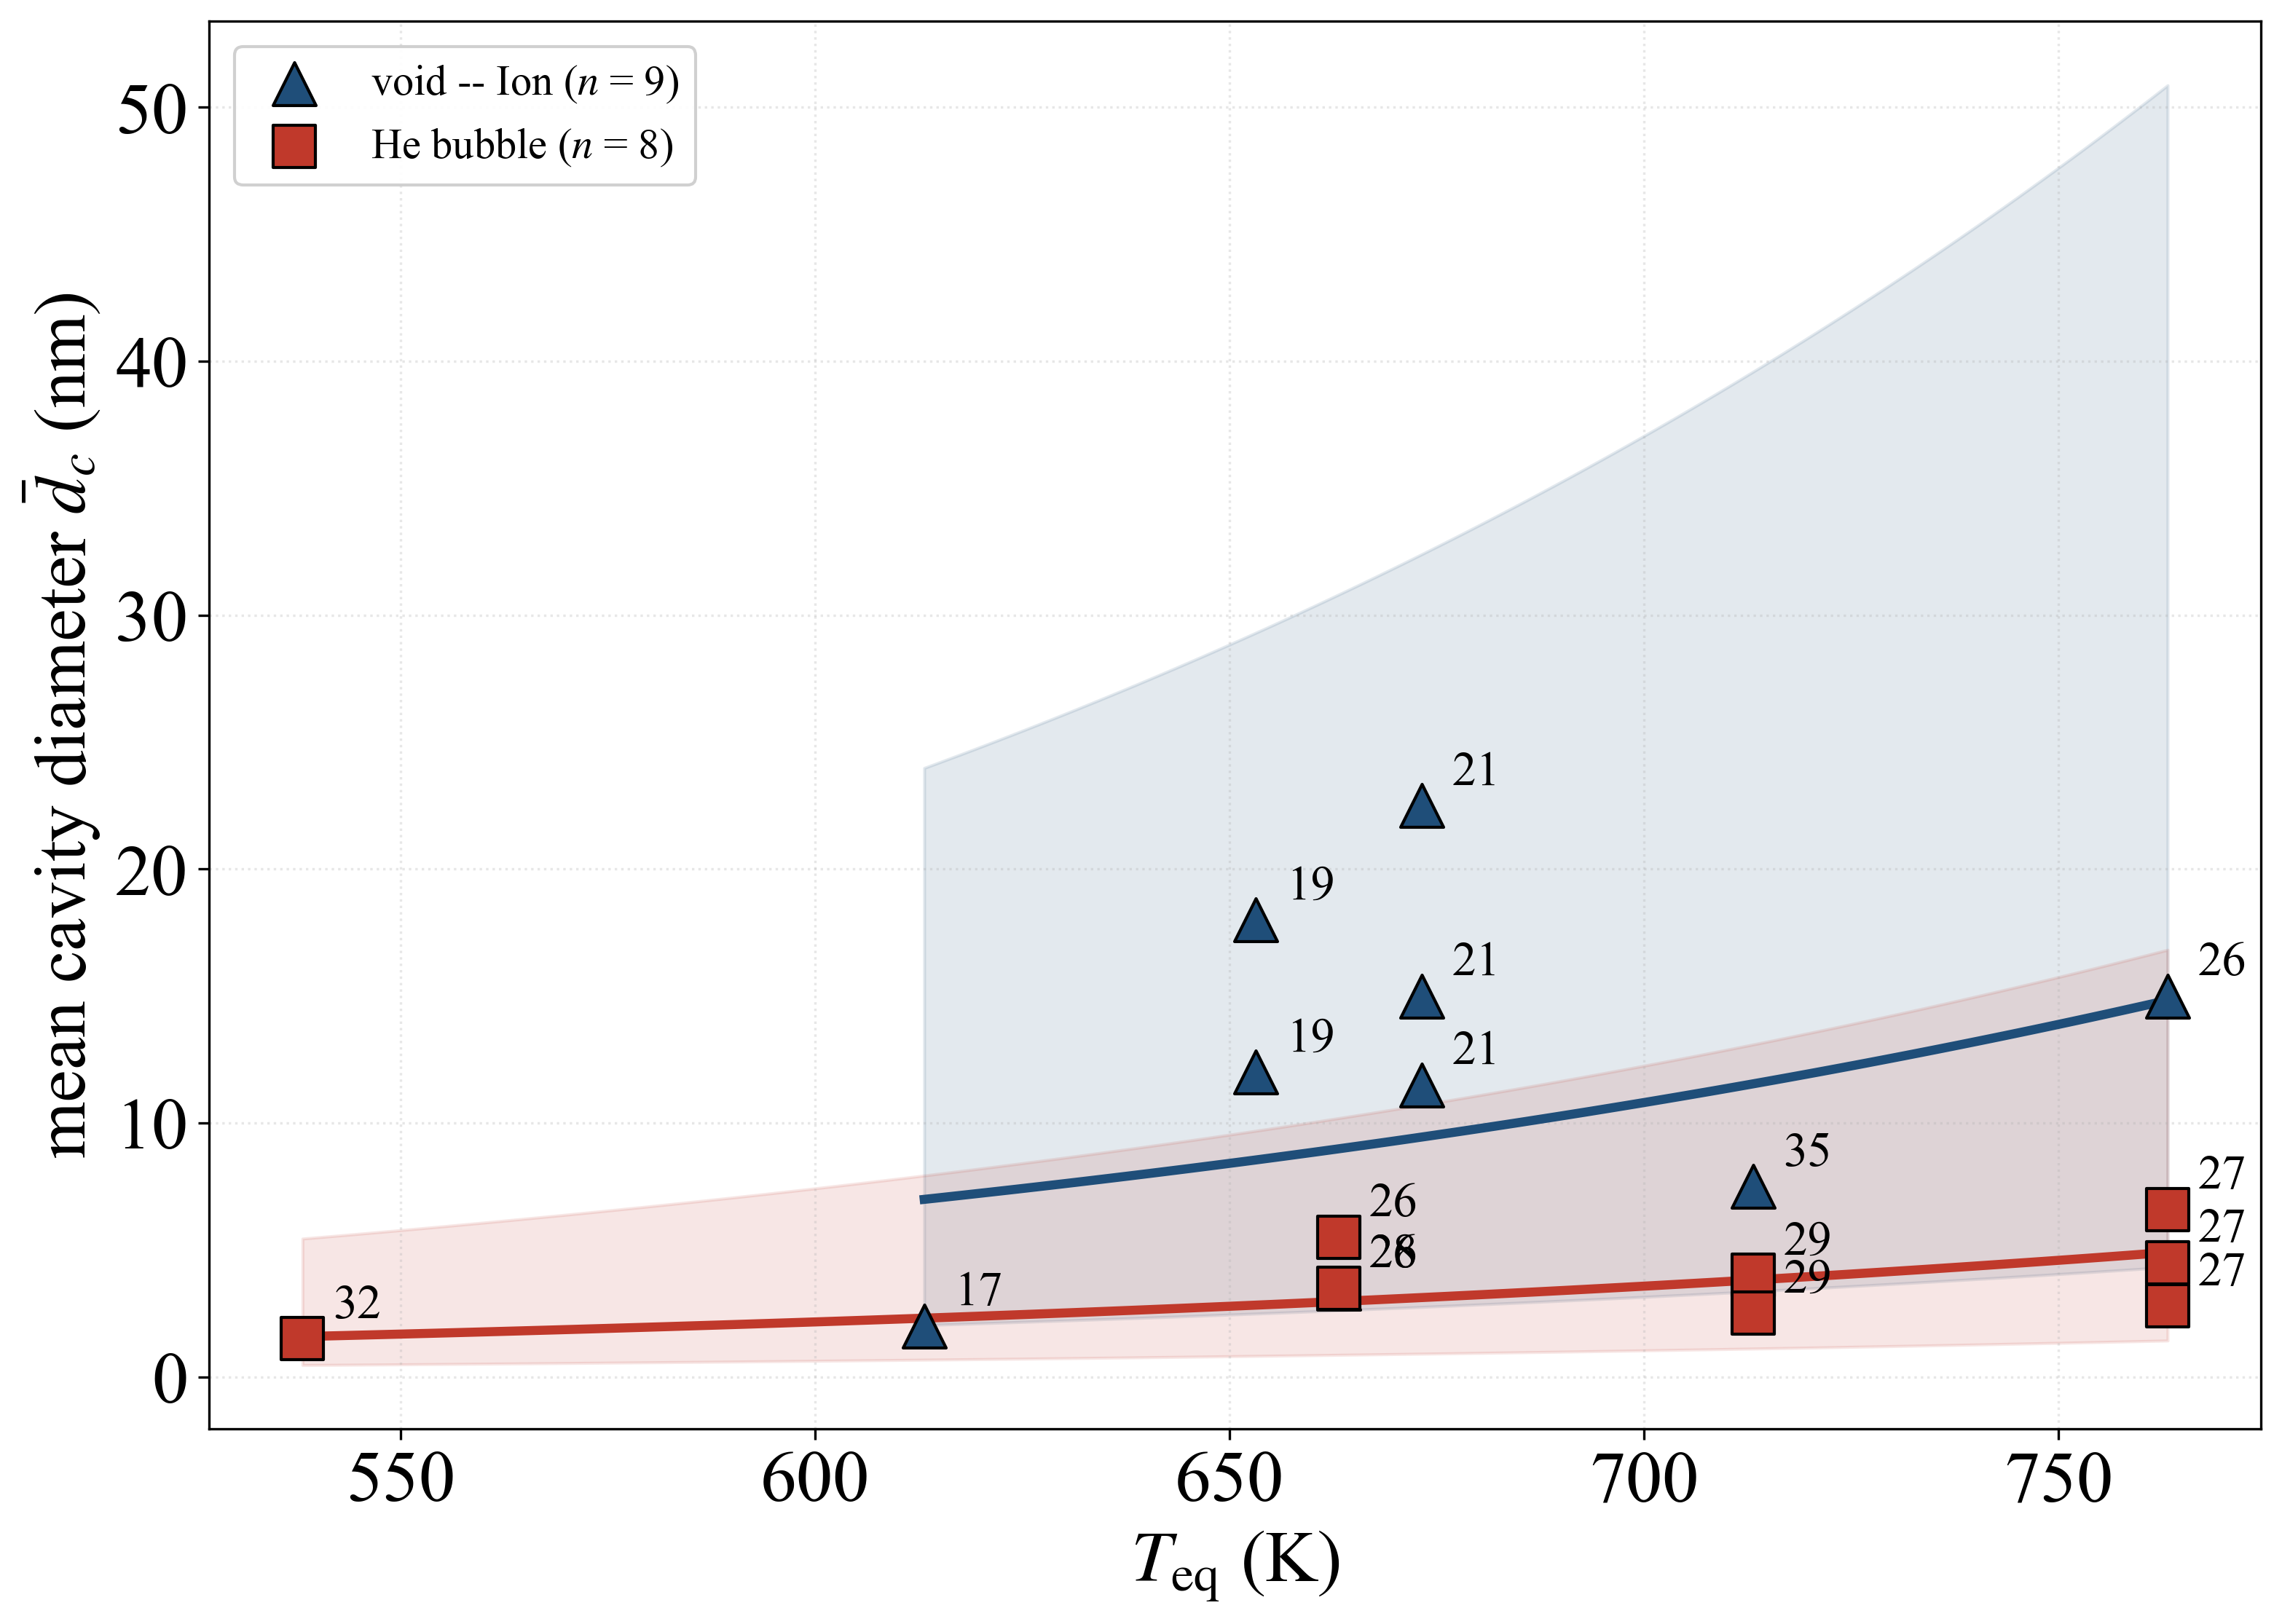
\includegraphics[width=\linewidth]{figures/experiments/ion_cavity_size_bubble_T.png}
  \caption{The panel of Figure~\ref{fig:i-cs-T} grouped instead by cavity type.
  Helium bubbles are a factor $\approx 0.33$ smaller than voids
  ($p = 0.0027$), but this split leaves $s^{2} = 0.380$ against $0.240$ for the
  dose split: on cavity size, dose is the dominant variable.}
  \label{fig:i-cs-bub}
\end{figure}

\begin{table}[htbp]
\centering\small
\caption{Model selection for all eight panels. Every candidate grouping was
fitted to each panel; $k$ is the number of regressors beyond the intercept and
the temperature term, $s^{2}$ the residual variance in $\ln y$, LOO the
leave-one-out root-mean-square prediction error in $\ln y$, and $p$ the nested
$F$-test probability against the temperature-only model. Only the
temperature-only model and the two best candidates are listed for each panel;
the complete ranking is in \texttt{figures/experiments/fit\_summary.txt}. Bold
marks the model adopted in the corresponding figure.}
\label{tab:selection}
\begin{tabular}{llrrrrr}
\toprule
Panel & Model & $k$ & $s^{2}$ & $R^{2}$ & LOO & $p$ \\
\midrule
\multicolumn{7}{l}{\emph{Neutron}}\\
Loop density ($n=19$)  & \textbf{$T$ only}          & 1 & \textbf{1.502} & 0.004 & \textbf{1.368} & --- \\
                       & $T$ + dose $>15$ dpa       & 2 & 1.326 & 0.172 & 1.318 & 0.090 \\
                       & $T$ + alloy family         & 4 & 1.764 & 0.037 & 1.509 & 0.922 \\[2pt]
Loop size ($n=19$)     & \textbf{$T$ + alloy family}& 4 & \textbf{0.178} & 0.649 & \textbf{0.569} & \textbf{0.0025} \\
                       & $T$ + ODS flag             & 2 & 0.314 & 0.291 & 0.680 & 0.035 \\
                       & $T$ only                   & 1 & 0.394 & 0.054 & 0.746 & --- \\[2pt]
Cavity density ($n=7$) & \textbf{$T$ only}          & 1 & \textbf{0.970} & 0.863 & \textbf{3.285} & --- \\
                       & $T$ + dose $>15$ dpa       & 2 & 1.063 & 0.880 & 3.481 & 0.495 \\[2pt]
Cavity size ($n=7$)    & \textbf{$T$ only}          & 1 & \textbf{0.133} & 0.545 & \textbf{0.408} & --- \\
                       & $T$ + dose $>15$ dpa$^{a}$ & 2 & 0.018 & 0.951 & 0.354 & 0.004 \\
\midrule
\multicolumn{7}{l}{\emph{Ion}}\\
Loop density ($n=10$)  & \textbf{$T$ + dose $>15$ dpa} & 2 & \textbf{0.193} & 0.422 & \textbf{0.454} & \textbf{0.067} \\
                       & $T$ + $\ln$(dose)          & 2 & 0.147 & 0.558 & 0.405 & 0.024 \\
                       & $T$ only                   & 1 & 0.282 & 0.033 & 0.545 & --- \\[2pt]
Loop size ($n=14$)     & \textbf{$T$ + dose $>30$ dpa} & 2 & \textbf{0.150} & 0.425 & \textbf{0.443} & \textbf{0.016} \\
                       & $T$ + ODS flag             & 2 & 0.217 & 0.170 & 0.508 & 0.165 \\
                       & $T$ only                   & 1 & 0.239 & 0.003 & 0.530 & --- \\[2pt]
Cavity density ($n=12$)& \textbf{$T$ + He bubble}$^{b}$ & 2 & \textbf{0.665} & 0.913 & \textbf{0.918} & \textbf{0.0002} \\
                       & $T$ + dose $>30$ dpa$^{b}$ & 2 & 0.665 & 0.913 & 0.918 & 0.0002 \\
                       & $T$ only                   & 1 & 3.079 & 0.554 & 1.846 & --- \\[2pt]
Cavity size ($n=16$)   & \textbf{$T$ + dose $>30$ dpa} & 2 & \textbf{0.240} & 0.712 & \textbf{0.528} & \textbf{0.0001} \\
                       & $T$ + He bubble            & 2 & 0.393 & 0.530 & 0.669 & 0.003 \\
                       & $T$ only                   & 1 & 0.735 & 0.051 & 0.946 & --- \\
\bottomrule
\multicolumn{7}{p{0.93\linewidth}}{\footnotesize
$^{a}$ Not adopted: with seven points and the threshold falling between rows at
$15.0$ and $15.4$~dpa, the split point was chosen by scanning and the apparent
gain is a selection effect.\quad
$^{b}$ Numerically identical models --- the six He-bubble rows are exactly the
six rows at dose $\leq 30$~dpa (Section~\ref{sec:expdb:ion}).}
\end{tabular}
\end{table}


\subsection{Loop size distributions}
\label{sec:expdb:distributions}

Six complete TEM loop-diameter histograms are available in the database, all for
neutron-irradiated EUROFER97 and EUROFER-ODS at two temperatures, and resolved by
Burgers vector where the diffraction conditions allowed it. Because a
cluster-dynamics calculation predicts the whole size distribution and not only
its mean, these are the most demanding validation targets in the database.

Each histogram is renormalised to $100\,\%$ and fitted with a two-parameter
log-normal by moment matching in $\ln d$,
\begin{equation}
  f(d) \;=\; \frac{1}{d\,\sigma\sqrt{2\pi}}
             \exp\!\left[-\frac{(\ln d - \mu)^{2}}{2\sigma^{2}}\right],
  \qquad
  \bar d = e^{\mu + \sigma^{2}/2}, \quad
  d_{\rm med} = e^{\mu}, \quad
  d_{\rm mode} = e^{\mu - \sigma^{2}},
  \label{eq:lognorm}
\end{equation}
with standard deviation $\bar d\,(e^{\sigma^{2}}-1)^{1/2}$. The fitted parameters
are given in Table~\ref{tab:dist}. Agreement is good throughout
($R^{2} = 0.88$--$0.99$) and the fitted means reproduce the mean diameters quoted
in the source papers to within $1.1\,\%$, which is a useful internal check
that the histograms and the summary rows of the database describe the same
measurements.

\subsubsection{Distributions at 300\,$^{\circ}$C}

Figure~\ref{fig:dist300} shows the three distributions measured in EUROFER97
after $15$~dpa at $300~^{\circ}$C in BOR-60, resolved by Burgers vector and
imaging area. All three are narrow and strongly peaked below $5$~nm, with
$\sigma = 0.49$--$0.54$ and means of $3.4$--$4.7$~nm. The two $\frac{1}{2}\langle
111\rangle$ populations, imaged in different areas under different diffraction
conditions ($g = \{\bar{3}10\}$ and $g = \{200\}$), give $\bar d = 4.66$ and
$4.73$~nm --- a $1.5\,\%$ difference, which is a direct measure of the
area-to-area and imaging-condition reproducibility of the technique. The
$\langle 100\rangle$ population is distinctly smaller, $\bar d = 3.41$~nm.

That the $\langle 100\rangle$ loops are the smaller population at $300~^{\circ}$C
is consistent with them forming by reaction between $\frac{1}{2}\langle
111\rangle$ loops rather than directly in cascades: the $\langle 100\rangle$
population is younger, and at this temperature the parent $\frac{1}{2}\langle
111\rangle$ loops have not yet grown large enough for the conversion to
generate a coarse product.

\begin{figure}[htbp]
  \centering
  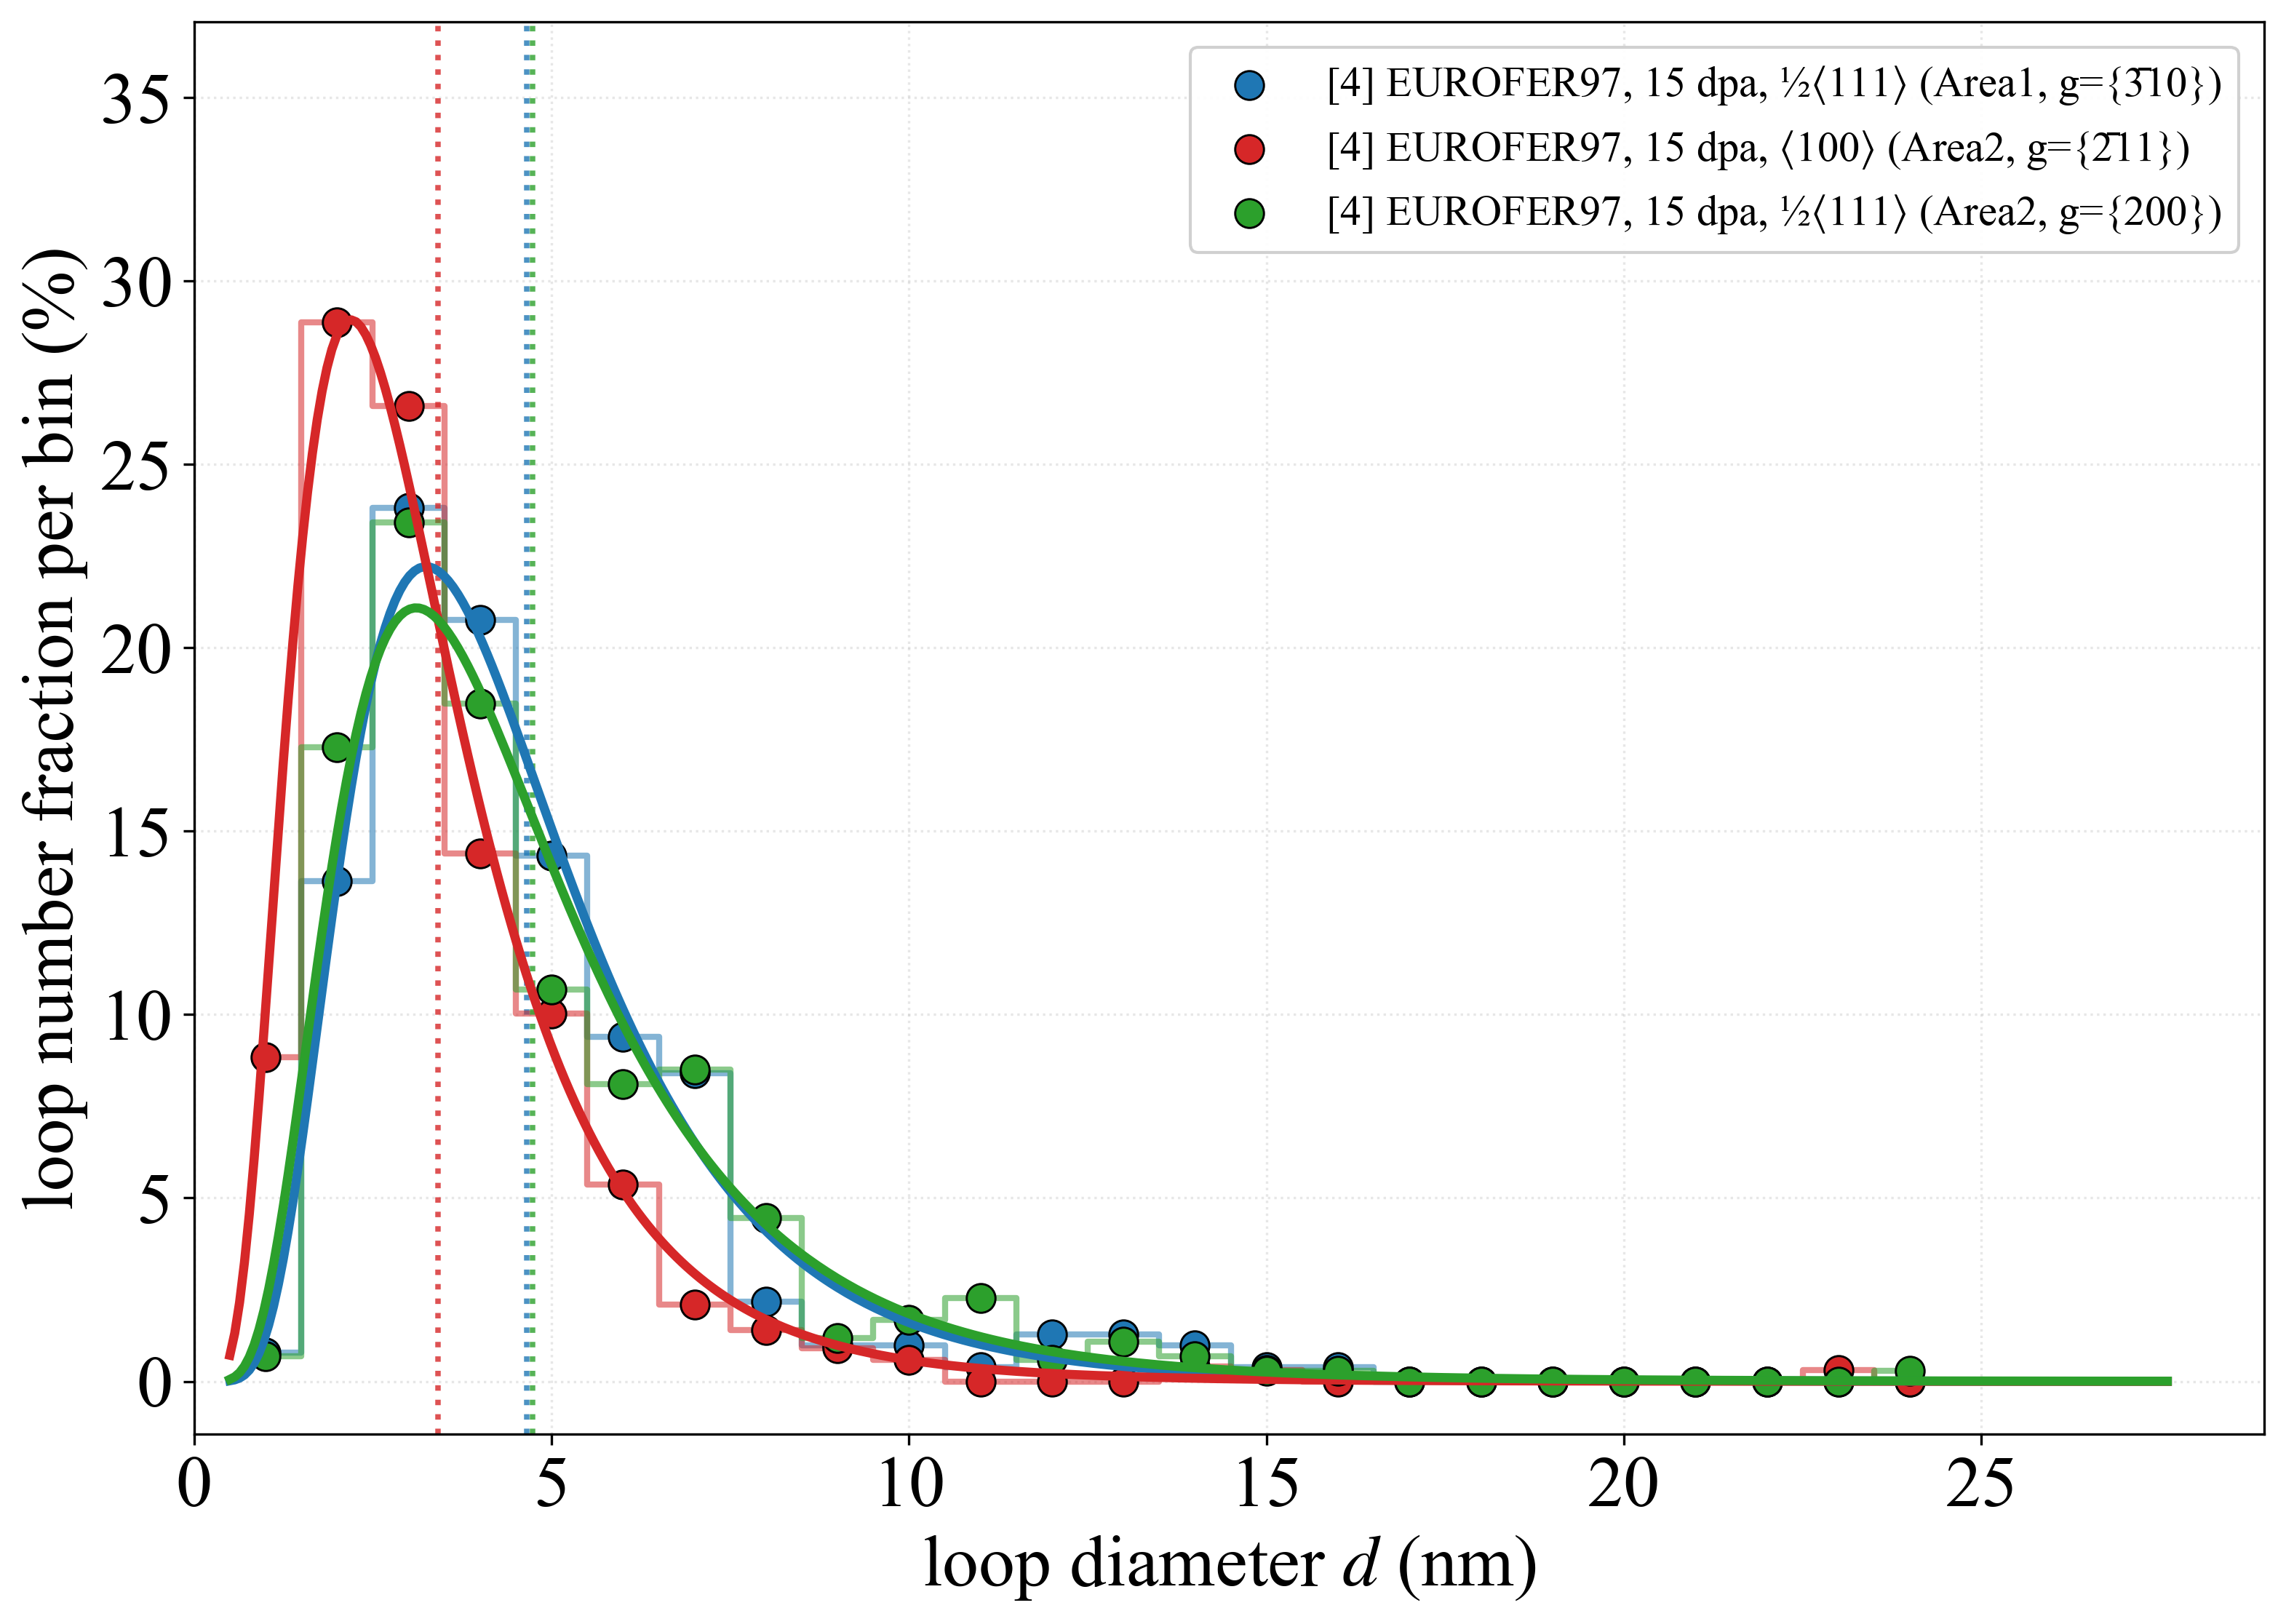
\includegraphics[width=\linewidth]{figures/experiments/loop_size_distribution_300C.png}
  \caption{Loop size distributions in EUROFER97 after neutron irradiation to
  $15$~dpa at $300~^{\circ}$C, resolved by Burgers vector and imaging area.
  Markers and thin steps are the measured per-bin fractions, thick curves the
  fitted log-normals of Eq.~\eqref{eq:lognorm}, and dotted vertical lines the
  fitted means. The two $\frac{1}{2}\langle 111\rangle$ populations, measured in
  different areas under different diffraction conditions, agree to $1.5\,\%$ in
  the mean.}
  \label{fig:dist300}
\end{figure}

\subsubsection{Distributions at 350\,$^{\circ}$C}

Figure~\ref{fig:dist350} collects the three populations available at
$350~^{\circ}$C. They are not from one experiment and must not be read as one:
the $3$~dpa distribution is EUROFER97 under $700$~keV Kr$^{2+}$ ion irradiation,
whereas the two $16.3$~dpa distributions are EUROFER-ODS after neutron
irradiation, resolved into $\langle 100\rangle$ and
$\frac{1}{2}\langle 111\rangle$ populations. The contrast is nonetheless
striking: at $16.3$~dpa the ODS material carries loops with
$\bar d = 17.2$~nm ($\langle 100\rangle$) and $26.7$~nm
($\frac{1}{2}\langle 111\rangle$), against $9.9$~nm for the $3$~dpa ion case and
$3.4$--$4.7$~nm for EUROFER97 at $300~^{\circ}$C. The
$\frac{1}{2}\langle 111\rangle$ population is now the \emph{larger} of the two,
reversing the ordering seen at $300~^{\circ}$C, and it is also the broader
($\sigma = 0.48$ against $0.39$).

\begin{figure}[htbp]
  \centering
  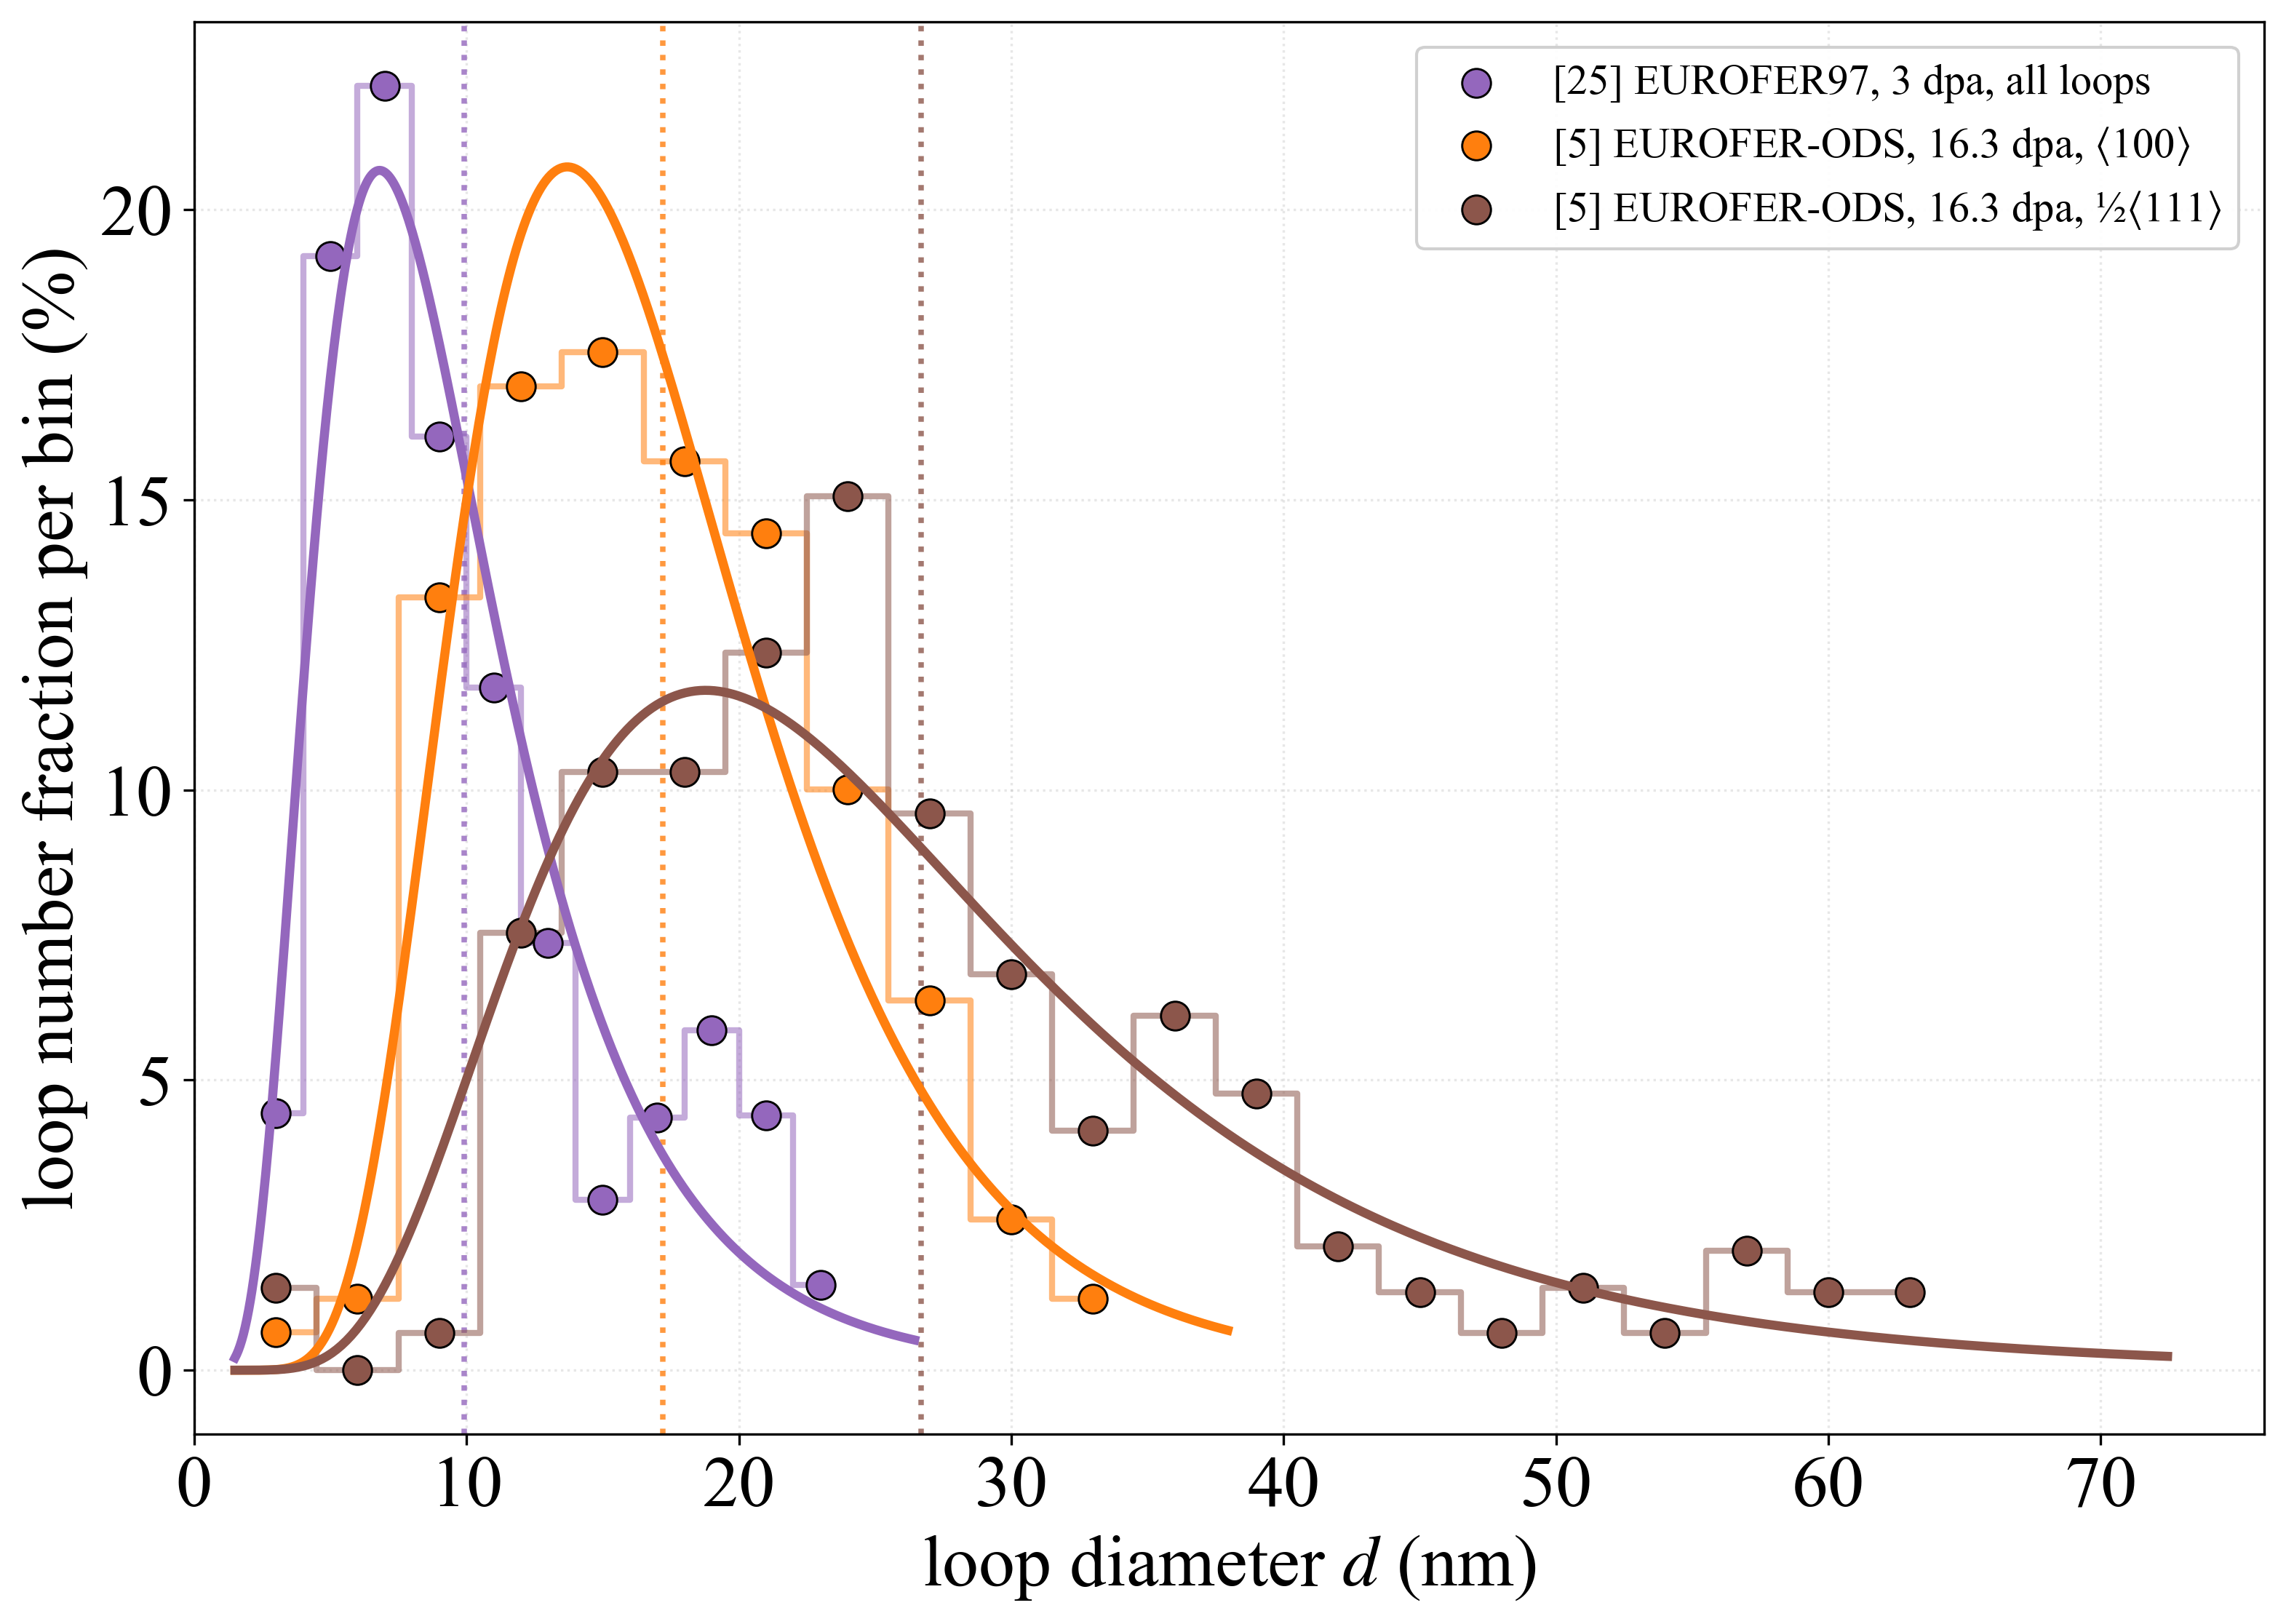
\includegraphics[width=\linewidth]{figures/experiments/loop_size_distribution_350C.png}
  \caption{Loop size distributions at $350~^{\circ}$C. The $3$~dpa distribution
  is ion-irradiated EUROFER97; the two $16.3$~dpa distributions are
  neutron-irradiated EUROFER-ODS resolved by Burgers vector. These are three
  different experiments and the comparison between them is confounded by
  irradiation type, dose and alloy simultaneously.}
  \label{fig:dist350}
\end{figure}

\subsubsection{Temperature and dose evolution}

Figure~\ref{fig:distall} places all six fitted log-normals on a common
probability-density axis. The shift is large: the mean loop diameter rises from
$3.4$--$4.7$~nm at $300~^{\circ}$C to $9.9$--$26.7$~nm at $350~^{\circ}$C, a
factor of three to six for a $50~^{\circ}$C change. The width parameter, by
contrast, is remarkably stable --- $\sigma$ lies between $0.39$ and $0.54$ across
all six distributions, two alloys, two irradiation types and a factor five in
dose. A cluster-dynamics model reproducing these data must therefore produce
distributions whose \emph{shape} in $\ln d$ is nearly invariant while their
\emph{location} moves strongly with temperature and dose; matching the mean alone
is not sufficient, and matching the width is a nearly parameter-free test.

\begin{figure}[htbp]
  \centering
  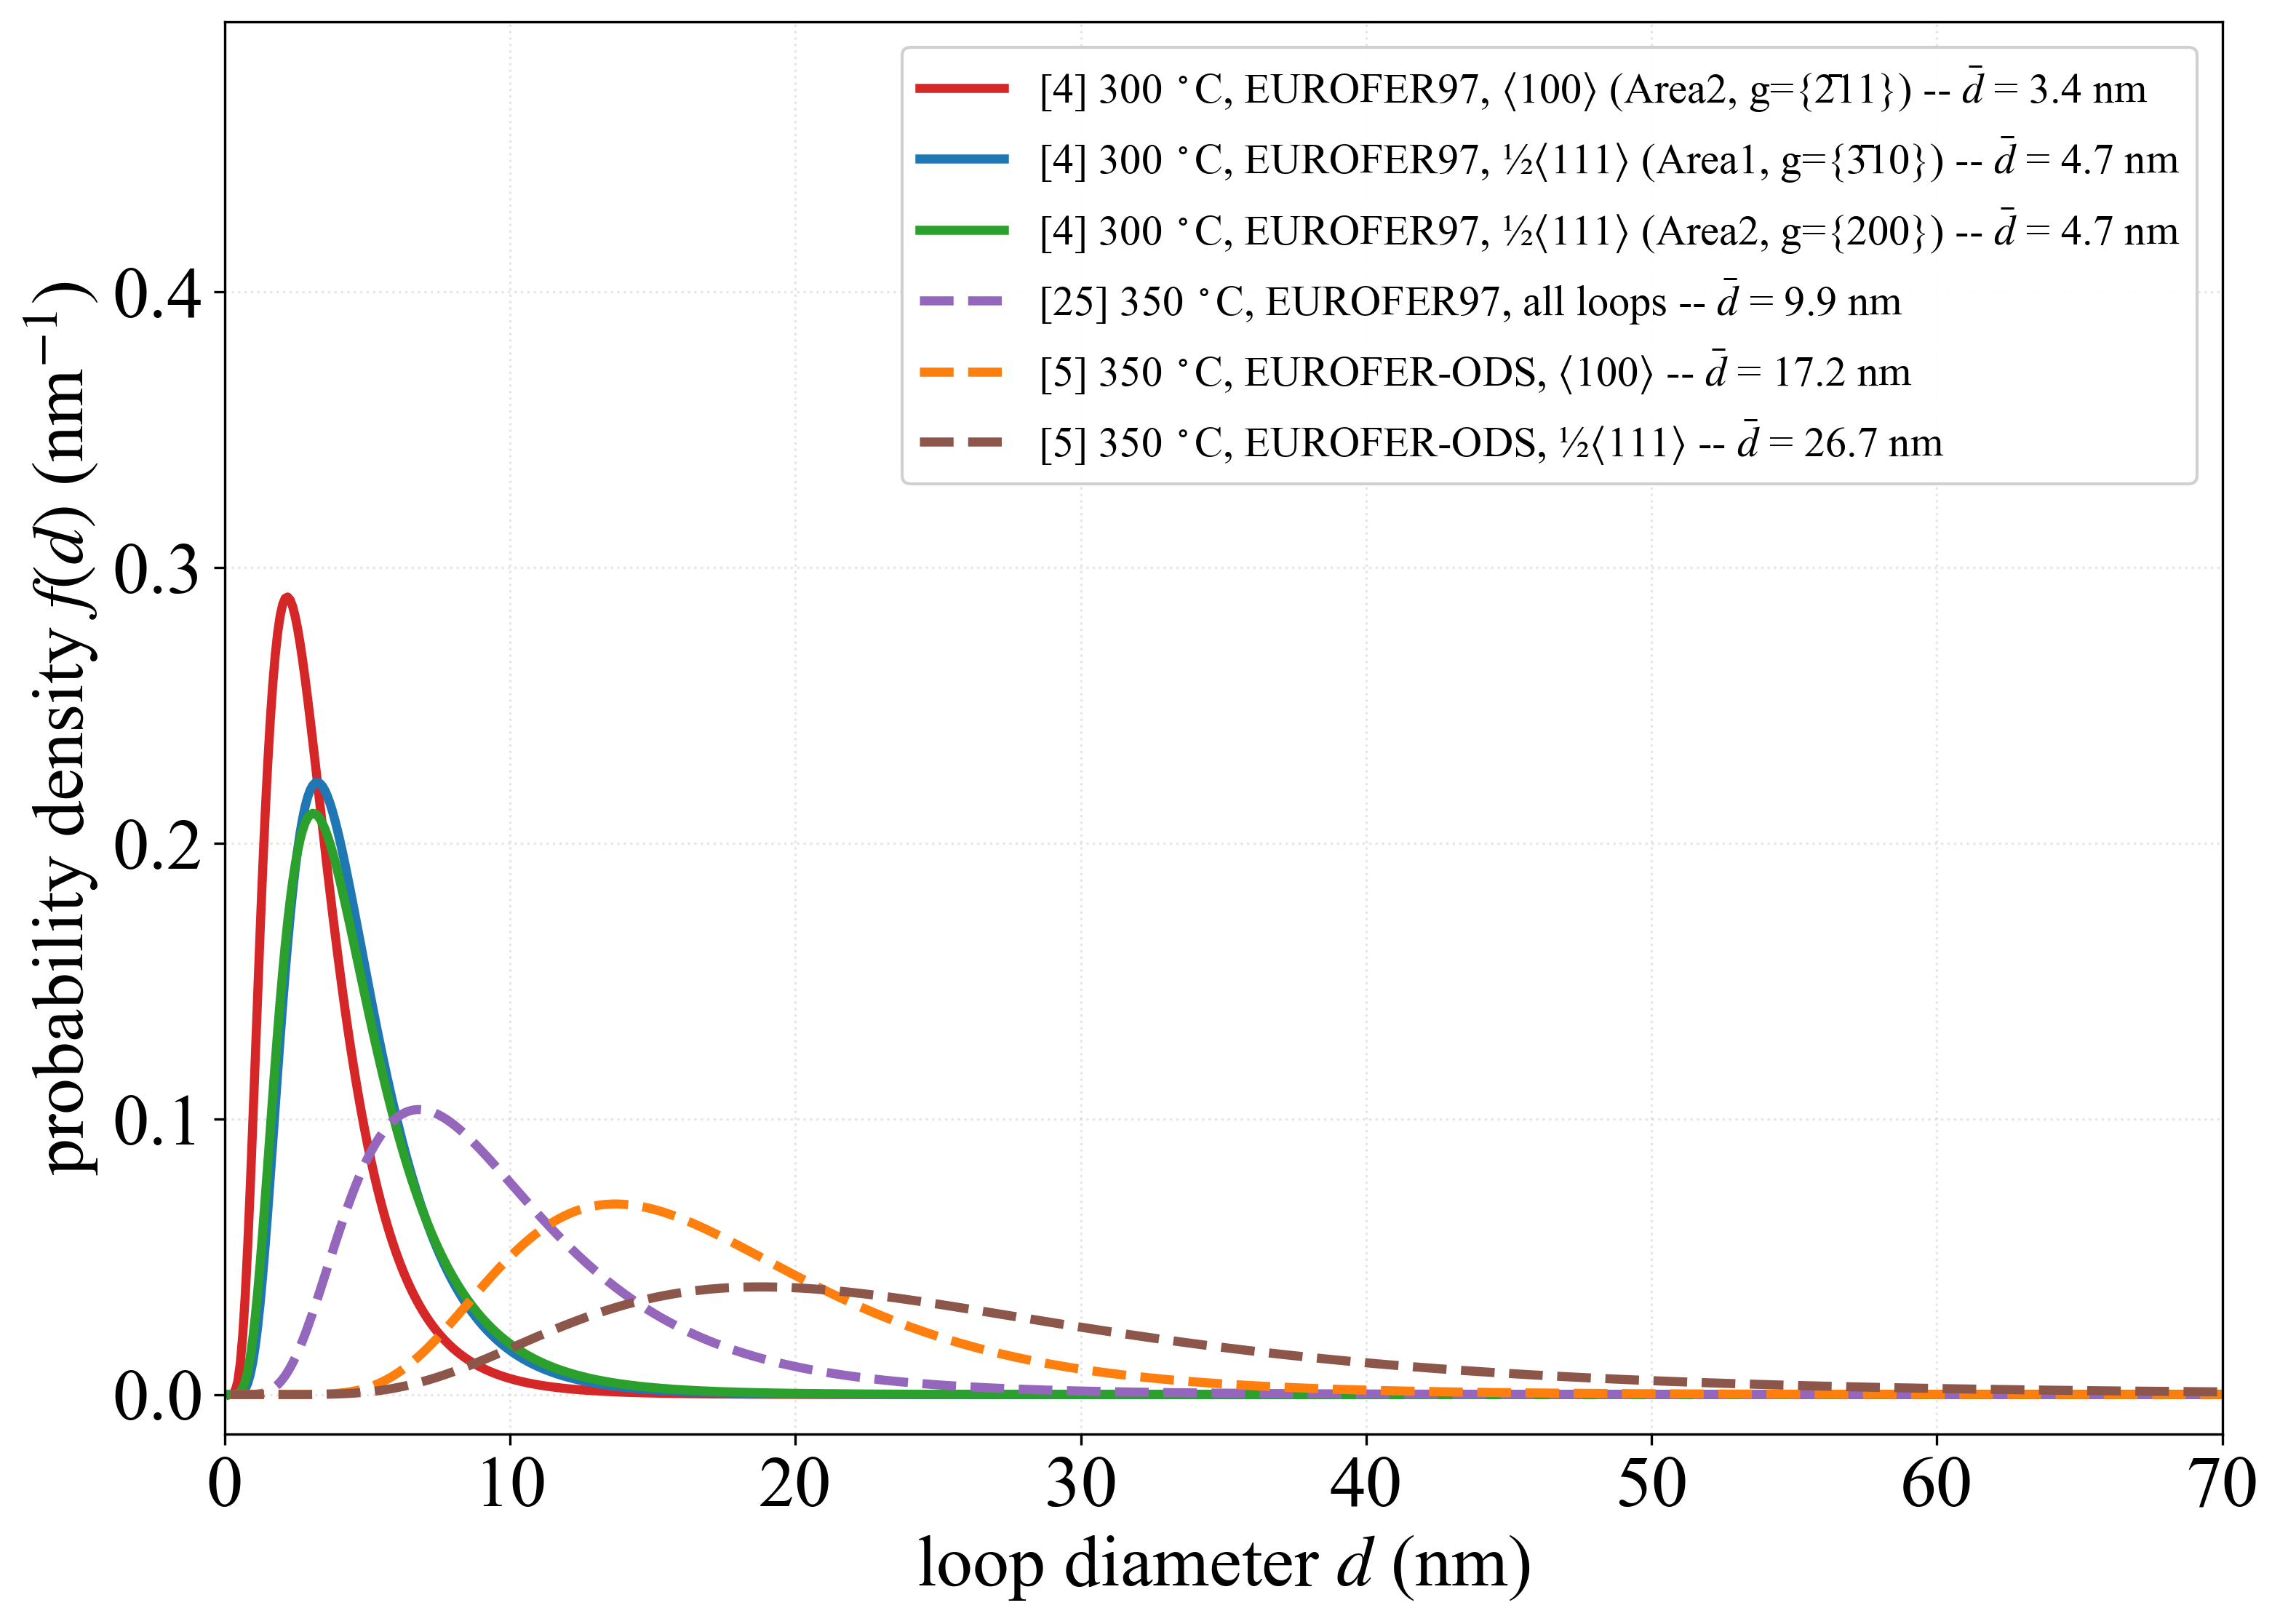
\includegraphics[width=\linewidth]{figures/experiments/loop_size_distribution_all.png}
  \caption{All six fitted log-normal loop size distributions on a common
  probability-density axis, each normalised to unit area; solid for
  $300~^{\circ}$C and dashed for $350~^{\circ}$C. The location moves by a factor
  three to six between the two temperatures while the log-normal width parameter
  stays within $\sigma = 0.39$--$0.54$ throughout.}
  \label{fig:distall}
\end{figure}

\begin{table}[htbp]
\centering\small
\caption{Log-normal parameters fitted to every measured loop size distribution
by moment matching in $\ln d$, Eq.~\eqref{eq:lognorm}. ``Source'' is the paper
number of Table~\ref{tab:refs}; SD is the standard deviation of the fitted
log-normal. All diameters in nm.}
\label{tab:dist}
\begin{tabular}{llrlrrrrrrr}
\toprule
Material & Irr. & $T$ ($^{\circ}$C) & Population & Dose & $\mu$ & $\sigma$ &
$\bar d$ & $d_{\rm med}$ & $d_{\rm mode}$ & $R^{2}$ \\
\midrule
EUROFER97   & n & 300 & $\frac{1}{2}\langle 111\rangle$, area 1 & 15.0 & 1.418 & 0.491 & 4.66  & 4.13  & 3.24  & 0.985 \\
EUROFER97   & n & 300 & $\langle 100\rangle$, area 2            & 15.0 & 1.080 & 0.543 & 3.41  & 2.94  & 2.19  & 0.993 \\
EUROFER97   & n & 300 & $\frac{1}{2}\langle 111\rangle$, area 2 & 15.0 & 1.414 & 0.529 & 4.73  & 4.11  & 3.11  & 0.966 \\
EUROFER97   & i & 350 & all loops                               &  3.0 & 2.168 & 0.500 & 9.91  & 8.74  & 6.81  & 0.915 \\
EUROFER-ODS & n & 350 & $\langle 100\rangle$                    & 16.3 & 2.770 & 0.390 & 17.22 & 15.95 & 13.70 & 0.919 \\
EUROFER-ODS & n & 350 & $\frac{1}{2}\langle 111\rangle$         & 16.3 & 3.167 & 0.484 & 26.68 & 23.73 & 18.78 & 0.877 \\
\bottomrule
\end{tabular}
\end{table}


\subsection{Loop character: the $\langle 100\rangle$ fraction}
\label{sec:expdb:fraction}

Sections~\ref{sec:expdb:neutron} and~\ref{sec:expdb:ion} treat the loop population
as one species. It is not: irradiated bcc iron and its alloys carry two distinct
interstitial loop families, $\frac{1}{2}\langle 111\rangle$ loops, which are glissile
and formed directly in cascades, and $\langle 100\rangle$ loops, which are sessile and
--- on the prevailing reaction picture --- formed largely by interaction between
$\frac{1}{2}\langle 111\rangle$ loops. Their ratio is therefore not a detail of the
microstructure but the direct observable of the conversion channel, and it is the
quantity a loop-reaction model must reproduce. The \texttt{Loop\_fractions} sheet
collects it: $28$ measurements of the percentage of the loop population that is
$\langle 100\rangle$, from nine sources. Two of them are set aside for the reason
given below, leaving the $26$ measurements analysed here --- $21$ neutron
irradiations and five ion irradiations from eight sources, spanning
$250$--$450~^{\circ}$C and $13$--$32$~dpa (Table~\ref{tab:lf-data}). Sixteen of them
are EUROFER97 and ten are EUROFER-ODS, a split that turns out to matter more than any
other in this section.

\subsubsection*{One source set aside}

Klimenkov (2011), source 40, reports \emph{no} $\langle 100\rangle$ loops in
neutron-irradiated EUROFER97 at $300$ and $350~^{\circ}$C. At the same temperatures
and comparable dose, Dethloff (2016, 2018) report $77$--$78\,\%$ and Klimenkov (2020)
reports $27\,\%$ and $79\,\%$. These are the same material and in part the same group:
the disagreement is between diffraction analyses, not between specimens, and the later
work resolves $\langle 100\rangle$ loops that the earlier work did not. Those two
measurements are therefore excluded from everything that follows, and the exclusion is
declared in one place in the analysis (\texttt{LF\_EXCLUDE\_SOURCES}) and reported when
the data are loaded, rather than applied inside a fit.

The exclusion changes less than it might appear. Both of the excluded measurements read
exactly $0\,\%$, so they are boundary values that the quoted fits already omit (see
below): the fitted coefficients of Figure~\ref{fig:lf-n} are numerically unchanged. What
moves is the sensitivity fit, from $b = 3.2\times10^{-2}$ to
$b = 3.1\times10^{-2}$~K$^{-1}$ with $R^2$ rising from $0.315$ to $0.371$ and $T_{50}$
falling from $368$ to $357~^{\circ}$C. The pooled neutron trend is weakly determined
either way; excluding source 40 does not rescue it.

\subsubsection*{Reading the sheet}

This sheet is laid out differently from the five defect-population sheets, in two ways
that a generic reader gets wrong. First, its \textbf{source} column is a set of \emph{merged}
cells, one per block of rows, so a plain forward fill assigns the first row of each
block to the previous paper. Second, a measurement that resolved both Burgers vectors
occupies \textbf{two rows carrying the same fraction}, one per loop type, so reading rows as
measurements counts every resolved experiment twice. The loader resolves the source
through the merged-cell ranges and collapses the duplicated pairs, keeping the fraction
itself in the collapsing key so that the two analyses Dethloff (2018) reports for each
condition --- resolved loops alone, and loops together with black dots --- remain
separate measurements. One merged range in the workbook begins a row too low, leaving a
single row unassigned; the correction is declared explicitly rather than absorbed
silently, and disappears once that merge is extended.

\subsubsection*{The fitted model}

A fraction is bounded on $[0,100]$, so the log-linear model of
Eq.~\eqref{eq:model} is not appropriate here: it is unbounded above and would predict
fractions beyond $100\,\%$. The bounded analogue is \textbf{logit-linear},
\begin{equation}
  \mathrm{logit}\,f \;\equiv\; \ln\frac{f}{1-f} \;=\; a + b\,T_{\rm eq}
  \qquad\Longleftrightarrow\qquad
  f(T_{\rm eq}) \;=\; \frac{1}{1 + e^{-(a + b\,T_{\rm eq})}},
  \label{eq:logit}
\end{equation}
with $f$ the $\langle 100\rangle$ fraction as a proportion. Besides $b$ and its standard
error, the residual scatter $s$ on the logit scale and $R^2$, the fit is summarised by
\begin{equation}
  T_{50} \;=\; -a/b,
  \label{eq:T50}
\end{equation}
the temperature at which the two loop families are predicted to be present in equal
numbers. $T_{50}$ is the single most useful number for calibration: a reaction model
that places the crossover at the wrong temperature is wrong in a way that no amount of
agreement on total loop density would reveal.

Four of the $26$ retained measurements report exactly $0\,\%$ or $100\,\%$. These are
\emph{qualitative} statements --- no $\langle 100\rangle$ loops seen, or no
$\frac{1}{2}\langle 111\rangle$ loops seen --- and their logit is infinite. They are
plotted as open symbols and excluded from the quoted fit. A sensitivity fit that
includes them under a continuity correction $f \rightarrow \max(\epsilon, \min(100 -
\epsilon, f))$ with $\epsilon = 0.5$ percentage points is drawn dashed on the same
panels, because that arbitrary choice changes the conclusion and the reader should see
by how much.

\subsubsection*{Neutron irradiation}

Figure~\ref{fig:lf-n} shows the $21$ retained neutron measurements. The pooled fit over
the $17$ interior points resolves nothing:
$b = 7.9\times10^{-3} \pm 8.5\times10^{-3}$~K$^{-1}$ ($t = 0.94$, $R^2 = 0.056$), with
$T_{50} = 633$~K ($360~^{\circ}$C) but a residual scatter of $s = 1.50$ logit units,
which is a factor $e^{2s} \approx 20$ in the odds ratio. Including the boundary
measurements at $\epsilon = 0.5$~pp raises the slope by a factor of four to
$b = 3.1\times10^{-2} \pm 9.2\times10^{-3}$~K$^{-1}$ ($t = 3.35$, $R^2 = 0.371$,
$T_{50} = 357~^{\circ}$C) --- a resolved and physically sensible trend, but one that
rests entirely on how the four qualitative entries are encoded. Neither number should
be quoted without the other.

\begin{figure}[htbp]
  \centering
  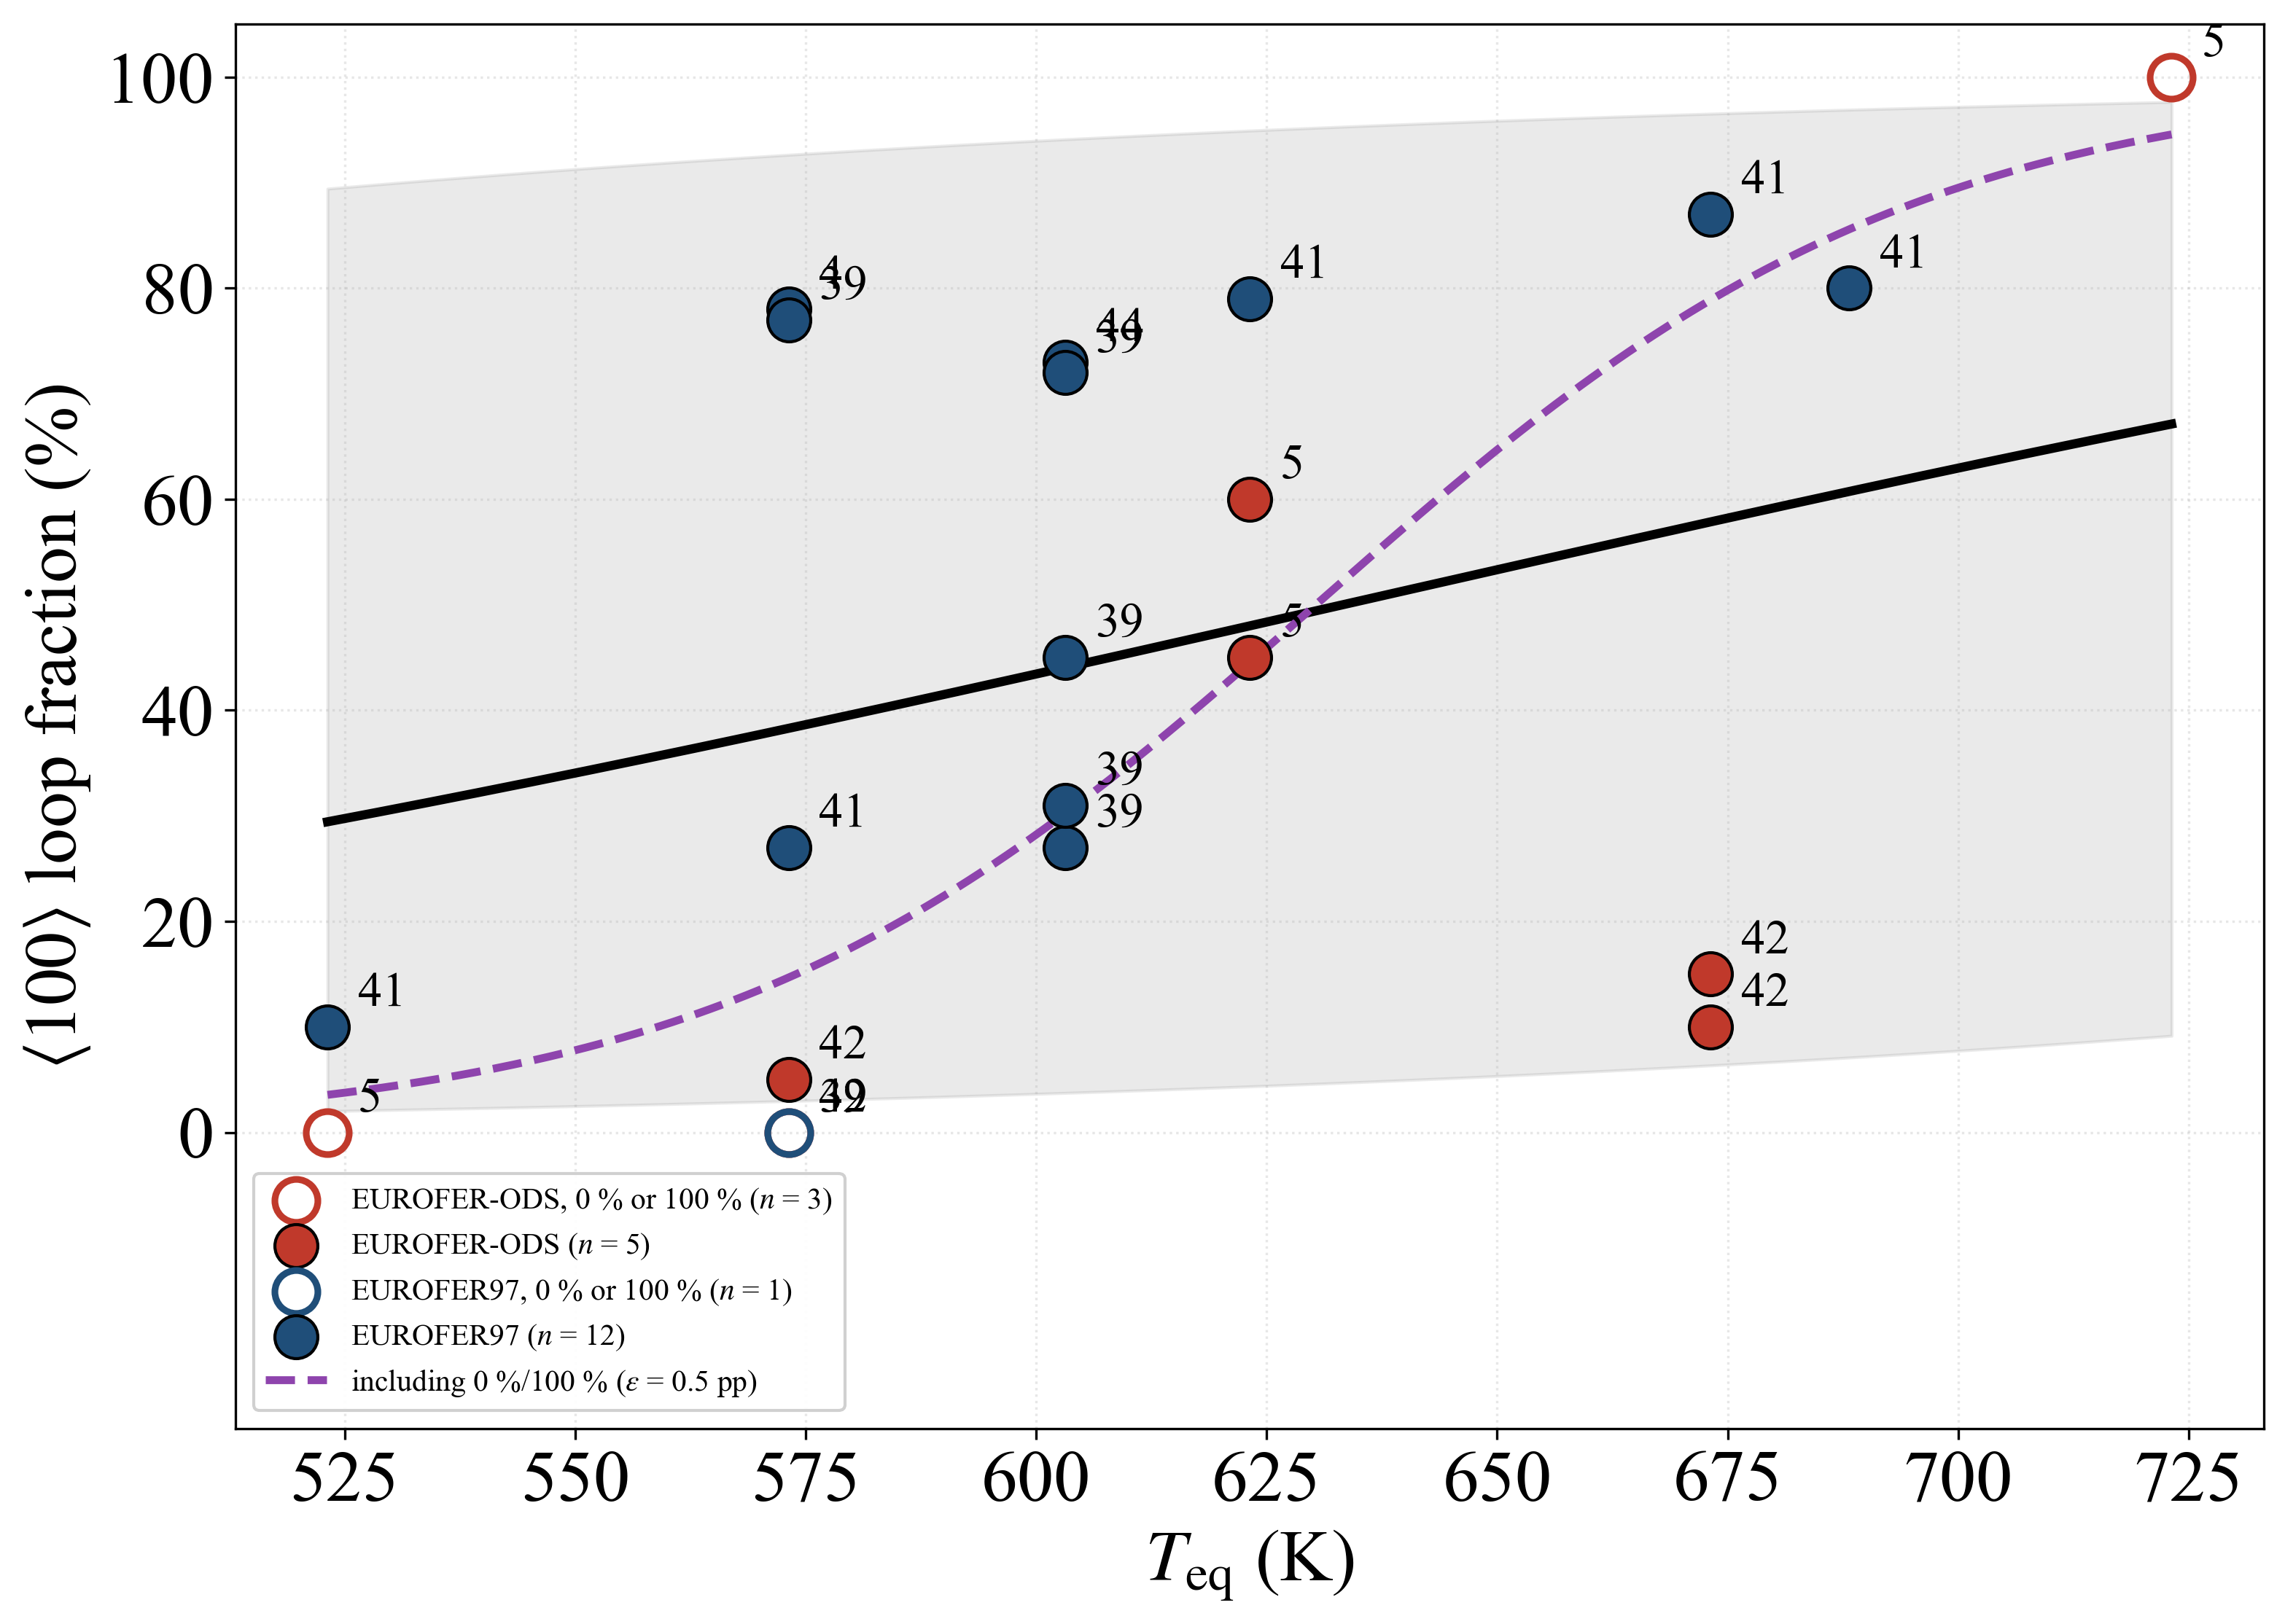
\includegraphics[width=\linewidth]{figures/experiments/loop_fraction_neutron_T.png}
  \caption{$\langle 100\rangle$ loop fraction after neutron irradiation, against
  equivalent temperature. Filled symbols are measurements strictly between $0$ and
  $100\,\%$ and carry the solid logistic fit of Eq.~\eqref{eq:logit} with its $\pm 2s$
  band; open symbols are the four measurements reporting exactly $0\,\%$ or $100\,\%$,
  which are plotted but not fitted. The dashed purple curve is the sensitivity fit that
  includes them under a $0.5$~pp continuity correction. Colour separates EUROFER97 from
  EUROFER-ODS; labels are the source numbers of Table~\ref{tab:lf-refs}. The pooled
  trend is not resolved, and the difference between the two curves is the honest
  measure of how much of it is an encoding artefact.}
  \label{fig:lf-n}
\end{figure}

\subsubsection*{Ion irradiation}

The ion set (Figure~\ref{fig:lf-i}) is too small to fit: five measurements from two
sources at effectively two temperatures, giving $b = 1.6\times10^{-2} \pm
2.4\times10^{-2}$~K$^{-1}$ ($t = 0.68$). What it does show, at fixed temperature and
dose, is a strong \emph{microstructural} effect. Brimbal (2015) reports, at
$400~^{\circ}$C and $26$~dpa in one experiment, $87\,\%$ $\langle 100\rangle$ in
EUROFER97, $76\,\%$ in the tempered-martensite grains of EUROFER-ODS and $32\,\%$ in
its ferrite grains --- a factor of nearly three in the odds ratio between two grain
types of the same specimen. Whatever sets the loop character responds more strongly to
local microstructure than the pooled temperature trend does, which is a caution against
calibrating a conversion model on a single alloy condition.

\begin{figure}[htbp]
  \centering
  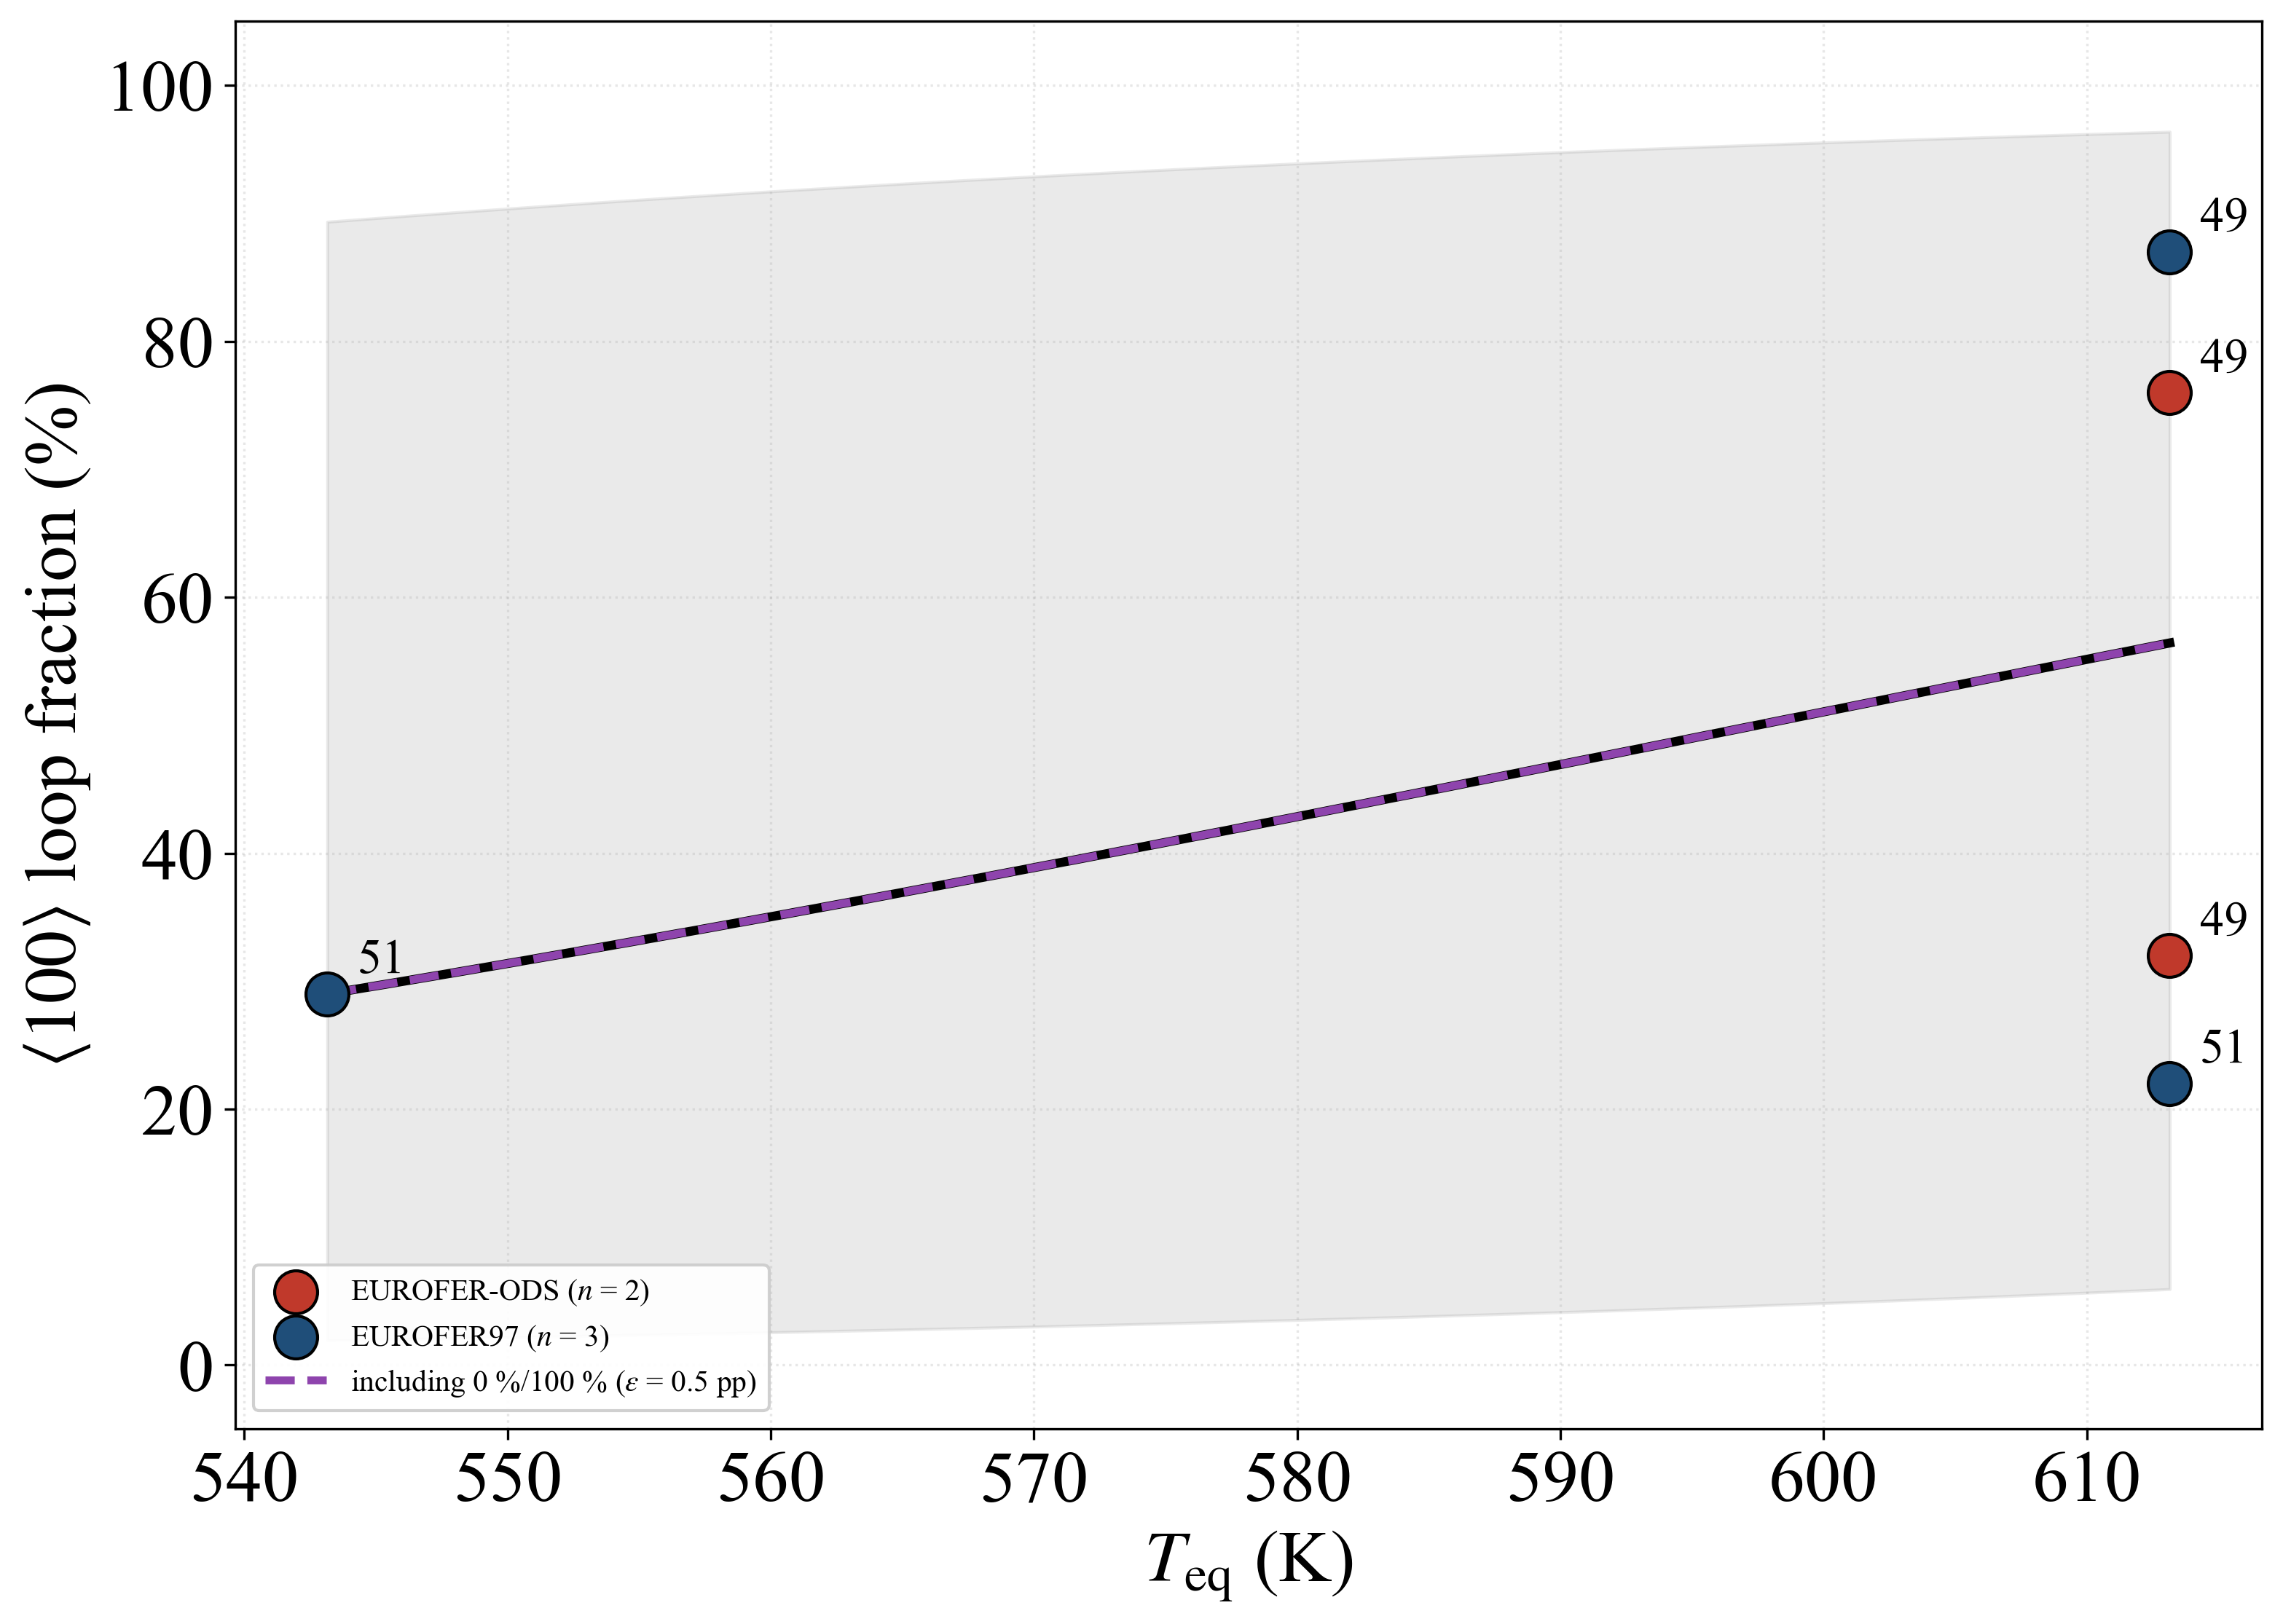
\includegraphics[width=\linewidth]{figures/experiments/loop_fraction_ion_T.png}
  \caption{$\langle 100\rangle$ loop fraction after ion irradiation. Five measurements
  at two equivalent temperatures; the fit is shown for completeness and is not
  resolved. The three points at $613$~K are one experiment (source 49) on EUROFER97 and
  on the two grain populations of EUROFER-ODS, and span $32$--$87\,\%$.}
  \label{fig:lf-i}
\end{figure}

\subsubsection*{Holding the alloy fixed: EUROFER97 alone}

Ten of the $26$ measurements are EUROFER-ODS, and pooling them with the unstrengthened
steel is not a small approximation. The oxide dispersion acts directly on the loop
population --- it provides a dense array of particle interfaces that trap gliding
$\frac{1}{2}\langle 111\rangle$ loops before they can interact with one another ---
so the two alloy classes pose different problems, and Figures~\ref{fig:lf-n}
and~\ref{fig:lf-i} mix them. Restricting to EUROFER97 leaves $16$ measurements, $13$
neutron and three ion, from six sources, and the neutron fit changes character
entirely (Figure~\ref{fig:lf-n-97}):

\begin{center}
\begin{tabular}{lrr}
\toprule
Neutron, interior points only & All alloys & EUROFER97 only \\
\midrule
$n$                        & 17                  & 12 \\
$b$ (K$^{-1}$)             & $+0.0079 \pm 0.0085$ & $+0.0188 \pm 0.0071$ \\
$t$                        & 0.94                & 2.66 \\
$R^2$                      & 0.056               & 0.415 \\
$s$ (logit units)          & 1.50                & 1.04 \\
$T_{50}$ ($^{\circ}$C)     & 360                 & 313 \\
\bottomrule
\end{tabular}
\end{center}

The trend that could not be resolved across both alloy classes is resolved at
$2.7\sigma$ once the material is held fixed; the residual scatter falls by a third,
and $T_{50}$ moves down to $313~^{\circ}$C --- within $20~^{\circ}$C of the
$331~^{\circ}$C obtained from the single Klimenkov (2020) series, which is as close an
agreement as this database offers anywhere.

A second improvement matters more than the gain in $R^2$. Only one of the $13$
retained neutron measurements is a boundary value, so the continuity correction that
dominated the all-alloy panel no longer does: the solid and dashed curves of
Figure~\ref{fig:lf-n-97} very nearly coincide ($T_{50} = 313$ against
$333~^{\circ}$C, where the all-alloy panel gave $360$ against $357~^{\circ}$C from the
same pair of fits). The EUROFER97 result therefore does not depend on how the
qualitative $0\,\%$ and $100\,\%$ entries are encoded, and it is the fit to use as a
calibration target.

The ion subset does not survive the restriction. Three measurements at two equivalent
temperatures remain (Figure~\ref{fig:lf-i-97}), and the two at $613$~K are $22\,\%$
and $87\,\%$ --- from different laboratories at the same nominal condition. The fit
returns $t = 0.44$ and a prediction band spanning almost the full axis; it is
reproduced for completeness and carries no constraint.

\begin{figure}[htbp]
  \centering
  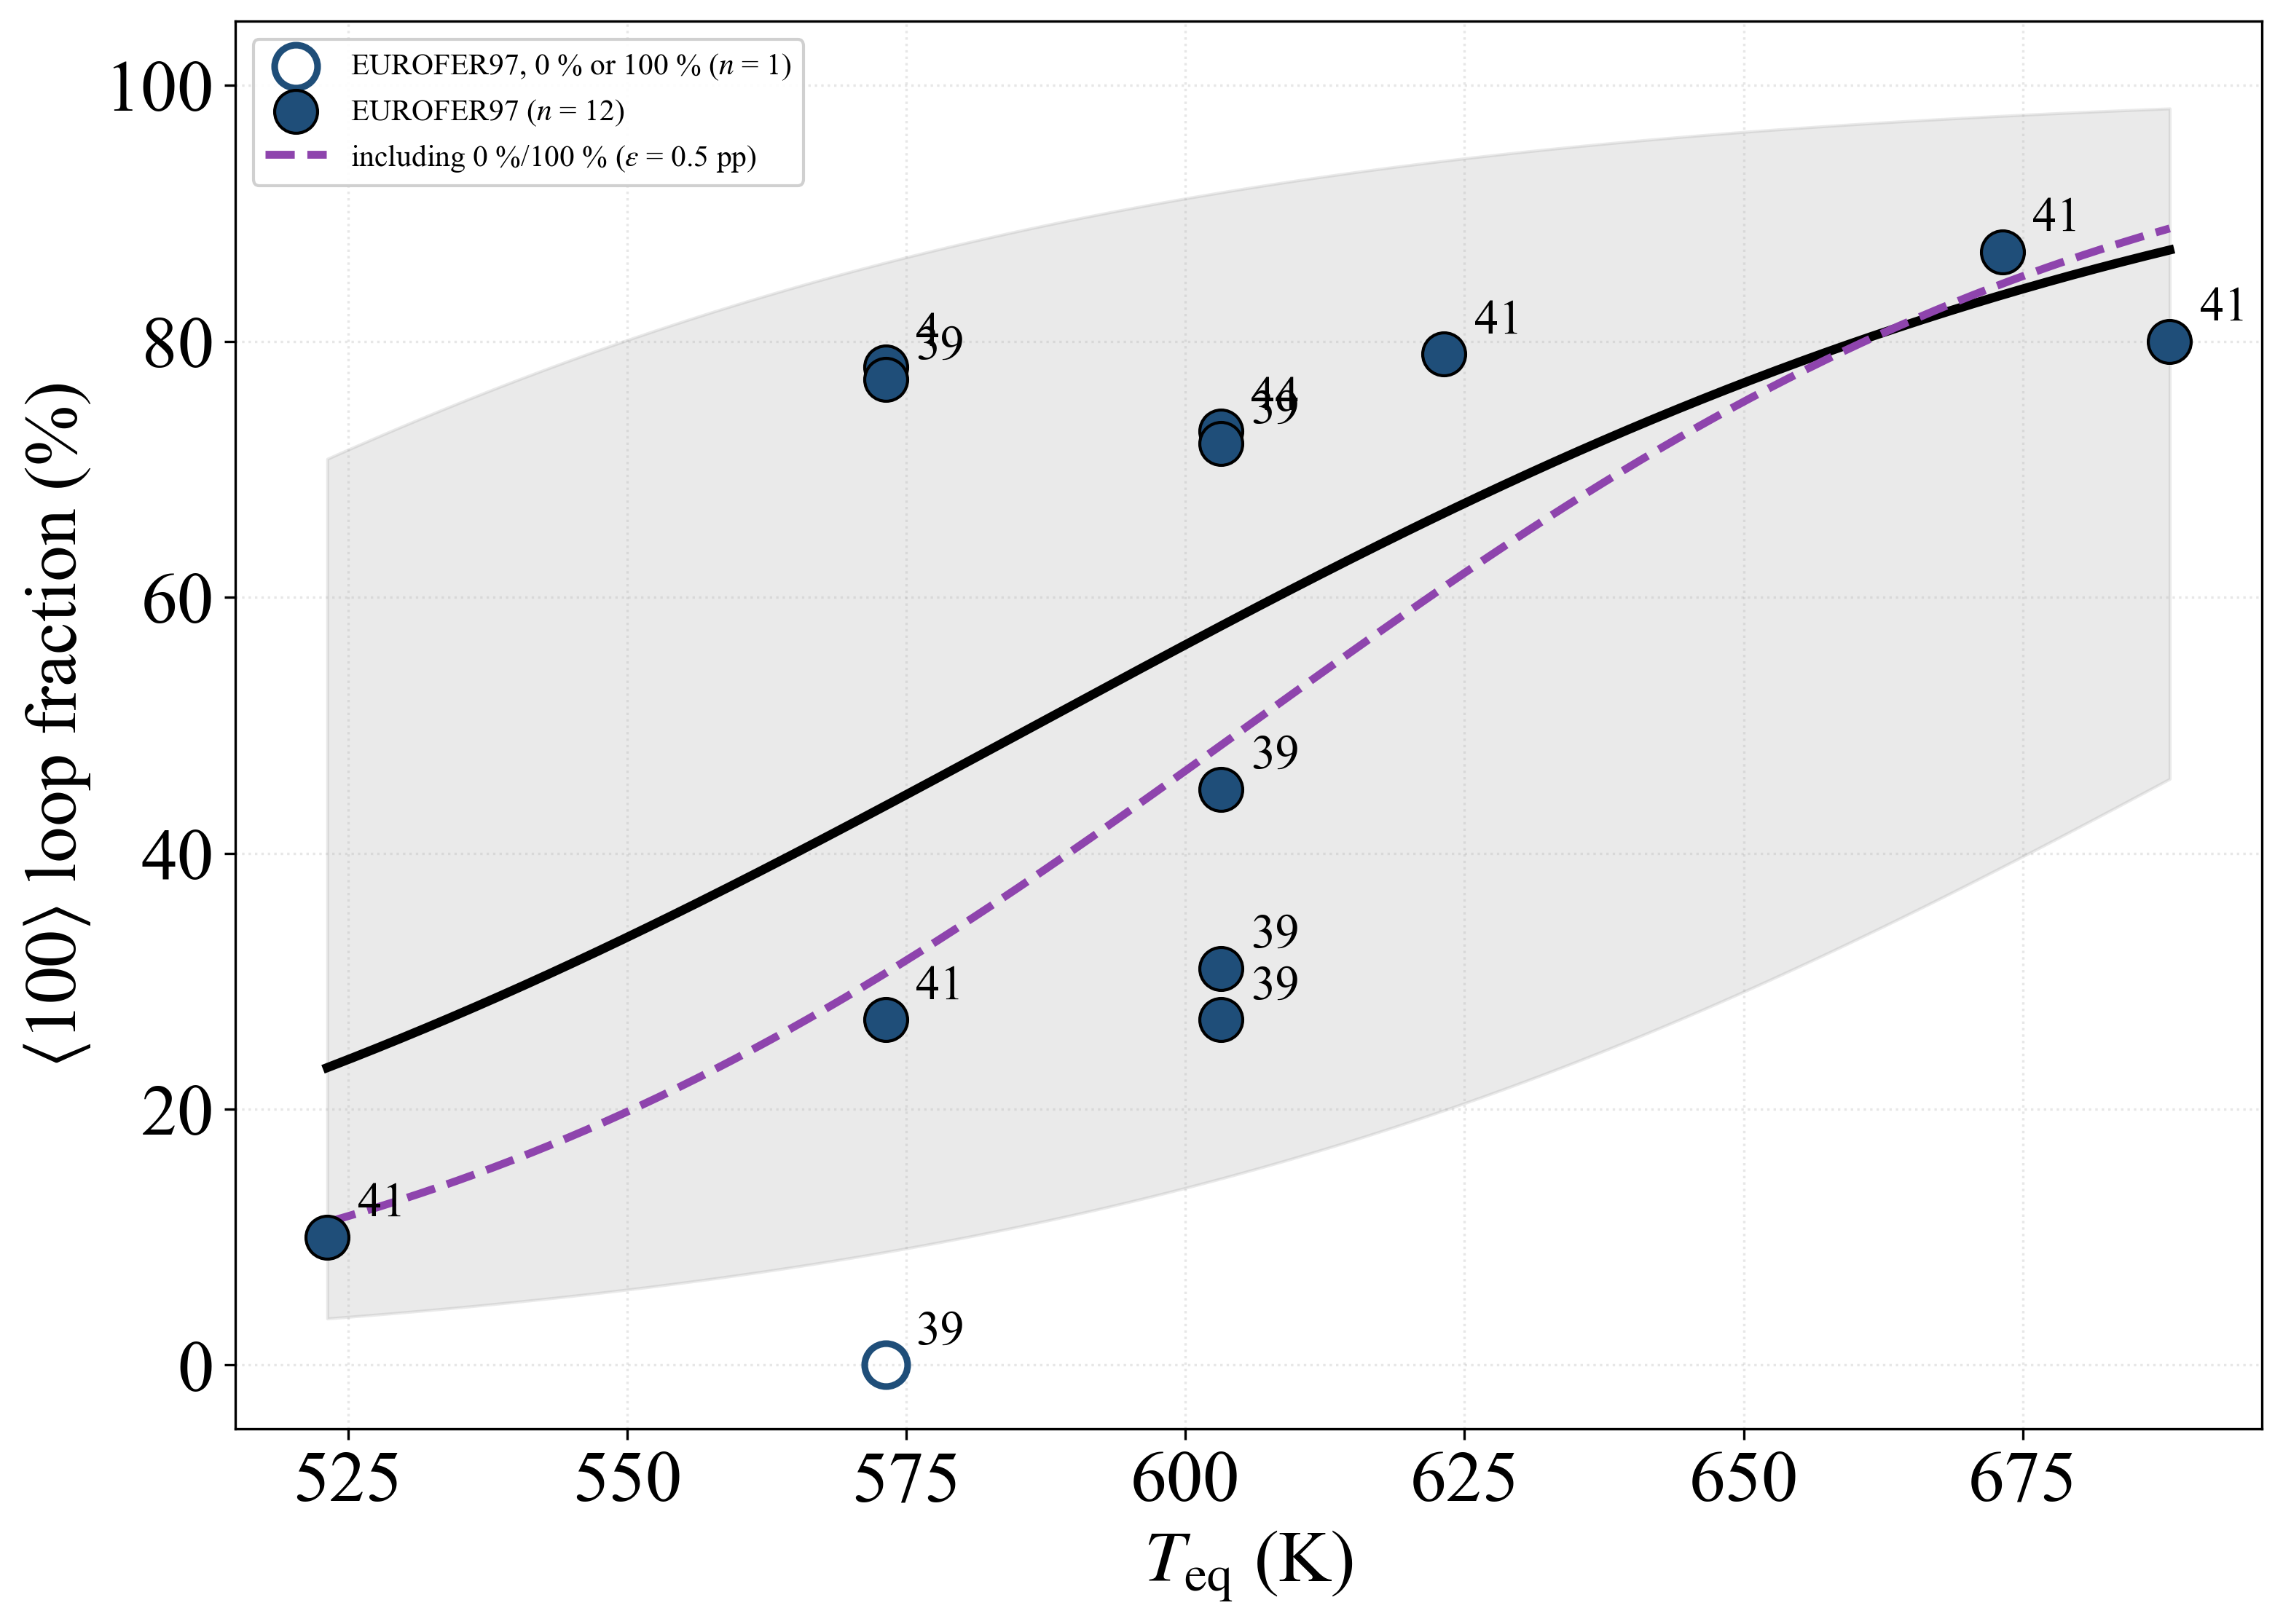
\includegraphics[width=\linewidth]{figures/experiments/loop_fraction_neutron_T_eurofer97.png}
  \caption{$\langle 100\rangle$ loop fraction after neutron irradiation of EUROFER97
  alone, the EUROFER-ODS measurements of Figure~\ref{fig:lf-n} having been removed.
  Symbols, curves and band are as in Figure~\ref{fig:lf-n}. Holding the alloy fixed
  resolves the temperature dependence ($t = 2.66$, $R^2 = 0.415$,
  $T_{50} = 313~^{\circ}$C) and, because only one boundary measurement remains, brings
  the solid fit and the dashed continuity-corrected fit almost into coincidence --- so
  unlike Figure~\ref{fig:lf-n} the result no longer turns on how the qualitative
  entries are encoded.}
  \label{fig:lf-n-97}
\end{figure}

\begin{figure}[htbp]
  \centering
  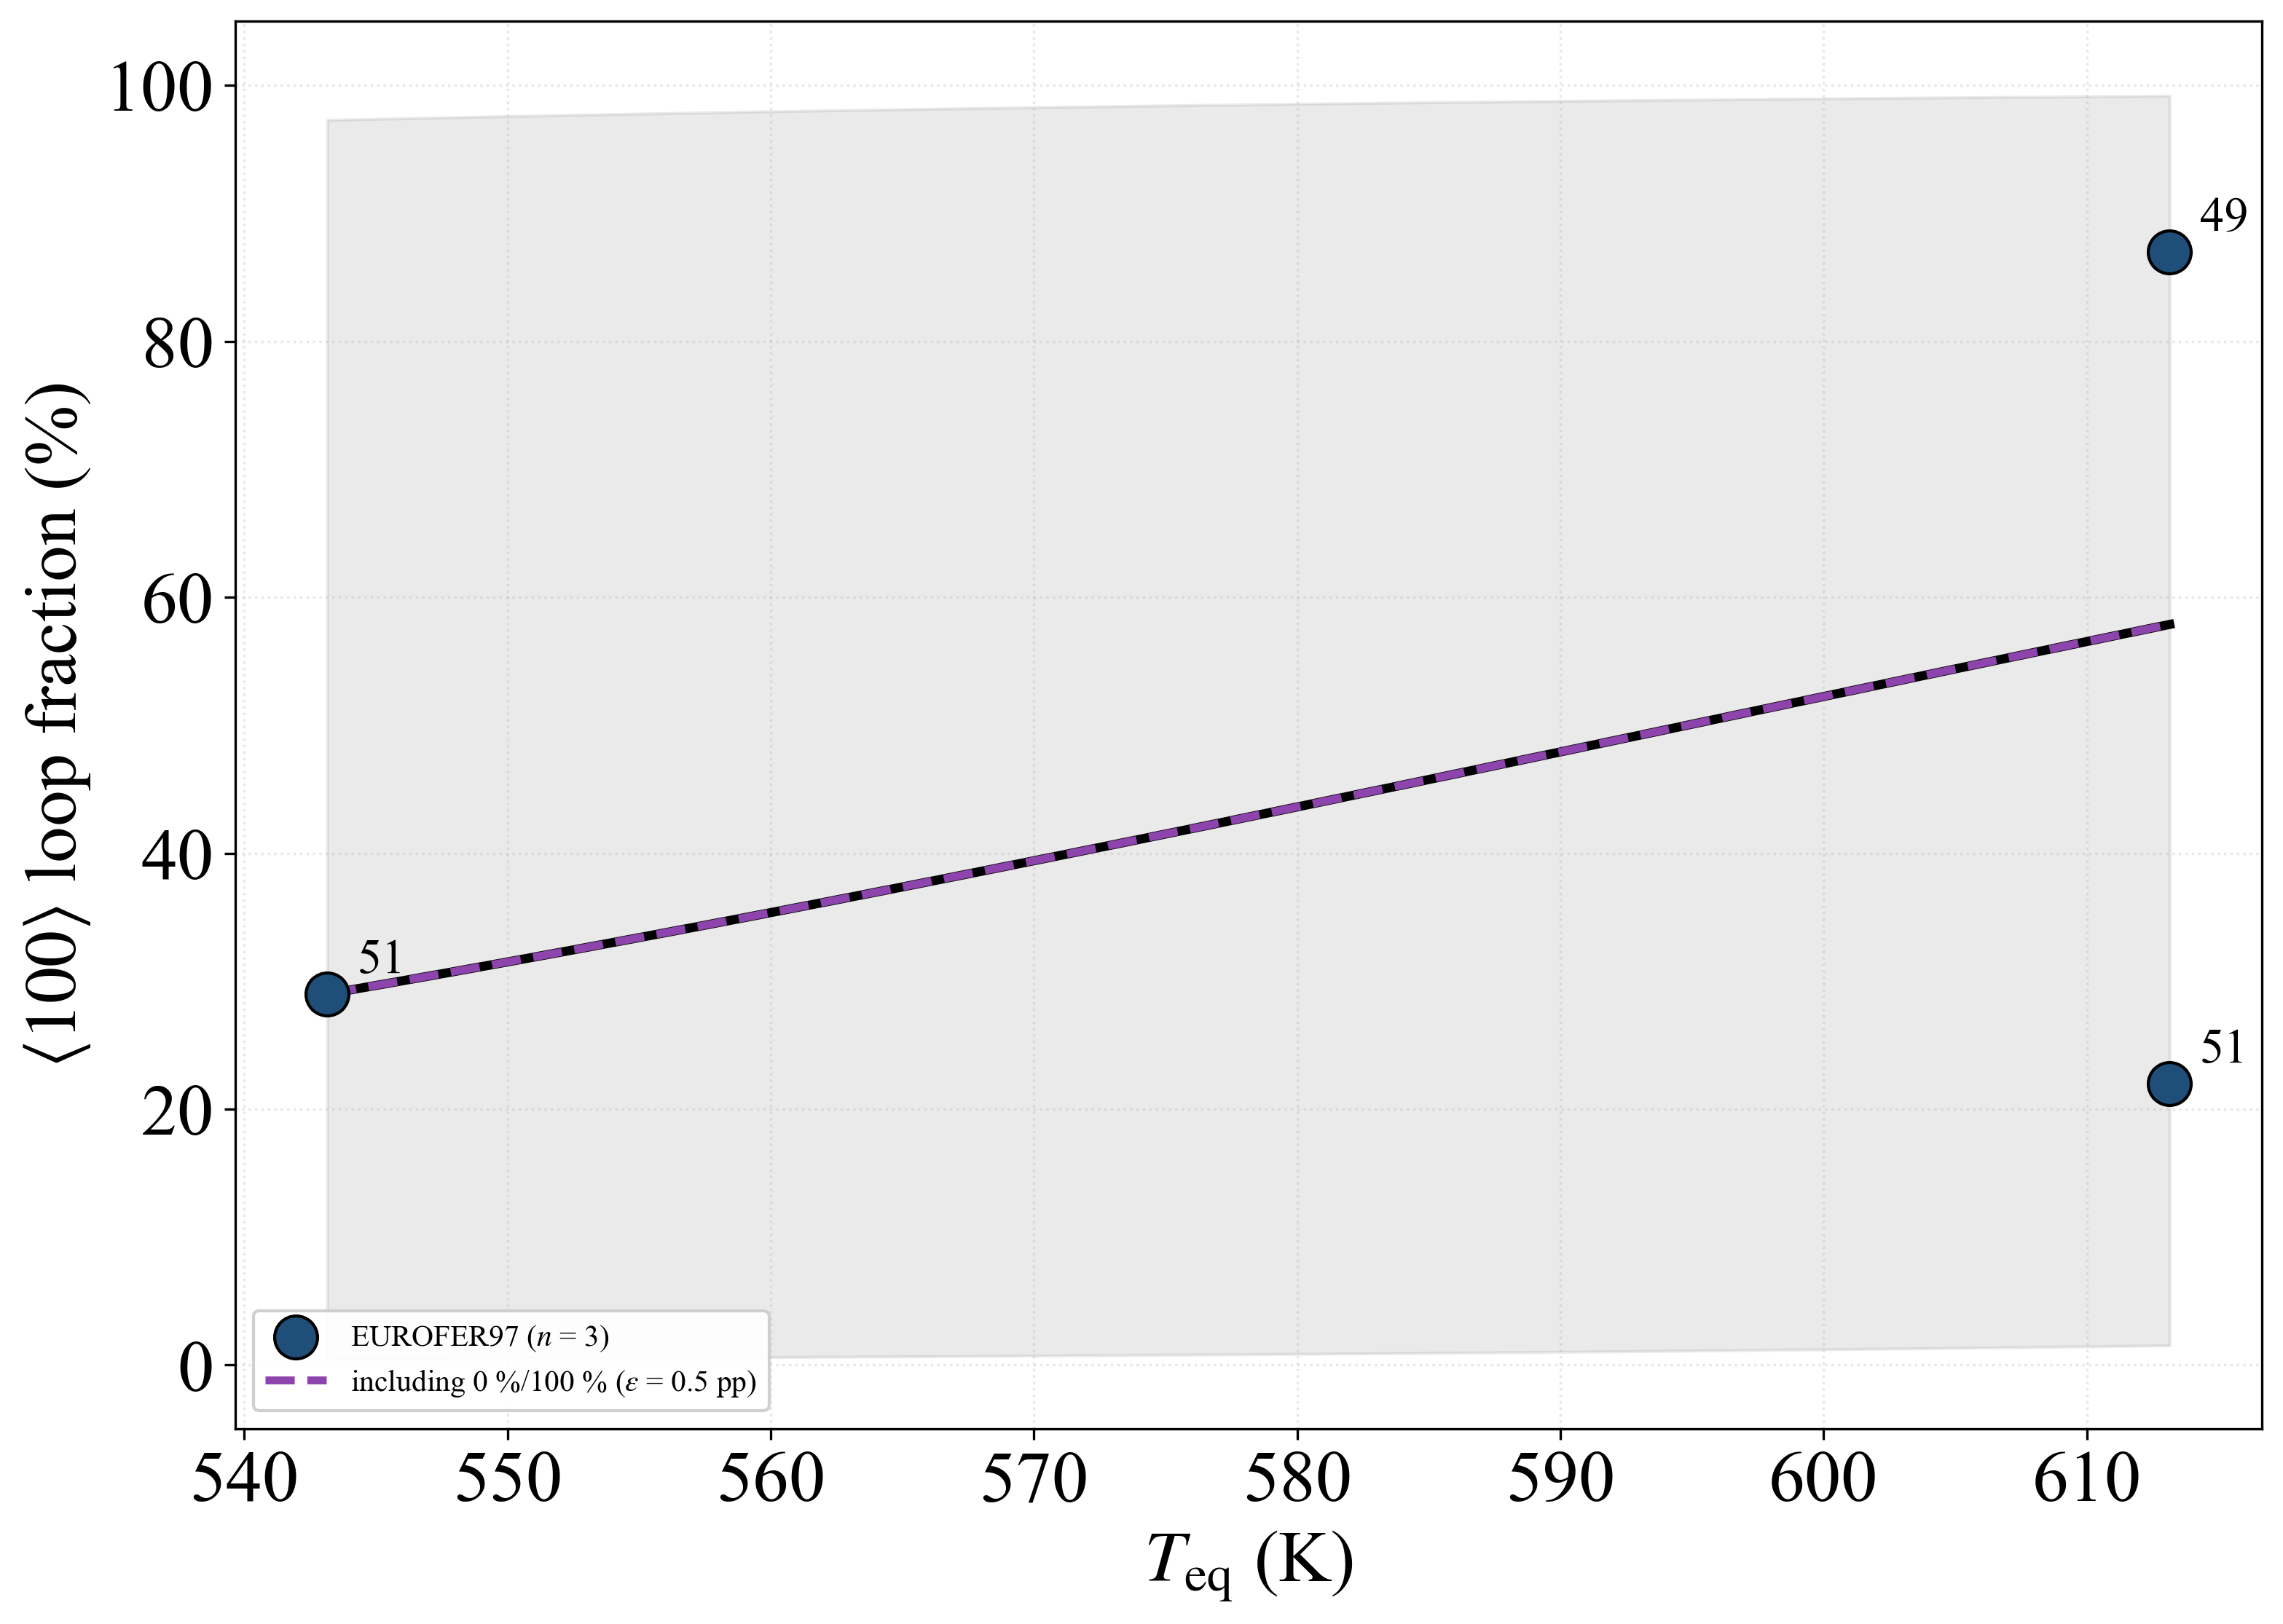
\includegraphics[width=\linewidth]{figures/experiments/loop_fraction_ion_T_eurofer97.png}
  \caption{The ion measurements of Figure~\ref{fig:lf-i} restricted to EUROFER97:
  three points at two equivalent temperatures, of which the two at $613$~K differ by a
  factor of four in the odds ratio. The fit ($t = 0.44$) and its $\pm 2s$ band, which
  spans nearly the whole axis, are shown to make the absence of a constraint explicit
  rather than to be read as a trend.}
  \label{fig:lf-i-97}
\end{figure}

\subsubsection*{Where the trend actually lives}

The pooled panels understate the data badly, and Figure~\ref{fig:lf-by-source} shows
why: within a single study the temperature dependence is strong and consistent, and it
is the offsets \emph{between} studies that destroy it. Fitting each source separately,
\begin{center}
\begin{tabular}{llrrrr}
\toprule
Source & Material & $n$ & $b$ (K$^{-1}$) & $R^2$ & $T_{50}$ ($^{\circ}$C) \\
\midrule
{[41]} Klimenkov 2020 & EUROFER97     & 5 & $+0.0245 \pm 0.0048$ & 0.895 & 331 \\
{[42]} Klimenkov 2021 & EUROFER-ODS   & 3 & $+0.0098 \pm 0.0040$ & 0.856 & 601 \\
{[39]} Dethloff 2018  & EUROFER97     & 5 & $-0.0490 \pm 0.0325$ & 0.431 & 325 \\
\bottomrule
\end{tabular}
\end{center}
Klimenkov (2020) traces the fraction from $10\,\%$ at $250~^{\circ}$C to $87\,\%$ at
$400~^{\circ}$C in one alloy on one instrument, giving $t = 5.1$ and $T_{50} =
331~^{\circ}$C; Klimenkov (2017) traces the ODS variant from $0\,\%$ at
$250~^{\circ}$C to $100\,\%$ at $450~^{\circ}$C. The Dethloff (2018) series runs the
other way, but all five of its points lie within $30~^{\circ}$C of each other, so its
slope is an artefact of the analysis spread at essentially one temperature rather than a
temperature trend --- which is exactly what the vertical red segments in
Figure~\ref{fig:lf-by-source} represent. Figure~\ref{fig:lf-by-source-97} repeats the
comparison for EUROFER97 alone, where only those two studies remain.

One further discrepancy must be carried with any use of these data, and unlike source
40 it cannot be set aside, because both readings are legitimate.

\begin{itemize}
\item \textbf{Black dots.} Dethloff (2018) reports each condition twice, once counting
  resolved loops only and once including black-dot damage. The fraction moves from
  $72\,\%$ to $45\,\%$ at $330~^{\circ}$C and $15$~dpa, and from $27\,\%$ to $31\,\%$
  at $32$~dpa. A $27$ percentage-point swing from a counting convention, at one
  condition in one laboratory, is comparable to the entire pooled temperature signal.
  Any comparison against a model must state whether the model's small-loop cutoff
  corresponds to the black-dot-inclusive count or not.
\end{itemize}

\begin{figure}[htbp]
  \centering
  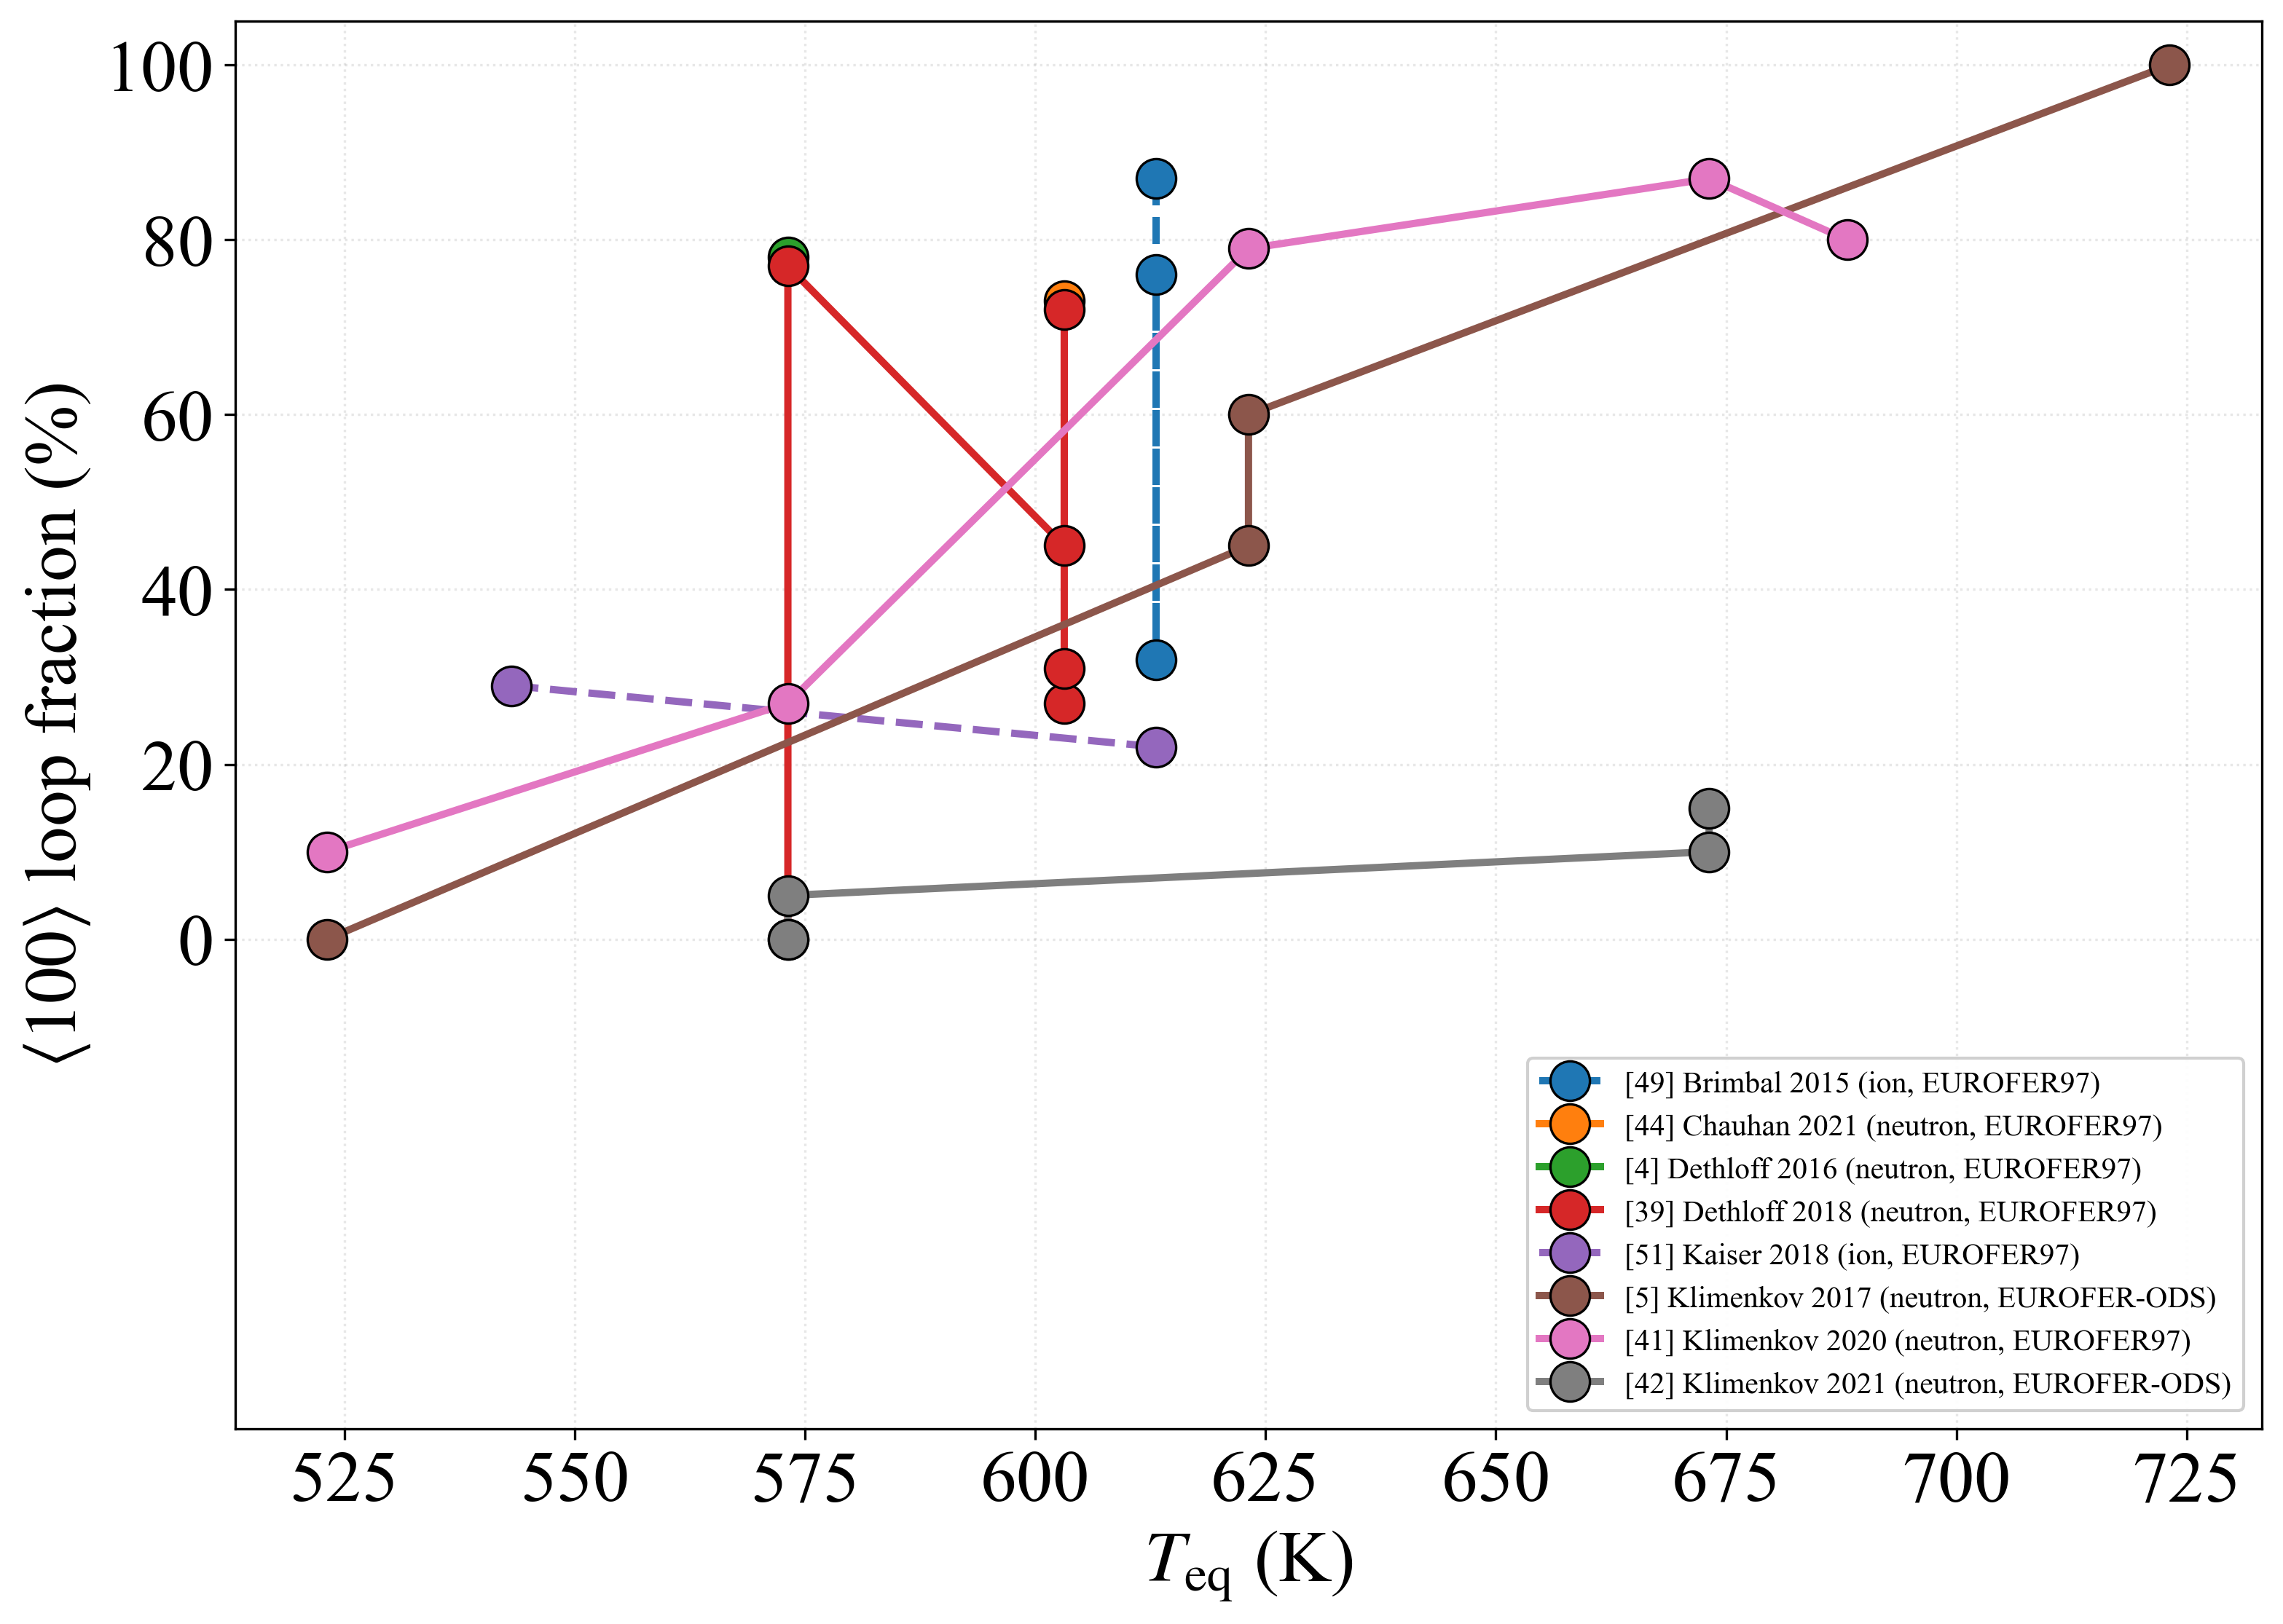
\includegraphics[width=\linewidth]{figures/experiments/loop_fraction_by_source.png}
  \caption{The same measurements, joined within each source and ordered by
  temperature; solid lines are neutron irradiations, dashed lines ion irradiations.
  Within a study the rise with temperature is steep and consistent (sources 41 and 5);
  the between-study offsets are what flatten the pooled fit of
  Figure~\ref{fig:lf-n}. \emph{Vertical segments are not trends}: they join
  measurements made at one temperature, either two analyses of one specimen (source 39,
  with and without black dots) or different grain populations of one experiment
  (source 49).}
  \label{fig:lf-by-source}
\end{figure}

\begin{figure}[htbp]
  \centering
  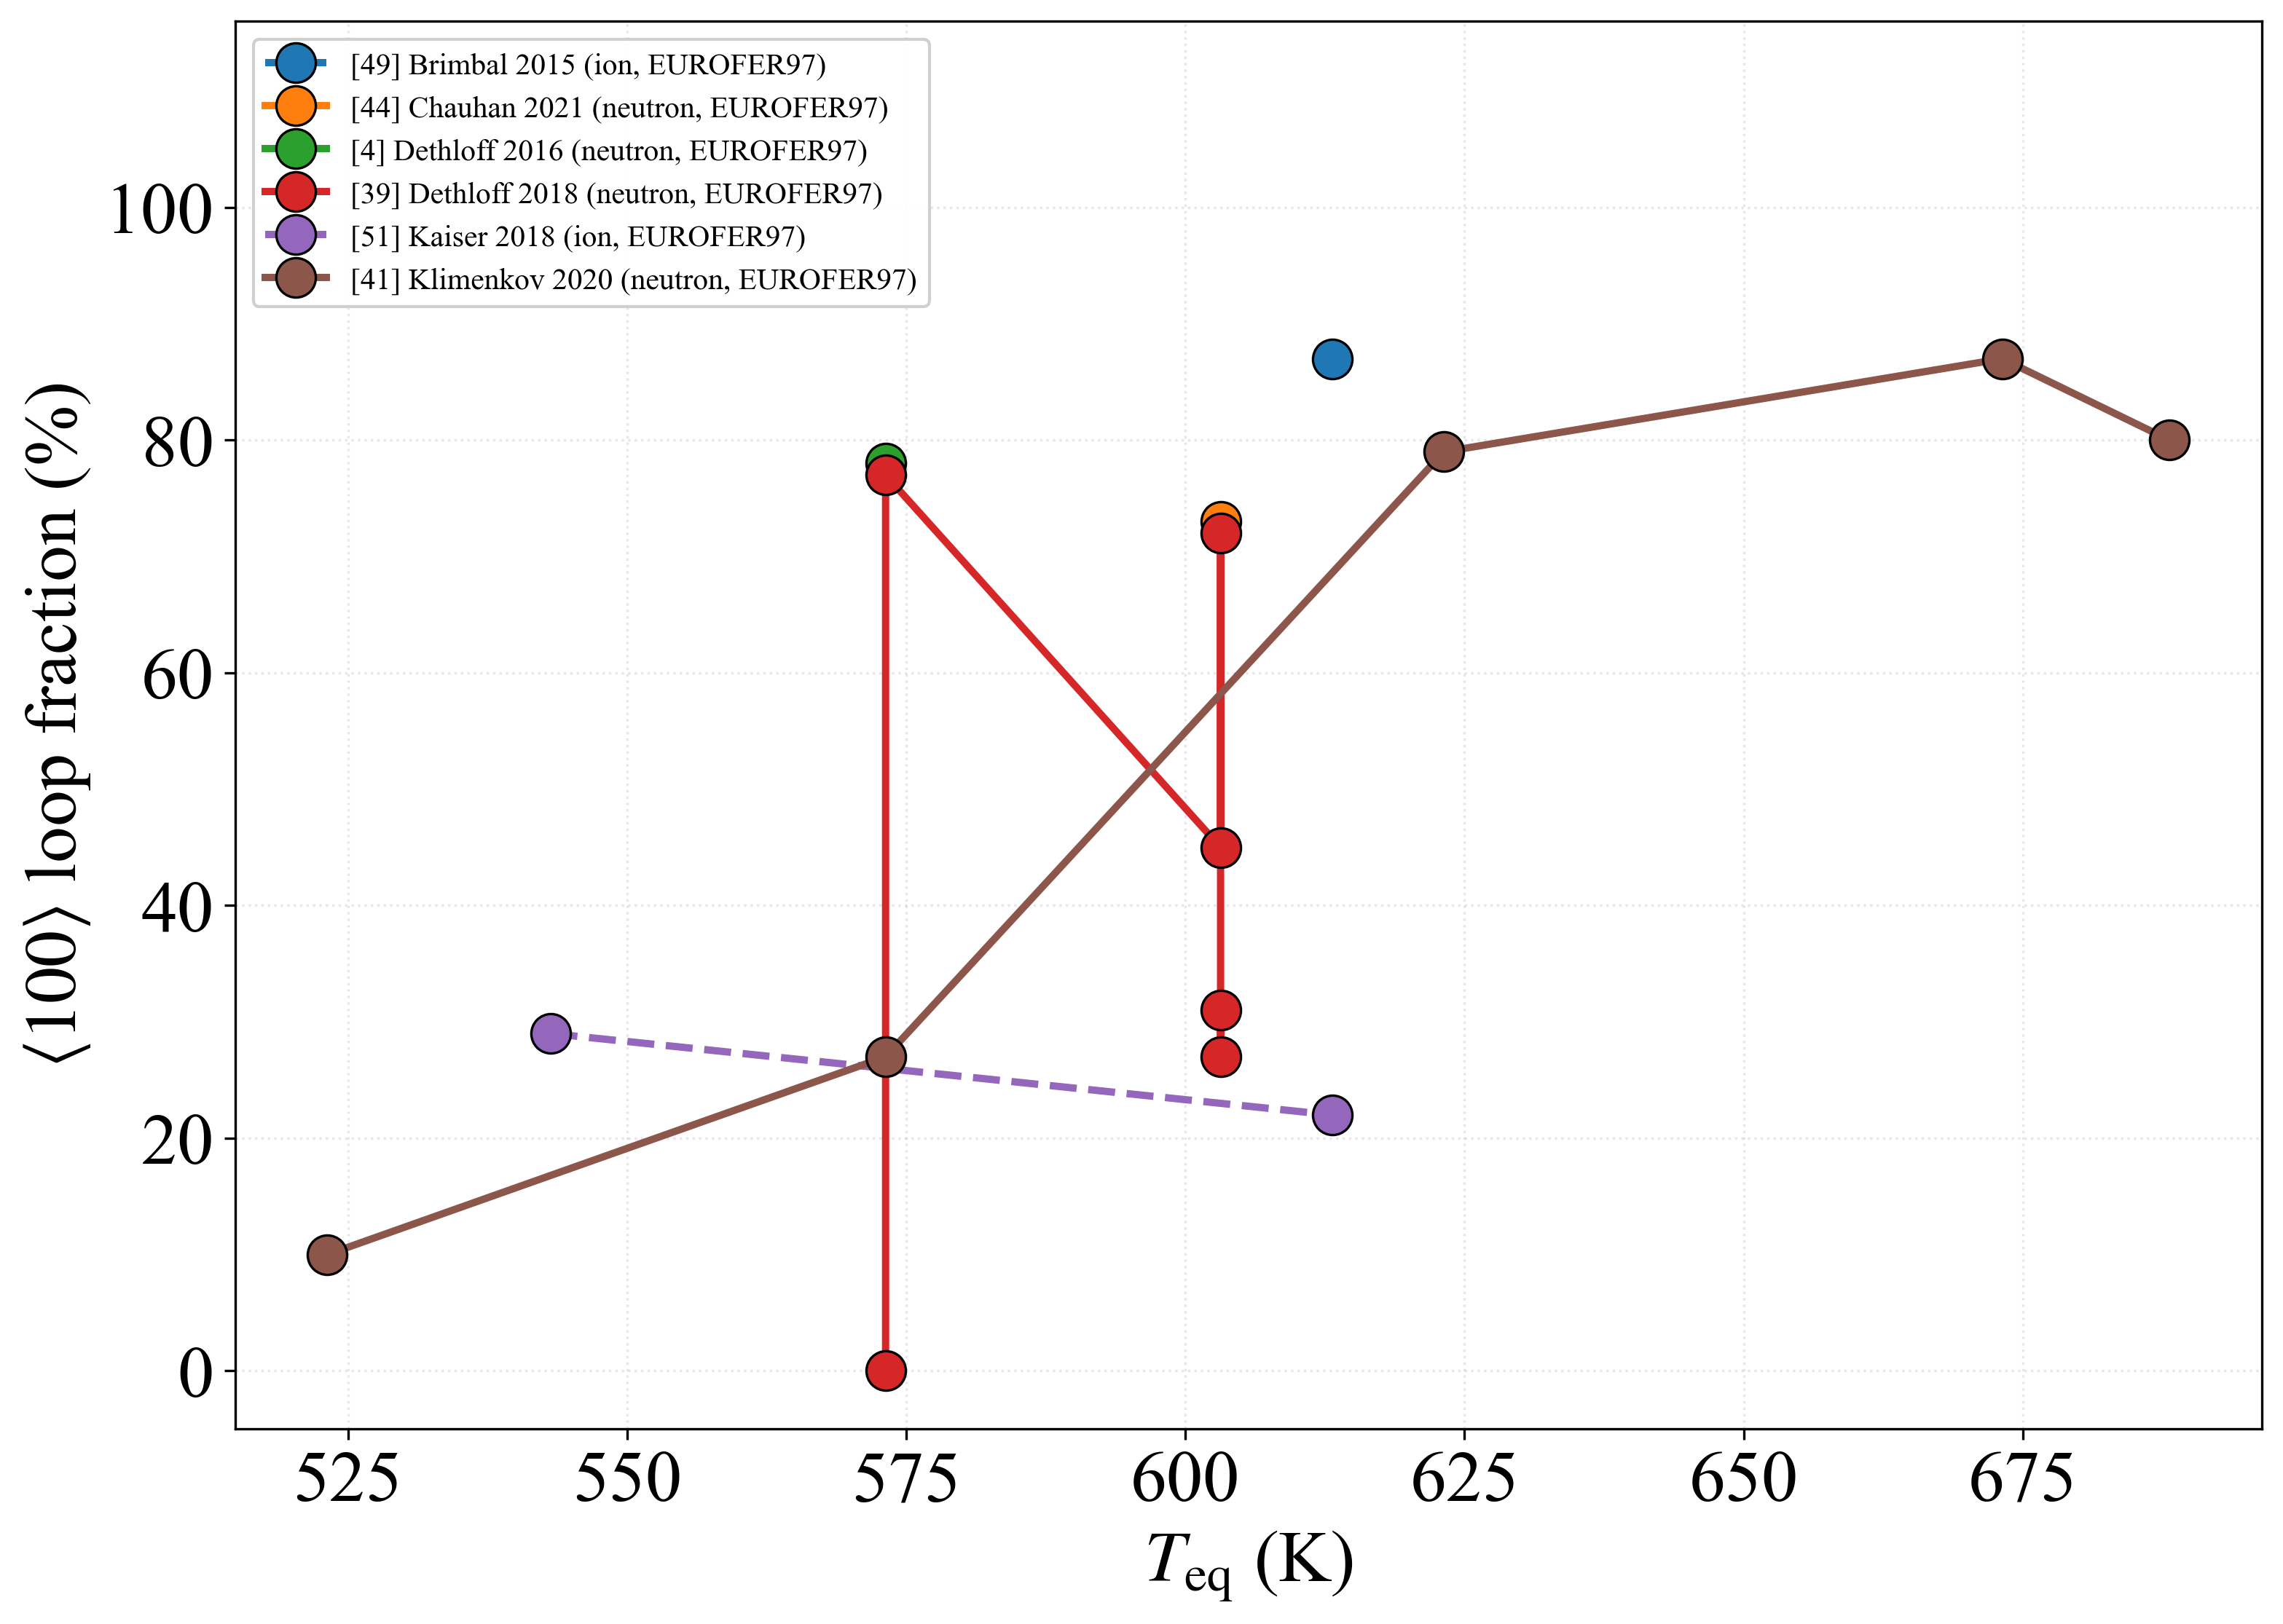
\includegraphics[width=\linewidth]{figures/experiments/loop_fraction_by_source_eurofer97.png}
  \caption{Figure~\ref{fig:lf-by-source} restricted to EUROFER97. With the ODS series
  removed, only two neutron studies span more than one temperature, and they disagree:
  Klimenkov (2020) rises from $10$ to $87\,\%$ across $165~^{\circ}$C, while the whole
  Dethloff (2018) set lies within $30~^{\circ}$C and its apparent negative slope is the
  spread between analyses of one specimen rather than a temperature trend. The
  EUROFER97 fit of Figure~\ref{fig:lf-n-97} is essentially the Klimenkov series with
  the Dethloff scatter superposed.}
  \label{fig:lf-by-source-97}
\end{figure}

\subsubsection*{What to take from this section}

The $\langle 100\rangle$ fraction rises with irradiation temperature, strongly and
reproducibly \emph{within} a given study, and passes through $50\,\%$ near
$310$--$330~^{\circ}$C in EUROFER97 at $13$--$18$~dpa. That crossover, not the pooled
slope, is the number worth calibrating against, and its uncertainty is set by the
between-laboratory spread rather than by counting statistics. Two independent routes
agree on it: the EUROFER97-only fit of Figure~\ref{fig:lf-n-97} gives
$T_{50} = 313~^{\circ}$C and the single Klimenkov (2020) series gives
$331~^{\circ}$C. The all-alloy fit of Figure~\ref{fig:lf-n} should not be used for
this purpose --- its slope is not resolved, and what it mostly measures is the
difference between EUROFER97 and EUROFER-ODS. In EUROFER-ODS the
crossover is displaced upward --- source 42 puts it near $600~^{\circ}$C --- consistent
with the oxide dispersion suppressing the $\frac{1}{2}\langle 111\rangle$ interactions
that produce $\langle 100\rangle$ loops, though with three points that reading is
suggestive rather than established.

\begin{table}[htbp]
\centering\small
\caption{The $26$ retained $\langle 100\rangle$-fraction measurements; the two
measurements of source 40 are excluded, as described in the text. ``\#'' is the source
number of Table~\ref{tab:lf-refs}; ``irr.'' is n for neutron and i for ion;
$T_{\rm eq}$ is the equivalent temperature of Eq.~\eqref{eq:tshift}. Entries marked
$^{\rm bd}$ are the black-dot-inclusive counts of source 39, reported alongside the
resolved-loop counts for the same specimen. The four entries at $0$ or $100\,\%$ are
qualitative statements and are excluded from the quoted fits.}
\label{tab:lf-data}
\begin{tabular}{rlcrrrr}
\toprule
\# & Material & irr. & $T$ ($^{\circ}$C) & $T_{\rm eq}$ (K) & Dose (dpa) &
$f_{\langle 100\rangle}$ (\%) \\
\midrule
4 & EUROFER97 & n & 300 & 573 & 15 & 78 \\
5 & EUROFER-ODS & n & 250 & 523 & 16.2 & 0 \\
5 & EUROFER-ODS & n & 350 & 623 & 16.2 & 45 \\
5 & EUROFER-ODS & n & 350 & 623 & 16.2 & 60 \\
5 & EUROFER-ODS & n & 450 & 723 & 16.2 & 100 \\
39 & EUROFER97 & n & 300 & 573 & 15 & 0 \\
39 & EUROFER97 & n & 300 & 573 & 15 & 77 \\
39 & EUROFER97 & n & 330 & 603 & 15 & 72 \\
39 & EUROFER97 & n & 330 & 603 & 15 & 45$^{\rm bd}$ \\
39 & EUROFER97 & n & 330 & 603 & 32 & 27 \\
39 & EUROFER97 & n & 330 & 603 & 32 & 31$^{\rm bd}$ \\
41 & EUROFER97 & n & 250 & 523 & 13.4 & 10 \\
41 & EUROFER97 & n & 300 & 573 & 14.6 & 27 \\
41 & EUROFER97 & n & 350 & 623 & 17.4 & 79 \\
41 & EUROFER97 & n & 400 & 673 & 17.2 & 87 \\
41 & EUROFER97 & n & 415 & 688 & 18.1 & 80 \\
42 & EUROFER-ODS & n & 300 & 573 & 16.2 & 0 \\
42 & EUROFER-ODS & n & 300 & 573 & 16.2 & 5 \\
42 & EUROFER-ODS & n & 400 & 673 & 16.2 & 10 \\
42 & EUROFER-ODS & n & 400 & 673 & 16.2 & 15 \\
44 & EUROFER97 & n & 330 & 603 & 15 & 73 \\
49 & EUROFER97 & i & 400 & 613 & 26 & 87 \\
49 & EUROFER-ODS (t.\,mart.) & i & 400 & 613 & 26 & 76 \\
49 & EUROFER-ODS (ferrite) & i & 400 & 613 & 26 & 32 \\
51 & EUROFER97 & i & 330 & 543 & 16 & 29 \\
51 & EUROFER97 & i & 400 & 613 & 16 & 22 \\
\bottomrule
\end{tabular}
\end{table}

\begin{table}[htbp]
\centering\small
\caption{Sources introduced by the \texttt{Loop\_fractions} sheet. Unlike the five
defect-population sheets, this one records its sources as titles and carries no DOI
column; author, year and title below are reproduced from the workbook and the journal
was not independently resolved, so nothing is asserted that the sheet does not state.
Numbering continues that of Table~\ref{tab:refs}, so a paper appearing in both keeps
one number throughout. A dagger marks the eight sources whose
$\langle 100\rangle$ fractions are analysed here; a double dagger marks source 40,
which reports fractions that are set aside for the reason given in the text; the
remainder contribute total-loop rows only.}
\label{tab:lf-refs}
\begin{tabular}{rll}
\toprule
\# & Source & Title as recorded in the workbook \\
\midrule
 4$^{\dagger}$ & Dethloff 2016   & (Table~\ref{tab:refs}) Microstructural defects in EUROFER 97 after \\
                &                & different neutron irradiation conditions \\
 5$^{\dagger}$ & Klimenkov 2017  & (Table~\ref{tab:refs}) Effect of irradiation temperature on the \\
                &                & microstructure of a ferritic--martensitic ODS steel \\
25              & Boulanger \& Serruys 2009 & (Table~\ref{tab:refs}) Dislocation loops in Eurofer and an \\
                &                & Fe--Cr alloy irradiated by ions at 350 and 550\,$^{\circ}$C \\
39$^{\dagger}$ & Dethloff 2018   & Review and critical assessment of dislocation loop analyses \\
                &                & on EUROFER 97 \\
40$^{\ddagger}$ & Klimenkov 2011  & Characterization of radiation induced defects in EUROFER 97 \\
                &                & after neutron irradiation \\
41$^{\dagger}$ & Klimenkov 2020  & Correlation of microstructural and mechanical properties of \\
                &                & neutron irradiated EUROFER97 steel \\
42$^{\dagger}$ & Klimenkov 2021  & Post-irradiation microstructural examination of EUROFER-ODS \\
                &                & steel irradiated at 300 and 400\,$^{\circ}$C \\
43              & Wei\ss{} 2012   & Quantitative characterization of microstructural defects in \\
                &                & up to 32 dpa neutron irradiated EUROFER97 \\
44$^{\dagger}$ & Chauhan 2021    & Post-irradiation annealing of neutron-irradiated EUROFER97 \\
45              & Sch\"aublin 2002 & Microstructure of irradiated ferritic--martensitic steels \\
46              & Chen 2013       & Irradiation effects of HT-9 martensitic steel \\
47              & Rogozhkin 2019a & The influence of Fe-ion irradiation on the microstructure of \\
                &                & reduced-activation ferritic--martensitic steel \\
48              & Rogozhkin 2019b & Study of microscopic origins of radiation hardening of \\
                &                & Eurofer 97 in a simulation experiment with ions \\
49$^{\dagger}$ & Brimbal 2015    & Microstructural characterization of Eurofer-97 and Eurofer-ODS \\
                &                & before and after multi-beam ion irradiation \\
50              & Zhang 2014      & Irradiation-induced evolution of mechanical properties and \\
                &                & microstructure of Eurofer 97 \\
51$^{\dagger}$ & Kaiser 2018     & Investigation of microstructure defects in EUROFER97 under \\
                &                & He$^{+}$/Fe$^{3+}$ dual ion beam irradiation \\
\bottomrule
\end{tabular}
\end{table}


\subsection{Summary of the group-separated fits}
\label{sec:expdb:summary}

Table~\ref{tab:summary} collects the eight fits in the form in which they should
be used as validation targets. Each is a common-slope, group-intercept log-normal
model, Eqs.~\eqref{eq:model}--\eqref{eq:lognormal}: the prediction for a group $g$
at temperature $T_{\rm eq}$ is $\exp(a + c_g + b\,T_{\rm eq})$ and a calculation
is consistent with the data if it falls within a factor $e^{2s}$ of that value.

Three points govern how much weight each row can carry. First, only three of the
eight panels resolve a temperature slope at better than $2\sigma$ --- the neutron
cavity density and size, and the ion cavity size --- and the first two of those
rest on two pure-Fe rows. Over the range this database covers, the microstructure
of F/M steel is controlled far more strongly by dose, by helium and by alloy
class than by temperature. Second, the residual scatter, not $R^{2}$, is the
criterion: the neutron loop density has $R^{2} = 0.004$ and is still a usable
constraint, because $\mathrm{GSD} = 3.4$ is a definite statement about where a
calculation must land. Third, two of the strongest effects in the table --- the
ODS offset in the neutron loop size and the He-bubble offset in the ion cavity
density --- are confounded with, respectively, a single laboratory and the dose
split, and neither can be attributed on the present data.

\begin{table}[htbp]
\centering\small
\caption{The eight group-separated fits. $y = \exp(a + c_g + b\,T_{\rm eq})$ with
$N$ in m$^{-3}$, $\bar d$ in nm and $T_{\rm eq}$ in K; $e^{2s}$ is the
multiplicative half-width of the $\approx\!95\,\%$ prediction band. Slopes
resolved at better than $2\sigma$ are marked $\ast$.}
\label{tab:summary}
\begin{tabular}{lllrrrrr}
\toprule
Irr. & Quantity & Grouping & $n$ & $a$ & $b$ (K$^{-1}$) & $c_g$ & $e^{2s}$ \\
\midrule
n & $N_{\ell}$    & none                & 19 & 50.55 & $-0.00093 \pm 0.0036$        & ---   & 11.6 \\
n & $\bar d_\ell$ & 9Cr F/M (ref.)      & 19 &  0.11 & $+0.00282 \pm 0.0016$        & $0$   & 2.3 \\
n &               & \quad 12Cr F/M      &    &       &                              & $+0.87 \pm 0.27$ & \\
n &               & \quad ODS           &    &       &                              & $+1.19 \pm 0.32$ & \\
n &               & \quad pure Fe       &    &       &                              & $+0.92 \pm 0.41$ & \\
n & $N_c$         & none                &  7 & 61.29 & $-0.01906 \pm 0.0034\;\ast$  & ---   & 7.2 \\
n & $\bar d_c$    & none                &  7 & $-1.07$ & $+0.00314 \pm 0.0013\;\ast$& ---   & 2.1 \\
\midrule
i & $N_{\ell}$    & $\leq 15$ dpa (ref.)& 10 & 53.68 & $-0.00232 \pm 0.0032$        & $0$   & 2.4 \\
i &               & \quad $>15$ dpa     &    &       &                              & $-0.80 \pm 0.37$ & \\
i & $\bar d_\ell$ & $\leq 30$ dpa (ref.)& 14 &  1.77 & $-0.00008 \pm 0.0018$        & $0$   & 2.2 \\
i &               & \quad $>30$ dpa     &    &       &                              & $+0.84 \pm 0.30$ & \\
i & $N_c$         & void (ref.)         & 12 & 46.63 & $+0.00149 \pm 0.0087$        & $0$   & 5.1 \\
i &               & \quad He bubble     &    &       &                              & $+4.49 \pm 0.74$ & \\
i & $\bar d_c$    & $\leq 30$ dpa (ref.)& 16 & $-1.56$ & $+0.00401 \pm 0.0021\;\ast$& $0$   & 2.7 \\
i &               & \quad $>30$ dpa     &    &       &                              & $+1.35 \pm 0.25$ & \\
\bottomrule
\end{tabular}
\end{table}
